% !TeX program = xelatex
% !TeX encoding = UTF-8 Unicode
\documentclass[UTF8,openany,12pt]{ctexbook}

\usepackage[a4paper]{geometry}
\usepackage{graphicx}
\usepackage{booktabs}
\usepackage{longtable}
\usepackage{array}
\usepackage{tabularx}
\usepackage{amsmath,amssymb}
\usepackage{float}
\usepackage{caption}
\usepackage{enumitem}
\usepackage{tocloft}
\usepackage{hyperref}
\usepackage{bookmark}
\usepackage{setspace}
\usepackage{xcolor}
\usepackage{tikz}
\usetikzlibrary{arrows.meta,positioning}

\geometry{
    top=2.54cm,
    bottom=2.54cm,
    left=3.17cm,
    right=3.17cm,
    headheight=1.2cm,
    headsep=0.4cm,
    footskip=1.6cm
}

\graphicspath{{../img/}{../../}}
\hypersetup{
    hidelinks,
    bookmarksopen=true,
    bookmarksopenlevel=1,
    bookmarksnumbered=true
}
\makeatletter
\renewcommand{\@cite}[2]{\textsuperscript{[{#1\if@tempswa , #2\fi}]}}
\renewcommand{\@biblabel}[1]{[#1]}
\makeatother
\setlength{\parindent}{2em}
\setlength{\parskip}{0pt}
\linespread{1.35}
\raggedbottom

\DeclareCaptionFont{fsuwuhao}{\zihao{5}\songti}
\captionsetup{font=fsuwuhao,labelfont=normalfont,labelsep=space}
\captionsetup[figure]{justification=centering}
\captionsetup[table]{justification=centering,singlelinecheck=false,skip=6pt}

\setlength{\tabcolsep}{4.5pt}
\renewcommand{\arraystretch}{1.20}
\setcounter{secnumdepth}{3}
\setcounter{tocdepth}{1}
\pagestyle{plain}
\bookmarksetup{open,numbered,depth=1}

\renewcommand{\contentsname}{目\quad 录}
\renewcommand{\listfigurename}{插图目录}
\renewcommand{\listtablename}{表格目录}
\renewcommand{\cfttoctitlefont}{\hfill\heiti\zihao{-2}}
\renewcommand{\cftaftertoctitle}{\hfill}
\renewcommand{\cftloftitlefont}{\hfill\heiti\zihao{-2}}
\renewcommand{\cftafterloftitle}{\hfill}
\renewcommand{\cftlottitlefont}{\hfill\heiti\zihao{-2}}
\renewcommand{\cftafterlottitle}{\hfill}
\setlength{\cftbeforetoctitleskip}{0pt}
\setlength{\cftaftertoctitleskip}{12pt}
\setlength{\cftbeforeloftitleskip}{0pt}
\setlength{\cftafterloftitleskip}{12pt}
\setlength{\cftbeforelottitleskip}{0pt}
\setlength{\cftafterlottitleskip}{12pt}
\renewcommand{\cftchapfont}{\heiti\zihao{4}}
\renewcommand{\cftchappagefont}{\heiti\zihao{4}}
\renewcommand{\cftsecfont}{\songti\zihao{-4}}
\renewcommand{\cftsecpagefont}{\songti\zihao{-4}}
\renewcommand{\cftsubsecfont}{\songti\zihao{-5}}
\renewcommand{\cftsubsecpagefont}{\songti\zihao{-5}}
\renewcommand{\cftfigfont}{\songti\zihao{5}}
\renewcommand{\cftfigpagefont}{\songti\zihao{5}}
\renewcommand{\cfttabfont}{\songti\zihao{5}}
\renewcommand{\cfttabpagefont}{\songti\zihao{5}}
\setlength{\cftbeforechapskip}{7pt}
\setlength{\cftbeforesecskip}{2pt}
\setlength{\cftbeforesubsecskip}{0pt}
\setlength{\cftbeforefigskip}{1pt}
\setlength{\cftbeforetabskip}{1pt}
\cftsetindents{chapter}{0em}{4.0em}
\cftsetindents{section}{2.2em}{3.4em}
\cftsetindents{subsection}{5.2em}{4.0em}
\cftsetindents{figure}{0em}{3.2em}
\cftsetindents{table}{0em}{3.2em}
\renewcommand{\cftchapleader}{\cftdotfill{\cftdotsep}}
\renewcommand{\cftdotsep}{2.2}

\ctexset{
    chapter = {
        number = \arabic{chapter},
        format = \centering\heiti\zihao{-2},
        beforeskip = 24pt,
        afterskip = 18pt
    },
    section = {
        format = \raggedright\heiti\zihao{3},
        beforeskip = 18pt,
        afterskip = 6pt
    },
    subsection = {
        format = \raggedright\heiti\zihao{4},
        beforeskip = 12pt,
        afterskip = 6pt
    }
}

\newcommand{\keywords}[1]{\par\noindent{\heiti 关键词：}#1}
\newcommand{\engkeywords}[1]{\par\noindent{\bfseries Key words:}#1}
\newcommand{\formalmetric}[1]{\texttt{#1}}
\makeatletter
\newcommand{\compactfrontlist}[4]{%
    \chapter*{#1}%
    \pdfbookmark[0]{#2}{#3}%
    {\linespread{1.12}\selectfont\@starttoc{#4}\par}%
}
\makeatother

\title{面向地下排水管道缺陷筛查的高召回门控选模与有效信息重加权研究}
\author{}
\date{2026年4月}

\begin{document}
\zihao{-4}\songti

\frontmatter

\chapter*{摘要}
\addcontentsline{toc}{chapter}{摘要}
地下排水管道闭路电视（closed-circuit television, CCTV）巡检视频中正常帧占比超过 95\%，人工逐帧判读效率低下。自动化方案通常将其分为两阶段：第一阶段进行高召回的正常/异常筛查以减少人工复核量，第二阶段对疑似异常帧做精细定位与分类。本文聚焦第一阶段\textbf{二分类门控}（binary gate）任务，将其形式化为召回约束下的 specificity 最大化优化问题，并围绕\textbf{高价值样本评估方法}（high-value sample evaluation methodology）展开系统研究。

本文的研究对象为五种容量的 YOLO11-cls 骨干网络（n/s/m/l/x）在等条件共享训练协议（shared training protocol）下的召回约束门控行为。研究工作分为三个部分：其一，建立由温度缩放（temperature scaling）、召回约束阈值搜索、逐 epoch 外部评估与扩展验证集共同构成的门控导向评估协议，为 specificity 估计提供窄置信区间的可靠基线；其二，在五种容量上各自完成多点难负样本（hard negative, HN）回流比例全量扫描，共计数十个独立训练 run，系统考察 HN 回流增益是否随骨干容量变化而变化；其三，提出由边界风险（boundary risk, $R$）、邻域密度（neighborhood density, $D$）、训练动态（training dynamics, $T$）、扰动一致性（consistency under perturbation, $C$）四个正交信号构成的样本价值评分框架，通过分位数分层消融（quintile-stratified ablation）与滑动窗口扫描实验，考察中间层样本的训练价值是否高于信号两端的极值样本（即 Goldilocks 效应是否成立），以及该效应是否在多个正交信号上独立复现。

通过上述研究，本文旨在回答：\textbf{在召回约束门控任务下，高价值样本的评估方法是否具有跨容量与跨信号的稳定规律}；并在此基础上，为后续跨规范、跨设备的排水管道自动化检测研究提供一套可复现、可审计的方法学基础。
\keywords{地下排水管道；高召回门控；温度校准；难负样本回流；高价值样本评估；Goldilocks 效应；容量依赖性；CCTV 图像}

\chapter*{Abstract}
\addcontentsline{toc}{chapter}{Abstract}
In sewer pipe closed-circuit television (CCTV) inspection videos, over 95\% of frames are normal, making manual frame-by-frame review highly inefficient. Automated pipelines typically adopt a two-stage architecture: a stage-1 binary gate performs high-recall normal/abnormal screening to reduce manual review load, while stage-2 localizes and classifies defect frames retained from stage 1. This thesis focuses on the stage-1 binary gate task, formalizes it as a specificity-maximization problem under a recall constraint, and systematically investigates \textbf{high-value sample evaluation methodology} for this task.

The study covers five YOLO11 classification backbones (n/s/m/l/x) under a shared training protocol and is organized in three parts. First, we establish a gate-aligned evaluation protocol combining temperature scaling, recall-constrained threshold search, per-epoch external evaluation, and an extended validation set, reducing the 95\% Wilson confidence interval of specificity estimates from $\pm$10pp (under small-sample evaluation) to within $\pm$1.4pp. Second, we conduct full hard-negative (HN) ratio sweeps at 11 points on each capacity tier, producing 55 independent training runs to quantify the \textbf{capacity-dependent} nature of HN replay gains. Third, we propose a sample valuation framework built on four orthogonal signals---boundary risk ($R$), neighborhood density ($D$), training dynamics ($T$), and consistency under perturbation ($C$)---and verify the Goldilocks effect (that mid-range samples carry higher training value than extreme samples) across multiple independent signals via quintile-stratified ablation and sliding-window experiments.

Key findings include: (1) HN replay gains are strongly capacity-dependent---small-capacity models (n/s) derive virtually no benefit from HN replay ($\Delta\mathrm{Spec} \approx 0$), while large-capacity models (m/l/x) achieve moderate to substantial gains, with the l-capacity backbone at 10\% HN ratio reaching the global optimum ($\Delta\mathrm{Spec@R99.5} = +0.2447$); (2) optimal HN ratios differ across all five capacities, indicating no universal optimal ratio exists; (3) the Goldilocks effect replicates independently on both $R$ and $D$ signals, supporting it as a structural phenomenon rather than a single-measurement artifact. The evaluation protocol established in this thesis provides a reproducible and auditable methodological basis for subsequent cross-standard and cross-equipment research in automated sewer inspection.
\engkeywords{sewer inspection, high-recall gate, temperature scaling, hard-negative replay, high-value sample evaluation, Goldilocks effect, capacity-dependent gain, CCTV imagery}

\compactfrontlist{\contentsname}{目录}{toc}{toc}

\mainmatter

\chapter{绪论}

\section{研究背景与工程意义}
地下排水管道是城市基础设施的关键组成部分，其健康状况直接影响城市内涝防治、污水治理与公共卫生\cite{moradi2019review,haurum2020survey}。闭路电视（CCTV）巡检自 20 世纪 70 年代起成为排水管道检测的主要技术手段\cite{moradi2019review,haurum2020survey}，即由专业操作员操控摄像装置沿管道拍摄视频，随后由人工逐帧判读并按照《城镇排水管道检测与评估技术规程》（CJJ 181-2012）\cite{cjj181} 等工程规范进行缺陷分类与等级评定。然而，实际巡检视频中正常帧占比通常超过 95\%\cite{haurum2020survey}，人工逐帧判读在效率与一致性两方面均难以为继\cite{cheng2018deep,ma2026stateoftheart}。

随着近年来深度学习技术的发展，研究者尝试将卷积神经网络应用于排水管道缺陷的自动识别。Kumar 等\cite{kumar2018cnn} 使用深度卷积网络完成管道 CCTV 缺陷的端到端分类；Cheng 与 Wang\cite{cheng2018deep} 将深度模型应用于缺陷检测；Haurum 与 Moeslund\cite{haurum2021sewerml} 发布 Sewer-ML 基准数据集，将该领域推向基准化研究阶段；Xie 等\cite{xie2019hierarchical}、Chen 等\cite{chen2018intelligent} 与 Shamsolmoali 等\cite{shamsolmoali2025twostage} 进一步提出``先筛正常帧、再精检缺陷帧''的两阶段架构以降低人工复核量。然而上述工作存在三方面共同不足：其一，第一阶段多被视作默认阈值分类任务，以训练器侧 \formalmetric{top1} 准确率或验证损失作为选模依据\cite{kumar2018cnn,haurum2021sewerml}，与工程部署所需的高召回约束目标存在错位；其二，报告的分类指标建立在小样本验证集上（Haurum 与 Moeslund\cite{haurum2021sewerml} 的 Sewer-ML 原始评估集中正常帧仅占 10\% 量级），specificity 估计置信区间宽而不稳定；其三，对训练集内部\textbf{高价值样本的系统化评估方法}缺乏研究，难负样本回流的有效比例、最优样本选择标准在现有文献中尚未被定量刻画。

针对上述三处不足——\textbf{目标错位}、\textbf{小样本评估}、\textbf{样本价值评估方法缺失}——本文将第一阶段重新界定为\textbf{召回约束门控优化}（recall-constrained gate optimization）问题：
\begin{equation}
\max_{\theta}\;\mathrm{Spec}(\theta) \quad \text{s.t.} \quad \mathrm{Recall}(\theta) \geq r_0,
\label{eq:gate-objective}
\end{equation}
其中 $\theta$ 为模型参数与工作阈值的联合决策变量，$r_0$ 为预设召回下界（本文取 $r_0 \in \{99.5\%,\;99.0\%\}$），$\mathrm{Spec}$ 为正常样本拦截率。针对第一处不足，式~\eqref{eq:gate-objective} 显式将召回约束写入优化目标，取代默认阈值分类语义；针对第二处不足，本文构建 707 正常样本扩展验证集与 1000 正常样本独立测试集，将 Wilson 95\% 置信区间宽度从旧 84 样本的 $\pm$10pp 压缩至 $\pm$1.4pp；针对第三处不足，本文建立由温度校准\cite{guo2017calibration}、召回约束阈值搜索\cite{elkan2001foundations,kumar2021constrained}、逐 epoch 外部评估构成的评价协议，并在该协议下对难负样本回流与四类正交样本价值信号（边界风险、邻域密度、训练动态、扰动一致性）进行定量刻画，系统研究\textbf{二分类门控任务中高价值样本的评估方法}。

\section{国内外研究现状}

\subsection{排水管道缺陷视觉识别的方法演进}
排水管道缺陷视觉识别经历了从人工特征到深度视觉模型的技术演进。早期工作以 HOG 特征结合 SVM 分类器、基于规则的候选区域提取为主，验证了 CCTV 图像中缺陷的可计算性，但方法对光照、水膜、运动模糊等场景因素较为敏感\cite{halfawy2014hogsvm}。随着深度学习的兴起，Kumar 等使用深度卷积神经网络完成管道 CCTV 缺陷的端到端分类\cite{kumar2018cnn}；Cheng 与 Wang 进一步将深度模型应用于管道缺陷检测任务，系统性地验证了数据驱动表征对识别性能的提升\cite{cheng2018deep}。Haurum 与 Moeslund 在 CVPR 2021 上发布 Sewer-ML 基准数据集，提供 130 万张由丹麦三家水务公司在九年间采集并由持证巡检员按丹麦规范标注的 CCTV 图像，涵盖 17 类缺陷标签，标志着排水管道视觉识别进入基准化研究阶段\cite{haurum2021sewerml}。

在检测器选型方面，Redmon 等\cite{redmon2016yolo} 与 Ultralytics\cite{jocher2023ultralytics} 开发的 YOLO 系列因具备较好的实时性与工程成熟度，被多项排水管道研究采用：Wang 等在 YOLOv5 基础上改进特征提取模块以适配管道细粒度缺陷\cite{wang2023improvedyolov5}；Zhao 等提出轻量化 YOLOv5-Sewer 用于边缘端部署\cite{zhao2024yolov5sewer}；Situ 等将迁移学习与 YOLO 检测器结合，在有限标注数据下取得较好效果\cite{situ2023transfer}。Wang、Zhao、Situ 等工作的评价口径集中于目标检测精度（mAP、IoU），未直接回答\textbf{高召回门控下的正常样本拦截能力}这一部署最关键的问题。

\subsection{两阶段预筛架构与前端门控设计}
在排水管道 CCTV 巡检中，``先粗筛正常帧、再精检缺陷帧'' 的两阶段思路并非空白。Xie 等在 IEEE TASE 2019 上最早提出分层深度网络：第一层二分类区分有无缺陷，第二层对保留图像做缺陷类型分类，总体准确率达 94.96\%\cite{xie2019hierarchical}。Chen 等采用轻量 SqueezeNet 做前端异常帧筛查，再用 InceptionV3 做精细分类，是架构上最接近 ``轻量门控 + 重模型'' 部署范式的早期工作\cite{chen2018intelligent}。Haurum 与 Moeslund 在发布 Sewer-ML 基准时，明确定义了三种系统架构选项，其中 Setting~(b) 即为 ``先二分类、再多标签分类'' 的两阶段方案，并引入 F1-Normal 指标评价正常帧分类能力\cite{haurum2021sewerml}。近期，Shamsolmoali 等在 \emph{Scientific Reports} 2025 上实现了 ResNet50--Swin Transformer 二分类器与改进 YOLOv8 检测器级联的完整两阶段 pipeline，报告预筛阶段使后端检测 mAP 从 0.70 提升至 0.81，验证了前端筛查对系统整体精度的放大效应\cite{shamsolmoali2025twostage}。

Meijer 等在 \emph{Automation in Construction} 2019 上率先将\textbf{操作层面的审阅效率}纳入评价体系：该研究在 220 万张 Panoramo 全景图像上使用 CNN 做 12 类缺陷分类，明确报告 specificity at sensitivity 与 precision at recall 两组工作点指标，指出实际缺陷率仅约 0.8\%、CNN 辅助可减少 60.5\% 的人工复核量\cite{meijer2019defect}。Myrans 等从视频时序角度出发，通过帧间平滑降低误报率，表明 ``管理连续视频流的误报与审阅效率'' 而非仅优化单帧检测性能，已成为排水管道视觉识别的务实关切\cite{myrans2019automated}。

Xie 等\cite{xie2019hierarchical}、Chen 等\cite{chen2018intelligent}、Haurum 与 Moeslund\cite{haurum2021sewerml}、Shamsolmoali 等\cite{shamsolmoali2025twostage}、Meijer 等\cite{meijer2019defect}、Myrans 等\cite{myrans2019automated} 的工作构成了本文的直接前驱。然而查阅这些论文可见，它们均未同时覆盖以下三处方法学环节：（1）对二分类门控的输出概率进行\textbf{事后温度校准}（post-hoc temperature scaling）\cite{guo2017calibration}；（2）在显式\textbf{召回下限约束}下搜索最优工作点阈值\cite{kumar2021constrained}，而非使用固定阈值 0.5；（3）在完整训练轨迹上\textbf{逐 epoch 评估并按召回约束重选检查点}，而非直接采用验证损失或分类准确率最优的默认检查点。这三个环节构成本文评估协议与上述六项工作的核心差异。

\subsection{概率校准、召回约束与阈值调整的理论基础}
Guo 等在 ICML 2017 上首次系统指出现代深度分类器存在\textbf{过度自信}（over-confidence）问题，即输出概率的置信区间与真实频率之间存在显著偏差，并提出温度缩放（temperature scaling）作为简洁有效的事后校准方法\cite{guo2017calibration}。温度校准通过在校准集上拟合单一标量 $T$ 将 logit 缩放为 $\sigma(z/T)$，不改变样本排序但重新标定输出概率空间，使后续阈值搜索能够落在有意义的概率区间。Minderer 等\cite{minderer2021calibration} 在 NeurIPS 2021 上进一步验证温度缩放在 Vision Transformer 时代仍具适用性，确认其作为基线校准工具在工业检测等召回约束任务中的稳健性。

在固定工作点选择方面，Elkan 在 IJCAI 2001 上证明了\textbf{成本敏感分类的最优阈值}由先验概率与错分代价共同决定，部署时先验变化可通过重新搜索阈值修正，无需重训模型\cite{elkan2001foundations}。Provost 与 Fawcett 的 ROC 曲线理论\cite{provost2001robust} 进一步表明，不同召回或特异度工作点之间没有通用最优，必须根据任务需求选定。Kumar 等在 ICML 2021 上提出直接在高召回约束下优化 specificity 的训练目标函数，专门针对医学筛查等高召回应用场景\cite{kumar2021constrained}。Menon 等在 ICLR 2021 上提出 logit adjustment 方法，通过显式扣除训练先验处理部署时的先验偏移\cite{menon2021longtail}。上述工作共同支撑了本文的两个核心设计：温度校准提供可解释的概率空间，召回约束下的阈值搜索处理训练--部署先验偏移。

统计推断层面，Wilson 区间\cite{wilson1927probable} 与 Clopper-Pearson 精确区间\cite{clopper1934use}是二项比例置信区间的经典工具，Agresti 与 Coull 在 \emph{JASA} 1998 上证明 Wilson 区间在中等样本量下优于正态近似\cite{agresti1998approximate}。这些工具为本文在有限样本评估集上报告的 specificity 置信区间提供理论依据。

\subsection{样本价值建模与四正交信号的文献基础}
本文提出的 RDTC 四信号评分框架并非首创，而是对主动学习（active learning）、数据集制图（dataset cartography）与贝叶斯（Bayes）不确定性估计四个成熟研究方向的\textbf{正交整合}。

\textbf{边界风险信号 $R$} 源自主动学习中的不确定性采样（uncertainty sampling）传统。Lewis 与 Gale\cite{lewis1994sequential} 在 SIGIR 1994 上首次提出不确定性采样原则，即靠近决策边界的样本对模型训练信息量最大；Settles\cite{settles2009active} 在 2009 年的综述中系统化了基于边界距离的样本选择框架；Schein 与 Ungar\cite{schein2007active} 进一步提出基于边距（margin-based）的选择方法；Coleman 等\cite{coleman2020selection} 在 ICLR 2020 上提出代理模型选样（selection via proxy），将该思想扩展到大规模深度模型训练。$R$ 信号是这一研究线在校准概率空间下的具体实例。

\textbf{邻域密度信号 $D$} 对应核心集（core-set）与多样性选样传统。Nguyen 与 Smeulders\cite{nguyen2004active} 在 ICML 2004 上提出基于聚类的采样方法；Sener 与 Savarese\cite{sener2018active} 在 ICLR 2018 上提出核心集选择方法，用 k-center 几何刻画特征空间的代表性覆盖，成为该方向的代表性工作。$D$ 信号使用 k 近邻密度作为该思想的简化实现。

\textbf{训练动态信号 $T$} 源自数据集制图与样本遗忘研究。Toneva 等\cite{toneva2019empirical} 在 ICLR 2019 上提出遗忘事件（forgetting events）概念，即训练过程中被反复遗忘的样本往往是学习困难或标注错误样本；Swayamdipta 等\cite{swayamdipta2020cartography} 在 EMNLP 2020 上提出数据集制图框架，按跨 epoch 置信度均值与方差将样本映射到三个区域（易学 easy-to-learn、模糊 ambiguous、难学 hard-to-learn），核心发现为\textbf{中等置信度的模糊样本}对模型训练最有价值；Paul 等\cite{paul2021deep} 在 NeurIPS 2021 上提出 GraNd 与 EL2N 评分，基于训练早期梯度范数刻画样本价值。$T$ 信号是上述研究线在门控任务上的适配实现。

\textbf{扰动一致性信号 $C$} 对应贝叶斯主动学习与测试时增强传统。Gal 等\cite{gal2017deep} 在 ICML 2017 上提出基于蒙特卡洛 Dropout 的深度贝叶斯主动学习，将扰动下预测方差作为样本不确定性；Beluch 等\cite{beluch2018power} 在 CVPR 2018 上用模型集成实现类似的不确定性估计。$C$ 信号将扰动源从 Dropout 或模型集成替换为输入增强，保留扰动一致性作为样本困难度测度的核心思想。

将四信号整合为同一评价框架的直接思想同构是 Swayamdipta 等\cite{swayamdipta2020cartography} 提出的 Goldilocks 假设：最有训练价值的样本既不是最容易的，也不是最困难的，而是中间层的模糊样本。Mindermann 等\cite{mindermer2022prioritized} 在 ICML 2022 上通过 RHO-Loss 实证了类似的``优先训练可学习但尚未学会''的非单调价值假设。本文的贡献不在于发明任何单个信号，而在于将 $R$、$D$、$T$、$C$ 四个正交方向整合为召回约束门控任务下的样本价值评分框架，并通过分位数分层消融考察 Goldilocks 效应是否在多个正交信号上独立复现。

\subsection{规范对齐与跨域部署}
排水管道检测领域存在多套并行的国家与行业规范：中国《城镇排水管道检测与评估技术规程》（CJJ 181-2012）\cite{cjj181}定义了 17 类缺陷与四级严重程度评估体系；欧洲 EN 13508-2（丹麦 Fotomanualen 为其本地化实施\cite{haurum2021sewerml}）是 Sewer-ML 采用的底层规范；北美 NASSCO PACP\cite{nassco2020pacp}与澳大利亚 WSA 05-2020\cite{wsa2020}则各自定义了本地缺陷分类体系。不同规范在缺陷命名、合并粒度与严重度评估阈值上存在差异，但在\textbf{核心结构性缺陷}（破裂、变形、错口、腐蚀）与\textbf{核心功能性缺陷}（沉积、障碍物、树根）的识别目标上具有较高重合度。

从方法泛化角度看，Pan 与 Yang\cite{pan2010transfer} 的迁移学习综述与 Yosinski 等\cite{yosinski2014transferable} 对深度特征可迁移性的实证为跨规范部署提供了方法学基础。Kumar 等\cite{kumar2018cnn}、Cheng 与 Wang\cite{cheng2018deep}、Xie 等\cite{xie2019hierarchical}、Haurum 与 Moeslund\cite{haurum2021sewerml}、Shamsolmoali 等\cite{shamsolmoali2025twostage} 的排水管道视觉识别工作均在单一规范体系下训练与评估，跨规范场景下评估协议的适用性尚缺乏系统验证。

\subsection{研究空白小结}
综合上述四条研究线，当前排水管道第一阶段门控研究存在三处尚未覆盖的研究空白：

\begin{enumerate}[leftmargin=2em,nosep]
\item \textbf{评估协议空白}：Xie 等\cite{xie2019hierarchical}、Chen 等\cite{chen2018intelligent}、Haurum 与 Moeslund\cite{haurum2021sewerml}、Shamsolmoali 等\cite{shamsolmoali2025twostage} 的两阶段工作均未系统整合温度校准\cite{guo2017calibration}、召回约束阈值搜索\cite{kumar2021constrained} 与逐 epoch 检查点重选三个环节，导致报告的 specificity 数值对评估集样本量敏感，工业部署时难以复现。
\item \textbf{容量依赖性空白}：Wang 等\cite{wang2023improvedyolov5}、Zhao 等\cite{zhao2024yolov5sewer}、Situ 等\cite{situ2023transfer} 等 YOLO 管道工作均在单一容量（如 YOLOv5s 或 YOLOv5m）上报告结果；Haurum 与 Moeslund\cite{haurum2021sewerml} 虽比较了多个 backbone，但未系统评估 HN 回流增益随容量的变化。``HN 是否对所有模型等效'' 这一工程选型关键问题缺乏定量答案。
\item \textbf{样本价值建模空白}：Lewis 与 Gale\cite{lewis1994sequential}、Sener 与 Savarese\cite{sener2018active}、Swayamdipta 等\cite{swayamdipta2020cartography}、Gal 等\cite{gal2017deep} 分别代表主动学习、core-set、dataset cartography、Bayesian active learning 四条研究线，但四者未在同一任务上做过正交整合；Goldilocks 假设\cite{swayamdipta2020cartography}在召回约束门控任务上的跨信号复现缺乏系统证据。
\end{enumerate}

本文在这三处空白上推进：建立温度校准 $+$ 召回约束的评估协议（对应空白 1）；在 n/s/m/l/x 五个容量上完成 55 个独立 HN 扫描 run 以量化容量依赖性（对应空白 2）；通过 RDTC 四信号分位数分层消融验证 Goldilocks 效应（对应空白 3）。

\section{研究问题与研究目标}
\subsection{任务边界}
本文的任务边界严格限定在式~\eqref{eq:gate-objective} 所定义的第一阶段召回约束门控。研究对象为基于 YOLO11-cls 的高召回门控在\textbf{等条件共享训练协议}（shared training protocol）下的骨干网络选择、检查点选择与训练侧增强。对检测器结构、系统级闭环收益以及单阶段与两阶段系统的最终优劣比较，本文不作超出当前实证范围的结论。

\subsection{核心科学问题}
围绕式~\eqref{eq:gate-objective} 的门控目标，本文依次回答四类递进问题：

\begin{enumerate}[leftmargin=2em,nosep]
\item \textbf{容量选择}（capacity selection）：在等条件共享训练协议下，五种 YOLO11-cls 容量中哪一种最适合作为高召回门控的主模型？
\item \textbf{难负样本比例扫描}（hard-negative ratio sweep）：主模型固定后，HN 回流在不同比例下的 $\Delta\mathrm{Spec}$ 是否单调递增？该增益是否具有\textbf{模型相关性}（model-dependent gain）与\textbf{容量依赖性}（capacity-dependent gain）？
\item \textbf{样本价值信号分解}（sample-value signal decomposition）：候选池内部是否存在可观测的价值异质性？边界风险 $R$、特征密度 $D$、训练动态 $T$ 与扰动一致性 $C$ 四个正交信号是否具有独立的排序力？
\item \textbf{非单调价值--信号响应}（non-monotonic value--signal response）：极端信号值样本是否一定优于中等信号值样本？多个信号是否均呈现 Goldilocks 效应——中间层样本价值高于两端？
\end{enumerate}

\section{技术路线与主要创新点}

\subsection{技术路线}
本文的技术路线由四个递进阶段组成。\textbf{第一阶段（等条件容量扫描）}：在直接二分类门控视图上执行五容量（n/s/m/l/x）扫描，通过温度校准与外部评估器确定骨干网络排序。\textbf{第二阶段（HN 比例全量扫描）}：在五个容量上各自完成 $r \in \{0\%,2\%,\ldots,20\%\}$ 共 11 个比例点的全量扫描（hard-negative ratio sweep），共计 55 个独立训练 run，刻画 HN 增益的容量依赖性与形态异质性。\textbf{第三阶段（样本价值信号分解与 Goldilocks 验证）}：将候选池按 $R$/$D$/$T$/$C$ 四信号各自排序后均分为 5 个分位桶或 11 个滑动窗口，执行分层消融实验，验证各信号的独立排序力与非单调价值响应。\textbf{第四阶段（扩展验证集重评）}：构建 707 正常样本的扩展验证集与 1000 正常样本的独立测试集，对全部 55 个 checkpoint 做 prior-agnostic 重新评估，暴露既有小样本评估的乐观偏差。

\subsection{主要创新点}
本文的主要创新点包含以下三个方面：

\noindent\textbf{创新点一：门控导向等条件评估协议。}将第一阶段重新界定为式~\eqref{eq:gate-objective} 的召回约束门控，建立由温度校准\cite{guo2017calibration}、校准集/工作点评估集划分（val-cal/val-op split）、逐 epoch 外部评估与四元排序规则（$\mathrm{Spec@R99.5} \succ \mathrm{Spec@R99.0} \succ \mathrm{Prec@R99.0} \succ \mathrm{PTR@R99.0}$）共同构成的评价协议，通过扩大工作点评估集规模将 specificity 估计的置信区间压缩到可审计范围内。

\noindent\textbf{创新点二：跨容量难负样本比例扫描研究。}在五种容量（n/s/m/l/x）上各自执行多点难负样本（hard negative, HN）比例全量扫描，共数十个独立训练 run，系统考察 HN 回流增益是否随骨干容量变化——即是否存在\textbf{容量依赖性}（capacity-dependent gain）与\textbf{形态异质性}（shape heterogeneity）。

\noindent\textbf{创新点三：四正交信号样本价值评估框架。}提出 RDTC 四信号正交评分框架，将边界风险\cite{lewis1994sequential,settles2009active}、特征密度\cite{sener2018active}、训练动态\cite{swayamdipta2020cartography,toneva2019empirical}与扰动一致性\cite{gal2017deep}四条独立研究线整合为同一样本价值评价系统，通过分位数分层消融与滑动窗口扫描实验，考察 Goldilocks 效应\cite{swayamdipta2020cartography}是否在多个正交信号上独立复现，以回答``中间层样本训练价值是否高于极端样本''这一核心科学问题。

\section{论文组织结构}
全文围绕式~\eqref{eq:gate-objective} 的门控目标展开。第 2 章给出理论基础，包括 CNN/YOLO 骨干、迁移学习、温度校准与样本价值建模的形式化定义；第 3 章报告数据集构建、CJJ 181-2012 规范对齐、扩展验证集设计与等条件共享训练协议；第 4 章报告容量扫描与训练器 top1 与门控 best 的系统性错位；第 5 章报告 n/s/m/l/x 五容量 HN 比例全量扫描与容量依赖性；第 6 章报告 RDTC 四信号分位数分层消融与 Goldilocks 效应验证；第 7 章综合讨论方法边界、工程启示与跨域迁移展望。

\chapter{技术理论基础}

本章梳理本文所用技术的理论脉络。每一节先简述前身方法，再给出本文实际采用技术的形式化定义。不讨论目标检测、多分类与数据增强实现细节，这些不在本文 scope 内。

\section{深度分类网络与 YOLO11 骨干}

\subsection{卷积神经网络的发展脉络}
卷积神经网络（convolutional neural network, CNN）的核心运算为二维卷积：对输入特征图 $X \in \mathbb{R}^{H \times W \times C}$ 与卷积核 $K \in \mathbb{R}^{k \times k \times C \times C'}$，输出特征图定义为
\begin{equation}
Y_{i,j,c'} = \sum_{u=1}^{k}\sum_{v=1}^{k}\sum_{c=1}^{C} X_{i+u-1,\,j+v-1,\,c}\cdot K_{u,v,c,c'} + b_{c'},
\label{eq:conv}
\end{equation}
其中 $b \in \mathbb{R}^{C'}$ 为偏置项。LeCun 等\cite{lecun1998gradient} 在 1998 年提出 LeNet-5，首次将卷积与反向传播组合用于手写数字识别；Krizhevsky 等\cite{krizhevsky2012imagenet} 在 2012 年提出 AlexNet，引入 ReLU 激活\cite{nair2010relu} 与 GPU 加速训练；Simonyan 与 Zisserman\cite{simonyan2015vgg} 的 VGG 通过堆叠小卷积核加深网络；He 等\cite{he2016resnet} 在 2016 年提出残差连接，将有效训练深度推至百层量级。批量归一化（batch normalization）\cite{ioffe2015batchnorm} 进一步稳定深层网络的梯度传播。上述工作共同奠定了现代 CNN 的基本构件。

\subsection{YOLO11-cls 骨干结构}
YOLO 系列\cite{redmon2016yolo,redmon2017yolov2,redmon2018yolov3,bochkovskiy2020yolov4} 最初面向实时目标检测设计，Ultralytics 在 YOLO11\cite{jocher2023ultralytics} 中提供了专用分类变体 YOLO11-cls。该变体以 YOLO 检测网络的骨干（backbone）与颈部（neck）结构为基础，移除检测头后接全局平均池化与全连接分类层。本文采用其五种容量配置 n/s/m/l/x，参数量从 5.4M 到 57M 不等。

对二分类门控任务，网络最后一层输出标量 logit $z(x) \in \mathbb{R}$，其中 $x$ 为输入图像。经 sigmoid 函数映射为异常类概率
\begin{equation}
p(x) = \sigma(z(x)) = \frac{1}{1 + e^{-z(x)}}.
\label{eq:sigmoid}
\end{equation}
训练时采用交叉熵损失 $\mathcal{L}(x,y) = -y\log p(x) - (1-y)\log(1-p(x))$，其中 $y \in \{0,1\}$ 为真实标签（0 为正常，1 为异常）。

\section{概率校准与温度缩放}

\subsection{校准的形式化定义}
分类器输出的概率 $p(x)$ 若能真实反映事件频率，则称该分类器\textbf{完美校准}（perfect calibration），即
\begin{equation}
\mathbb{P}\!\left[y = 1 \,\middle|\, p(x) = p\right] = p, \quad \forall p \in [0, 1].
\label{eq:perfect-calibration}
\end{equation}
然而 Guo 等\cite{guo2017calibration} 在 ICML 2017 上系统证明，现代深度网络由于网络容量过大与交叉熵损失的过拟合倾向，输出概率普遍偏离式~\eqref{eq:perfect-calibration} 所定义的完美校准，呈现\textbf{过度自信}（over-confidence）现象。衡量校准偏差的常用指标为期望校准误差（expected calibration error, ECE）：将预测概率按等宽区间划分为 $M$ 个 bin，设第 $m$ 个 bin 包含样本集合 $B_m$，则
\begin{equation}
\mathrm{ECE} = \sum_{m=1}^{M} \frac{|B_m|}{N} \,\bigl|\,\mathrm{acc}(B_m) - \mathrm{conf}(B_m)\,\bigr|,
\label{eq:ece}
\end{equation}
其中 $\mathrm{acc}(B_m) = \frac{1}{|B_m|}\sum_{i \in B_m} \mathbb{1}[\hat{y}_i = y_i]$ 为 bin 内经验准确率，$\mathrm{conf}(B_m) = \frac{1}{|B_m|}\sum_{i \in B_m} p(x_i)$ 为 bin 内平均置信度。

\subsection{Platt 缩放}
Platt\cite{platt1999probabilistic} 在 1999 年针对支持向量机输出分数提出双参数 sigmoid 校准方法。其推导基于如下假设：在合理条件下，分类器对正负类的分数分布可近似为两个均值不同、方差相近的高斯，由此贝叶斯后验概率具有 sigmoid 形式。记模型输出分数为 $z(x) \in \mathbb{R}$，Platt 校准定义为
\begin{equation}
p_{\rm Platt}(x) = \sigma\bigl(a\cdot z(x) + b\bigr),
\label{eq:platt}
\end{equation}
其中 $a \in \mathbb{R}$ 控制概率曲线陡峭度、$b \in \mathbb{R}$ 控制决策边界位置。参数 $(a, b)$ 在\textbf{独立校准集} $\mathcal{D}_{\rm cal}$ 上通过最小化二元交叉熵拟合：
\begin{equation}
(a^{\ast}, b^{\ast}) = \arg\min_{a, b}\; \sum_{(x, y) \in \mathcal{D}_{\rm cal}} \Bigl[-y\log \sigma(az+b) - (1-y)\log\bigl(1 - \sigma(az+b)\bigr)\Bigr].
\label{eq:platt-nll}
\end{equation}

Platt 校准具有三项服务于后续章节的关键性质。其一，\textbf{独立校准集要求}：Platt 在原文中明确指出，直接在训练集上拟合 $(a, b)$ 会使校准器对训练噪声过拟合，必须使用独立于训练集的样本拟合。本文据此将验证集进一步划分为校准子集 val-cal 与工作点评估子集 val-op（见第~3 章），在前者拟合概率校准、在后者搜索工作点阈值。其二，\textbf{排序单调性}：当 $a > 0$ 时，式~\eqref{eq:platt} 为单调变换，不改变样本在分数空间中的相对顺序。该性质使得任何基于排序的操作（如 ROC 曲线绘制、召回约束下的阈值搜索）均可在校准后的概率空间上直接进行，无需回到原始 logit。其三，\textbf{与温度缩放的退化关系}：当约束 $b = 0$ 并令 $a = 1/T$ 时，式~\eqref{eq:platt} 退化为温度缩放。即\textbf{温度缩放是 Platt 缩放在零偏置约束下的单参数子族}。该退化关系是本文选择温度缩放而非完整 Platt 形式的直接依据：由于现代深度网络的最后一层通常已包含可学习的偏置项，单独引入校准器偏置 $b$ 会与网络偏置产生冗余，增加过拟合风险；约束 $b = 0$ 不仅参数更少、拟合更稳，也避免了与网络内部偏置的耦合。

\subsection{温度缩放}
Guo 等\cite{guo2017calibration} 将 Platt 缩放简化为单参数形式，称为温度缩放（temperature scaling）：
\begin{equation}
p_{\rm cal}(x) = \sigma\!\left(\frac{z(x)}{T}\right), \quad T > 0.
\label{eq:temperature-scaling}
\end{equation}
温度 $T$ 在校准集 $\mathcal{D}_{\rm cal}$ 上通过最小化负对数似然拟合：
\begin{equation}
T^{\ast} = \arg\min_{T > 0} \sum_{(x,y) \in \mathcal{D}_{\rm cal}} -y\log\sigma\!\left(\frac{z(x)}{T}\right) - (1-y)\log\!\left(1 - \sigma\!\left(\frac{z(x)}{T}\right)\right).
\label{eq:temperature-nll}
\end{equation}
式~\eqref{eq:temperature-scaling} 的关键性质：$T$ 为单调变换，不改变样本的排序；$T > 1$ 软化过度自信的预测，$T < 1$ 锐化欠自信预测。图~\ref{fig:ch2-reliability} 展示了温度缩放对可靠图（reliability diagram）的影响：校准前预测置信度整体高于经验准确率（过度自信），校准后柱状分布贴近对角线。Minderer 等\cite{minderer2021calibration} 在 NeurIPS 2021 上验证了该方法在 Vision Transformer 时代仍为稳健基线。

\begin{figure}[H]
    \centering
    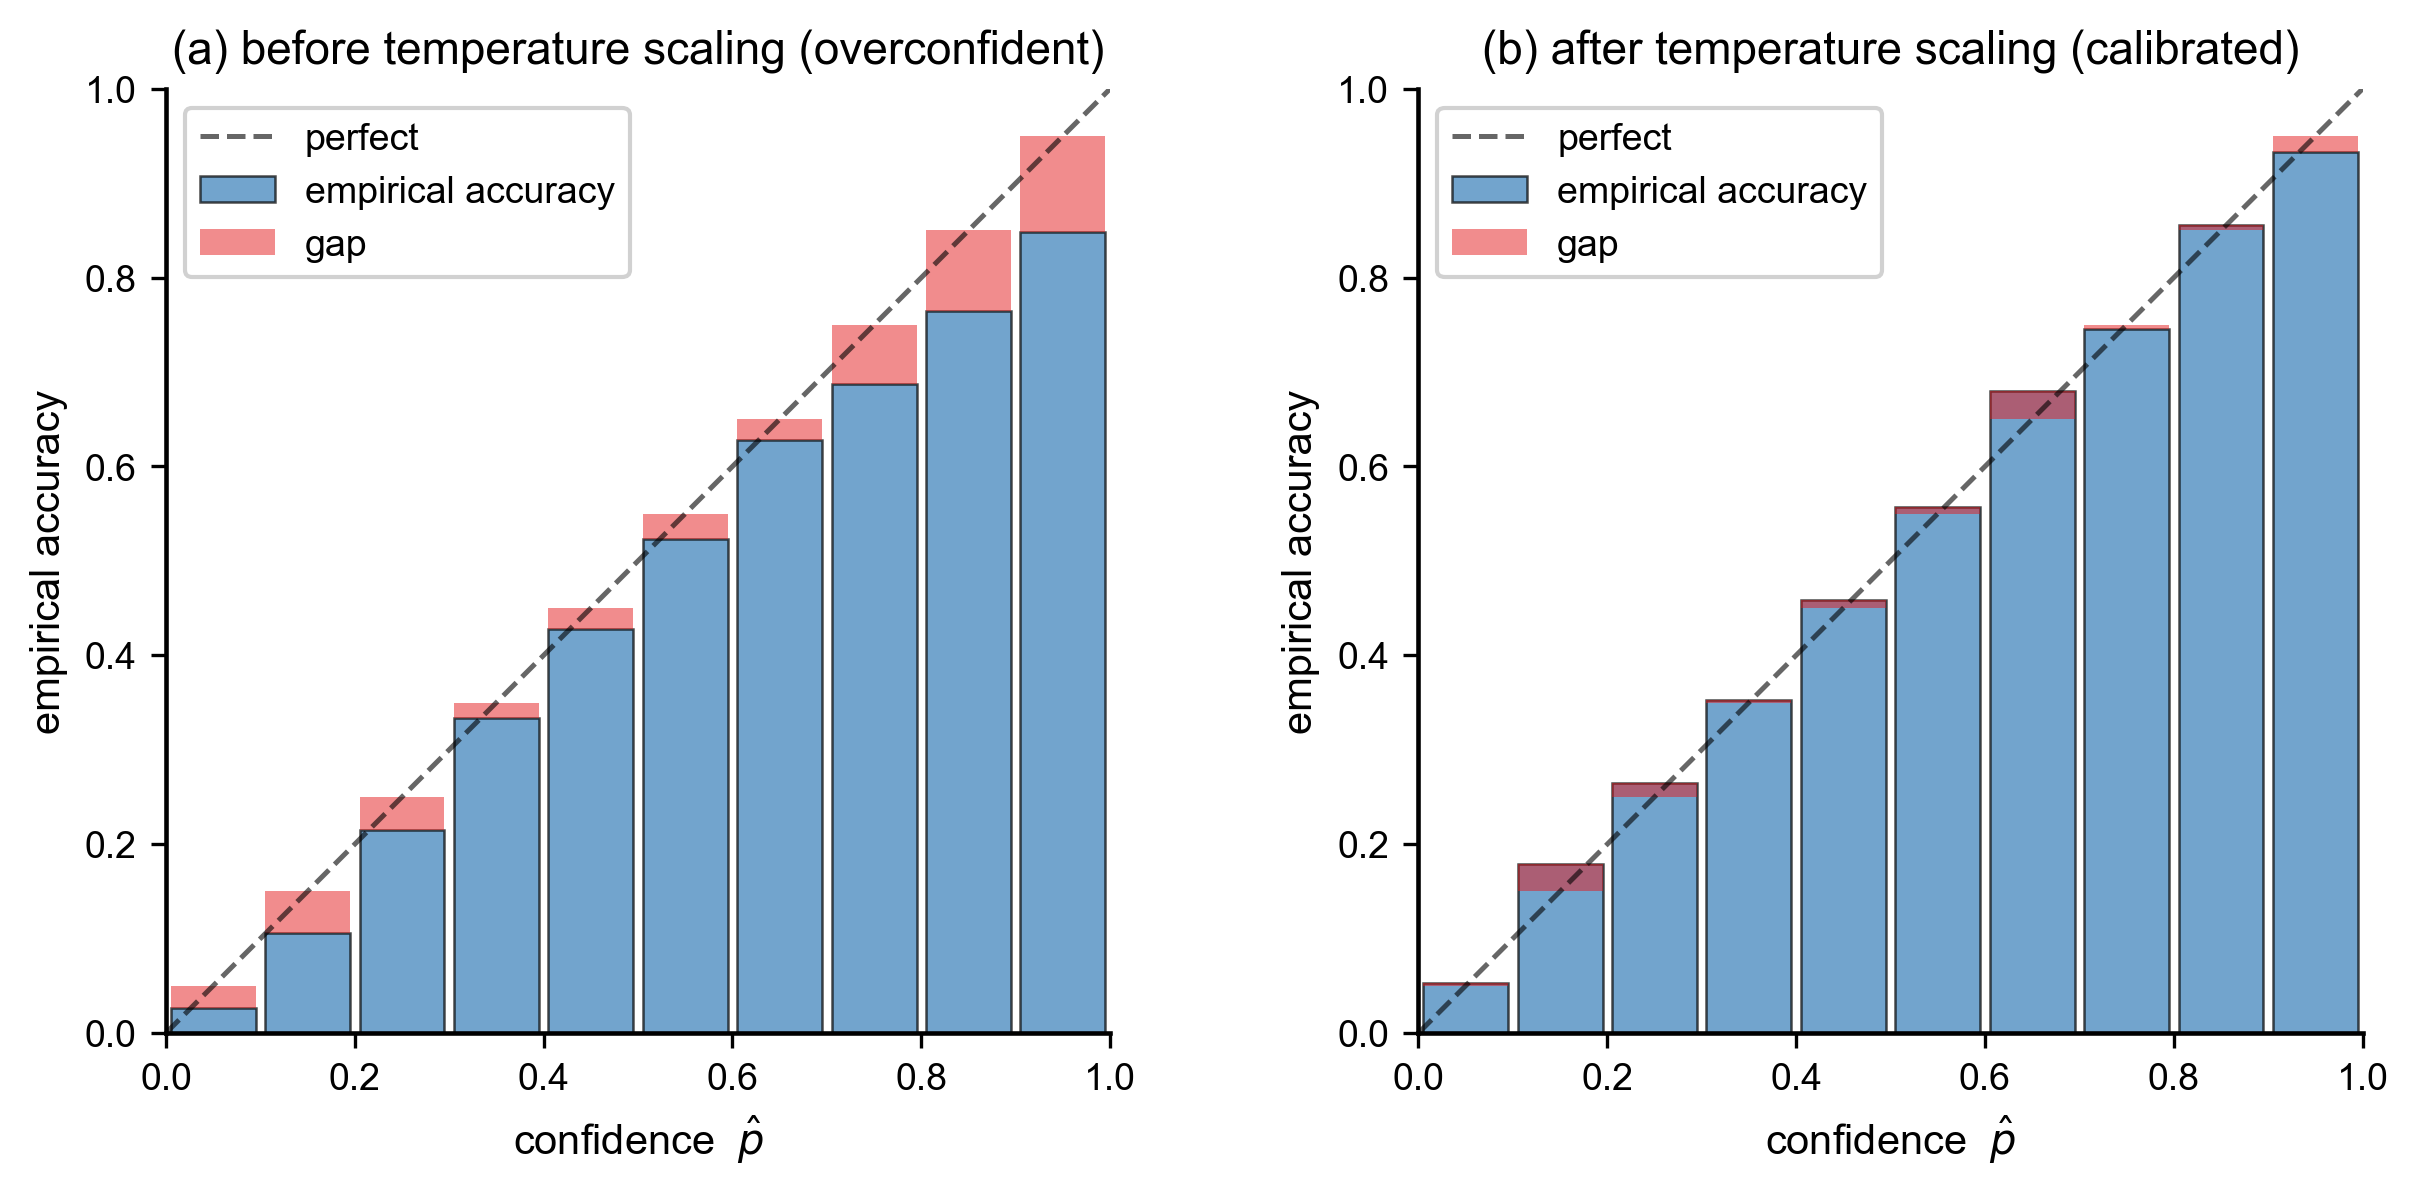
\includegraphics[width=0.92\textwidth]{ch2_reliability_diagram.png}
    \caption{\textbf{[概念示意图]} 温度缩放前后的可靠图对比。左图为校准前，预测置信度系统性高于经验准确率（红色为 gap）；右图为拟合 $T^{\ast}$ 后，经验准确率贴近对角线，过度自信被有效修正。本图用合成数据演示温度缩放的作用机制，不是本文实验产生的可靠图。}
    \label{fig:ch2-reliability}
\end{figure}

\section{召回约束门控与阈值选择}

\subsection{工作点指标}
给定工作阈值 $\tau \in [0, 1]$，判决规则 $\hat{y}(x) = \mathbb{1}[p_{\rm cal}(x) \geq \tau]$。设评估集 $\mathcal{D}_{\rm eval}$ 中正常样本（$y=0$）集合为 $\mathcal{N}$、异常样本（$y=1$）集合为 $\mathcal{A}$，基本工作点指标定义为
\begin{align}
\mathrm{Recall}(\tau) &= \frac{1}{|\mathcal{A}|}\sum_{x \in \mathcal{A}} \mathbb{1}[p_{\rm cal}(x) \geq \tau], \label{eq:recall}\\
\mathrm{Spec}(\tau) &= \frac{1}{|\mathcal{N}|}\sum_{x \in \mathcal{N}} \mathbb{1}[p_{\rm cal}(x) < \tau], \label{eq:spec}\\
\mathrm{Prec}(\tau) &= \frac{\sum_{x \in \mathcal{A}}\mathbb{1}[p_{\rm cal}(x) \geq \tau]}{\sum_{x \in \mathcal{N} \cup \mathcal{A}}\mathbb{1}[p_{\rm cal}(x) \geq \tau]}. \label{eq:prec}
\end{align}
式~\eqref{eq:recall} 至 \eqref{eq:spec} 为条件概率估计，不依赖于先验 $\mathbb{P}[y=1]$，因此在训练集与部署场景先验不一致时仍保持可比性。式~\eqref{eq:prec} 的分母依赖于联合分布，对先验敏感。

\subsection{Elkan 成本敏感阈值}
给定真实后验概率 $\eta(x) = \mathbb{P}[y = 1 \mid x]$ 与错分代价矩阵 $\mathbf{C}$，其中 $c_{\rm FP} = C_{1,0}$ 为假阳性代价（将正常误判为异常的成本，对应多出的人工复核量）、$c_{\rm FN} = C_{0,1}$ 为假阴性代价（将异常漏判为正常的成本，对应漏检缺陷的工程风险），且真阳性、真阴性代价均为零。Elkan\cite{elkan2001foundations} 在 IJCAI 2001 上证明，最小化期望代价的贝叶斯最优决策规则为 $\hat{y}(x) = \mathbb{1}[\eta(x) \geq \tau^{\ast}]$，其中
\begin{equation}
\tau^{\ast} = \frac{c_{\rm FP}}{c_{\rm FP} + c_{\rm FN}}.
\label{eq:elkan-threshold}
\end{equation}
即在校准概率空间下，最优阈值仅由两类错分代价的相对比决定，与先验分布 $\mathbb{P}[y]$ 无关。该结果的前提条件是 $\eta(x)$ 已被校准——若分类器输出的 $\hat{\eta}(x)$ 存在系统性偏差，直接将式~\eqref{eq:elkan-threshold} 的数值代入会产生次优决策；反之，若在独立校准集上完成了温度缩放等事后校准，$p_{\rm cal}(x)$ 即可视为 $\eta(x)$ 的良好估计，式~\eqref{eq:elkan-threshold} 才具有直接可用性。这一逻辑链明确了\textbf{概率校准是成本敏感决策的前提}，也是本文将 2.2 与 2.3 两节紧接安排的理论依据。

式~\eqref{eq:elkan-threshold} 对本文研究的第二个直接推论是\textbf{阈值与训练解耦}：部署场景下若应用先验或错分代价发生变化，只需在目标场景的校准集上重新搜索 $\tau^{\ast}$，网络参数 $\theta$ 无需重训。这一解耦性允许本文在单一训练集上训练一次模型，然后在不同召回下界（99.5\% 与 99.0\%）或不同部署先验下分别报告工作点指标，避免陷入"每换一个场景重训一次"的组合爆炸。

\subsection{召回约束下的阈值搜索}
在排水管道高召回门控场景下，错分代价难以显式定价：漏检一处严重缺陷（$c_{\rm FN}$）的实际后果取决于管道等级、水文条件与下游居民分布，而非一个可预先约定的标量值。相反，工程实践中通常以\textbf{固定召回下界}作为安全边界——例如要求模型在验证集上保证 99.5\% 的异常召回率，其余 specificity 越高越好。这种"约束优化"视角避免了错分代价的主观定价问题，同时保留了成本敏感分类的理论根基：由式~\eqref{eq:elkan-threshold} 可知，任意满足召回约束的工作点都对应某组隐式代价比例。

形式化地，给定召回下界 $R_0 \in (0, 1)$，召回约束最优阈值定义为
\begin{equation}
\tau_{R_0} = \min\bigl\{\tau \in [0, 1] : \mathrm{Recall}(\tau) \geq R_0\bigr\},
\label{eq:constrained-threshold}
\end{equation}
即满足召回约束的最小阈值。由于 Recall 是 $\tau$ 的\textbf{非增阶梯函数}（每当 $\tau$ 越过一个异常样本的校准分数时下降 $1/|\mathcal{A}|$），式~\eqref{eq:constrained-threshold} 的最优解就是使召回率恰好跨越 $R_0$ 的那个断点。实际计算方法为：在 val-op 集上计算所有异常样本的 $p_{\rm cal}$ 值并降序排序，取第 $\lceil R_0 \cdot |\mathcal{A}| \rceil$ 大的分数作为 $\tau_{R_0}$。该过程时间复杂度为 $O(|\mathcal{A}|\log|\mathcal{A}|)$，在万量级评估集上毫秒级完成，可对每个训练检查点逐 epoch 执行。

在该阈值下，正常样本拦截率的条件分布表达式为
\begin{equation}
\mathrm{Spec@R}_0 = \mathrm{Spec}(\tau_{R_0}) = F_0(\tau_{R_0}),
\label{eq:spec-at-recall}
\end{equation}
其中 $F_0(\tau) = \mathbb{P}[p_{\rm cal}(x) < \tau \mid y = 0]$ 为正常类的校准概率累积分布函数。式~\eqref{eq:spec-at-recall} 揭示了一项对跨场景部署至关重要的性质——\textbf{Spec@R$_0$ 是条件分布 $F_0$ 上的点值，与类别先验 $\mathbb{P}[y]$ 无关}。也就是说，即使部署场景下正常帧与异常帧的比例大幅偏离训练集（例如实际巡检中正常帧可能占 95\% 以上，而训练集中为工程设计取 50\%），Spec@R$_0$ 在同一模型上的取值仍然稳定——变化的只是 $\tau_{R_0}$ 的具体数值，不是模型本身的判别能力。这一先验无关性让本文可以在一套训练集上训练、在任意先验场景下重搜索阈值而数字可比，支撑了第~5 章对不同召回下界（99.5\% 与 99.0\%）的并列报告。

图~\ref{fig:ch2-threshold} 以两类样本的分数分布直观呈现了该阈值搜索过程：$\tau_{R_0}$ 左侧的正常样本贡献 Spec@R$_0$（真阴性），右侧的异常样本满足召回约束（真阳性）。与将召回约束融入训练损失的方案\cite{kumar2021constrained} 相比，本文采用的事后阈值搜索具有两项工程优势：一是不改变训练流程，与 YOLO 等开源框架无缝兼容；二是允许对同一训练好的模型在多个召回下界上分别报告结果，避免"一个召回对应一次训练"的成本。

\begin{figure}[H]
    \centering
    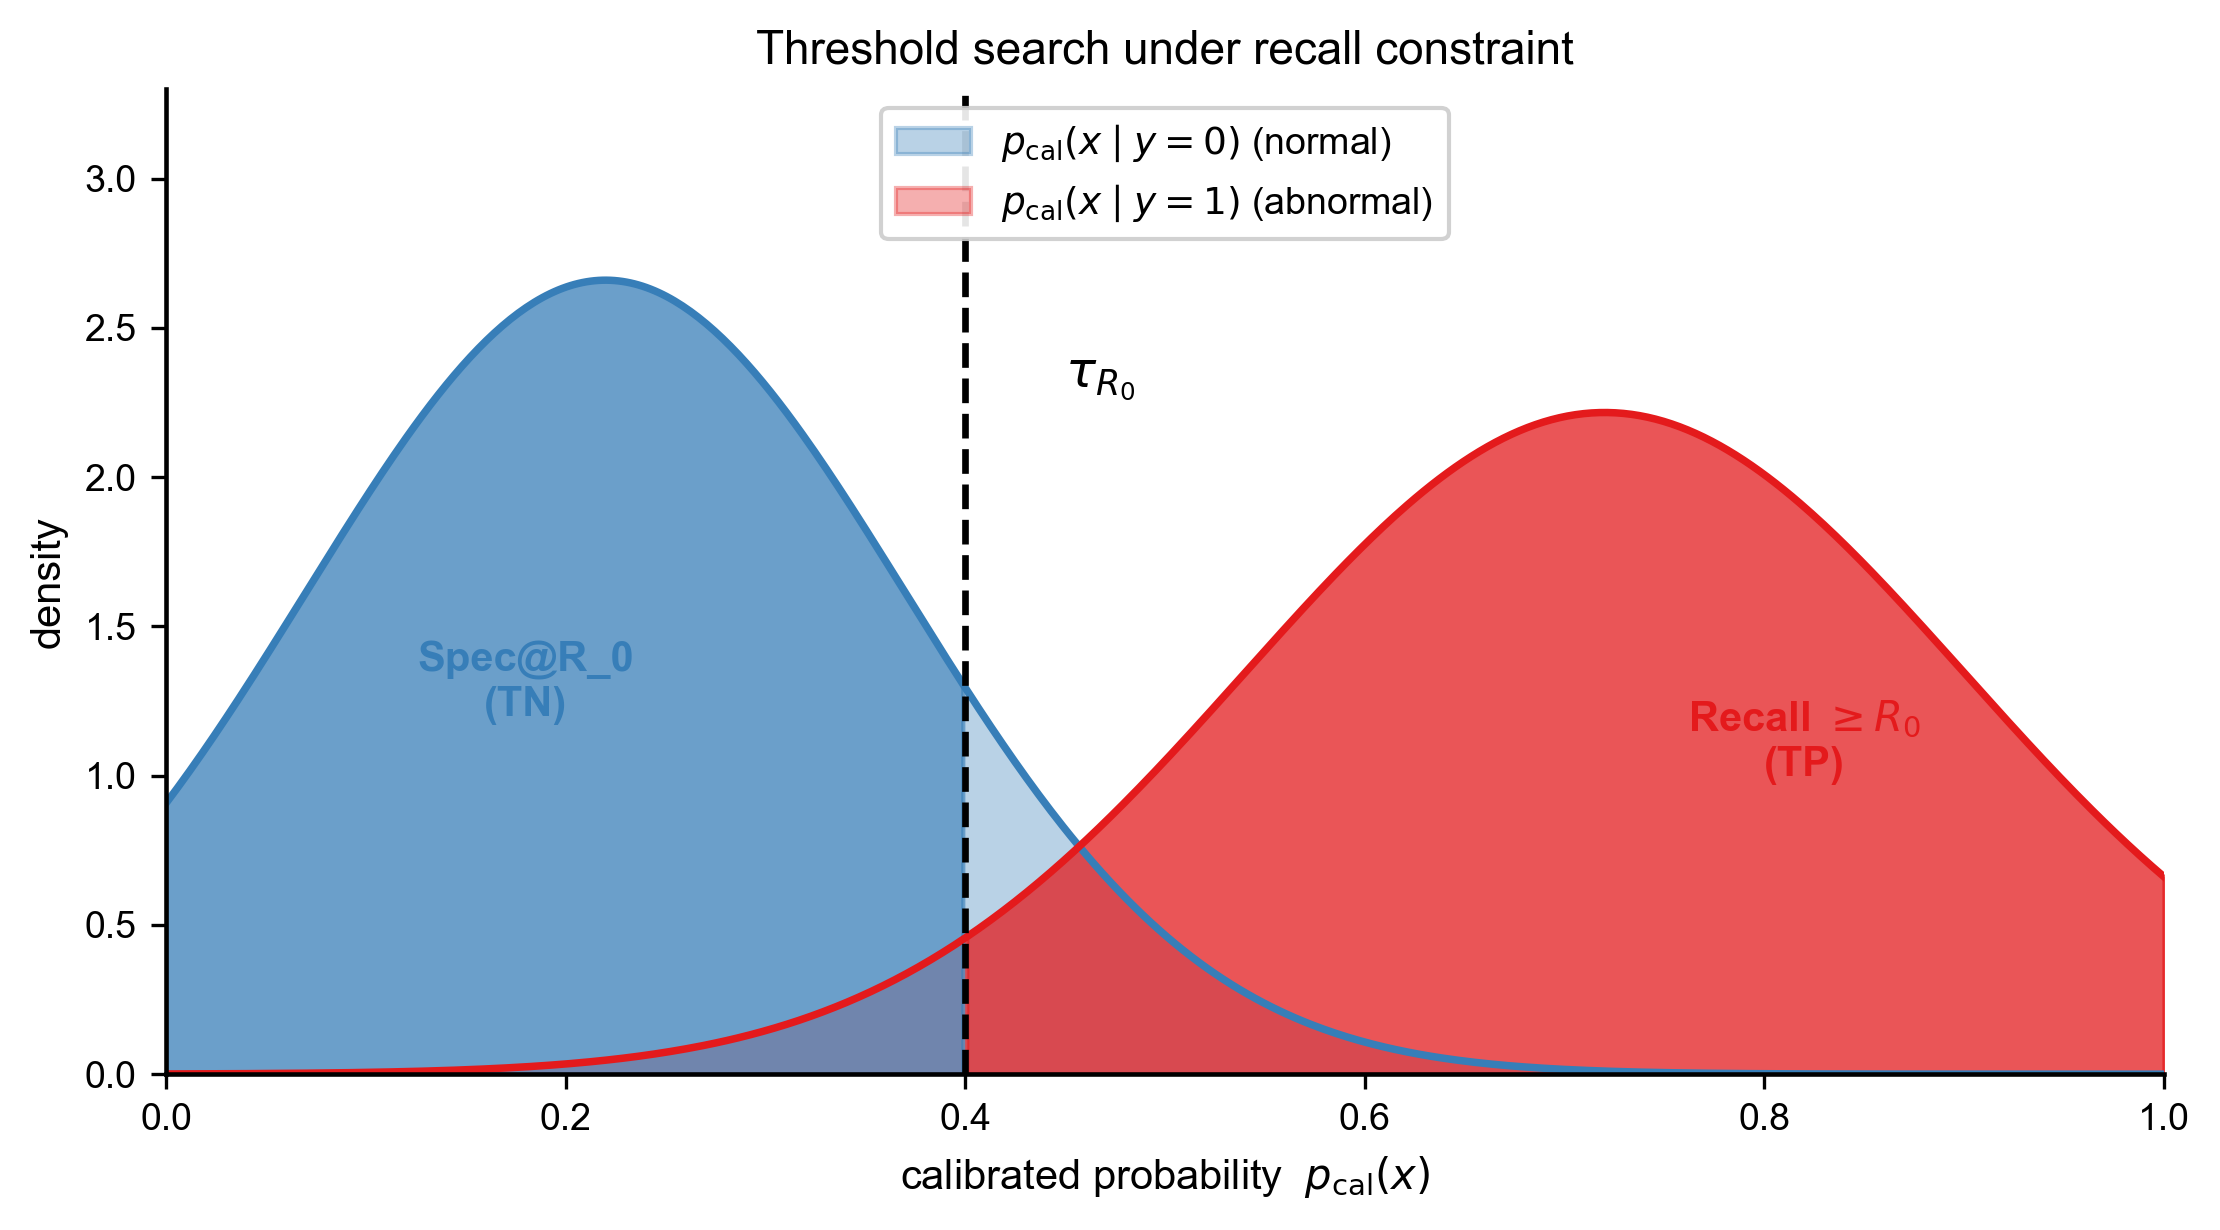
\includegraphics[width=0.82\textwidth]{ch2_threshold_search.png}
    \caption{\textbf{[概念示意图]} 召回约束下的阈值搜索。蓝色与红色分别为正常类与异常类在校准概率空间上的分布；黑色虚线为满足召回约束 $R_0$ 的最小阈值 $\tau_{R_0}$。本图用两个示意高斯分布演示阈值搜索的几何含义，不是本文实验产生的真实分数分布。}
    \label{fig:ch2-threshold}
\end{figure}

\subsection{四元字典序排序规则}
当多个模型在 $\mathrm{Spec@R}_0$ 上取值相同（小样本评估下尤其常见，因为 specificity 的最小步长为 $1/|\mathcal{N}|$），需要辅助指标打破平局。本文采用四元字典序（lexicographic order）排序规则：
\begin{equation}
\mathrm{rank}(\theta) = \mathrm{lex}\bigl(\mathrm{Spec@R99.5}, \mathrm{Spec@R99.0}, \mathrm{Prec@R99.0}, -\mathrm{PTR@R99.0}\bigr),
\label{eq:lex-rank}
\end{equation}
其中 PTR（pass-through rate，通过率）定义为 $\mathrm{PTR}(\tau) = \frac{1}{|\mathcal{D}_{\rm eval}|}\sum_{x \in \mathcal{D}_{\rm eval}}\mathbb{1}[p_{\rm cal}(x) \geq \tau]$，即进入下一阶段的样本占比，前三项越大越优，最后一项越小越优（更低的通过率意味着更少的人工复核量）。

\section{样本价值评估的四信号框架}

本文采用四个正交信号刻画候选样本的训练价值：边界风险 $R$、邻域密度 $D$、训练动态 $T$、扰动一致性 $C$。四信号的概念对比见图~\ref{fig:ch2-rdtc}，各自形式化定义如下。

\subsection{边界风险信号 $R$}
边界风险刻画样本在当前模型判别面附近的不确定性，其思想可追溯至 Lewis 与 Gale\cite{lewis1994sequential} 提出的不确定性采样：在主动学习框架下，距离决策边界最近的样本被认为携带最多的"新信息"——模型对这些样本的判断最犹豫，学到它们可以最有效地修正决策面。Settles\cite{settles2009active} 的综述将这一思想系统化为三种变体（least-confidence、margin、entropy），三者在二分类场景下数学等价。

本文选择在\textbf{校准概率空间}定义边界风险，而非直接使用原始 logit。校准后的 $p_{\rm cal}(x)$ 对应"模型估计的类别后验概率"，决策边界恰为 $p = 0.5$；样本到边界的距离 $|p_{\rm cal}(x) - 0.5|$ 直接等于 $|\eta(x) - 0.5|$ 的估计，具有清晰的概率语义。定义
\begin{equation}
R(x) = \frac{1}{\bigl|\,p_{\rm cal}(x) - 0.5\,\bigr| + \epsilon},
\label{eq:signal-R}
\end{equation}
其中 $\epsilon > 0$ 为数值稳定项（本文取 $\epsilon = 10^{-6}$）。$R(x)$ 越大表示样本越靠近决策边界，对应模型判别越犹豫。

$R$ 信号与 Goldilocks 假设的联系在于：Lewis 与 Gale\cite{lewis1994sequential} 原始的"uncertainty sampling"暗含的是\textbf{边界距离与价值单调递增}的线性假设（越难越有价值）；而 Swayamdipta 等\cite{swayamdipta2020cartography} 的 Dataset Cartography 观察到——在深度网络训练场景下——真正价值最大的样本并非最靠近边界的那一批，而是"近边界但非边界"的中间层。因此，$R$ 信号在本文中同时承担两个任务：作为候选样本的可计算排序依据（这一任务与 Lewis 1994 一致），以及作为验证 Goldilocks 假设的正交信号之一（这一任务需要进一步检验非单调价值响应是否成立）。第~6 章将通过按 $R$ 分位数分层的消融实验回答后一个问题。

\subsection{邻域密度信号 $D$}
邻域密度刻画样本在特征空间中的局部稠密程度，其动机源自 Sener 与 Savarese\cite{sener2018active} 的核心集选样框架。他们证明，在主动学习的泛化误差上界中，选样策略的关键作用是最小化未标注集到已标注集的\textbf{几何覆盖半径}——即所选子集应在特征空间中作为未标注集的"代表点集"（core set）。这一几何视角补充了边界风险 $R$ 的纯信号视角：$R$ 只看单个样本与边界的距离，$D$ 则看样本在流形结构中的邻域分布。

设 $\phi : \mathcal{X} \to \mathbb{R}^d$ 为 YOLO11-cls 倒数第二层（全局池化后）的特征提取映射，$\mathrm{kNN}(x)$ 为 $x$ 在特征空间中按余弦相似度计算的 $k$ 近邻集合，邻域密度定义为
\begin{equation}
D(x) = \frac{1}{k}\sum_{y \in \mathrm{kNN}(x)} \frac{\phi(x)^{\top}\phi(y)}{\|\phi(x)\|\,\|\phi(y)\|}.
\label{eq:signal-D}
\end{equation}
$D(x)$ 越大表示样本位于特征空间的稠密聚类区域（有大量相似邻居）；$D(x)$ 越小表示样本位于稀疏区域或流形边缘（近邻稀少且不相似）。

$D$ 信号与 $R$ 信号的\textbf{正交性}可从信息内容上论证：$R$ 仅依赖单个样本的模型输出 $p_{\rm cal}(x)$，不涉及任何其他样本；$D$ 依赖样本之间的特征相似度结构，不涉及模型判别面。两者在极端情形下可以完全不一致——位于特征空间稠密聚类中心的样本（高 $D$）可能离决策边界很远（低 $R$）；位于边界附近的孤立样本（高 $R$）可能在特征空间中是稀疏点（低 $D$）。本文的核心假设之一正是利用这种正交性：\textbf{若 Goldilocks 效应在 $R$ 和 $D$ 两个独立测量方向上同时复现，则该效应不是单一测量方法的系统偏差，而是候选池样本价值分布的结构性规律}。这一假设将在第~6 章通过 $D$ 信号的独立分位数扫描实验验证。

$D$ 信号对应 Goldilocks 假设的物理解释也与 $R$ 不同：最稠密区域的样本（$D$ 最大）意味着模型已见过大量相似样本，继续添加此类样本的边际价值低；最稀疏区域的样本（$D$ 最小）则可能是采集噪声、视角异常或分布外异常点，训练价值低但训练成本高；中间密度的样本代表"有足够上下文、但尚未被充分覆盖的子流形"，这与 Goldilocks 假设所预测的"中间层最有价值"一致。

\subsection{训练动态信号 $T$}
训练动态将时间维度引入样本价值刻画。Toneva 等\cite{toneva2019empirical} 在 ICLR 2019 上首次提出"遗忘事件"（forgetting events）概念：统计每个样本在训练过程中被"学会"后又被"遗忘"的次数，发现高遗忘次数的样本大多是标注错误或真正困难的边界样本。Swayamdipta 等\cite{swayamdipta2020cartography} 在 EMNLP 2020 上将该思路细化为\textbf{数据集制图}（dataset cartography）：对每个样本跟踪其跨 epoch 的预测置信度轨迹，用置信度均值与标准差两个坐标将样本映射到二维空间，识别出"易学"、"模糊"与"难学"三个区域，并发现模糊区域（置信度均值中等、标准差较大）的样本对模型泛化贡献最大。这一发现正是本文 Goldilocks 假设的直接思想来源。

设 $p_{{\rm cal},t}(x)$ 为第 $t$ 个训练轮次后、经温度缩放校准的异常概率；选取一组采样时间点 $\mathcal{T} = \{t_1, t_2, \ldots, t_L\}$（本文取训练中后期的若干 epoch，以覆盖模型基本收敛后的稳定波动），训练动态信号定义为
\begin{equation}
T(x) = \sqrt{\frac{1}{L}\sum_{t \in \mathcal{T}}\bigl(p_{{\rm cal},t}(x) - \bar{p}(x)\bigr)^2}, \quad \bar{p}(x) = \frac{1}{L}\sum_{t \in \mathcal{T}} p_{{\rm cal},t}(x).
\label{eq:signal-T}
\end{equation}
$T(x)$ 即样本校准概率在采样点上的标准差。$T(x)$ 越大表示样本在训练过程中预测越不稳定（模型对其态度反复摇摆），对应 Swayamdipta 等\cite{swayamdipta2020cartography} 所识别的"模糊"样本；$T(x)$ 越小表示样本在训练过程中被稳定分类（要么一直被判为正常，要么一直被判为异常）。

$T$ 信号与 $R$、$D$ 的\textbf{正交性}体现在\textbf{测量维度}上：$R$ 是\textbf{单样本、单 checkpoint 的空间测量}（样本到边界的静态距离），$D$ 是\textbf{多样本、单 checkpoint 的空间测量}（样本在特征空间的邻域结构），$T$ 则是\textbf{单样本、多 checkpoint 的时间测量}（样本在训练轨迹上的动态波动）。三者分别对应"空间静态"、"空间结构"与"时间动态"三个独立视角，构成对样本价值的三重近似正交测度。若三个测度在 Goldilocks 效应上给出一致的非单调响应，则该效应超越了任一单一测量范式，具有跨方法论层面的稳健性。这一跨信号一致性检验是第~6 章的核心实验设计。

\subsection{扰动一致性信号 $C$}
扰动一致性引入空间扰动作为第四维测度。Gal 等\cite{gal2017deep} 在 ICML 2017 上提出深度贝叶斯主动学习框架：通过对模型施加蒙特卡洛 Dropout，对同一输入产生多次预测，预测方差即为 Bayesian 近似下的样本不确定性。Beluch 等\cite{beluch2018power} 进一步证明，用模型集成替代 Dropout 可产生更可靠的不确定性估计。两者的共同内核为\textbf{扰动下预测稳定性}：若模型对同一样本的预测在扰动下剧烈变化，则该样本位于模型判别面附近或处于模型学习能力的边缘，具有较高的信息量。

本文将扰动源从模型侧（Dropout、Ensemble）迁移到\textbf{输入侧}——测试时增强（test-time augmentation, TTA）。设 $\mathcal{A}$ 为一组保持语义的输入扰动（如水平翻转、随机裁剪、轻度色彩抖动、轻度模糊等，每种扰动不改变样本的类别标签），每次从 $\mathcal{A}$ 中采样一种扰动 $a$ 并得到视图 $a(x)$，扰动一致性信号定义为
\begin{equation}
C(x) = 1 - \mathrm{Var}_{a \sim \mathcal{A}}\bigl[\,p_{\rm cal}(a(x))\,\bigr].
\label{eq:signal-C}
\end{equation}
$C(x)$ 越大表示样本在扰动下预测稳定（模型的判断"经得起扰动"），越小表示样本预测不稳（轻微扰动即可改变判断）。

将扰动源放在\textbf{输入侧而非模型侧}的理由有三：其一，TTA 不需要在推理时做多次前向传播于不同模型副本，工程成本低；其二，TTA 直接模拟部署场景下输入自然变化（光照、角度、轻度模糊）对模型判断的鲁棒性，语义上更贴近"高价值样本应当在真实扰动下仍判对"的工程诉求；其三，TTA 与 YOLO11-cls 本身的训练增强完全解耦——训练用的增强策略即便固定，推理时的 TTA 仍可作为独立测量工具。

$C$ 信号与 $R$、$D$、$T$ 构成\textbf{四维正交测量系统}的最后一维：$R$ 为单样本空间静态、$D$ 为多样本空间结构、$T$ 为单样本时间动态、$C$ 为单样本扰动响应。四者的数学计算彼此独立，物理含义不相互蕴含——模型对某样本在原始输入上接近 $p = 0.5$（$R$ 高）并不必然意味着其预测在扰动下不稳（$C$ 低），反之亦然。四信号的正交性使其能够独立地检验 Goldilocks 效应——若四个信号的分位数消融都显示中间层样本价值高于极端样本，则该效应具有最强的跨方法一致性。

\begin{figure}[H]
    \centering
    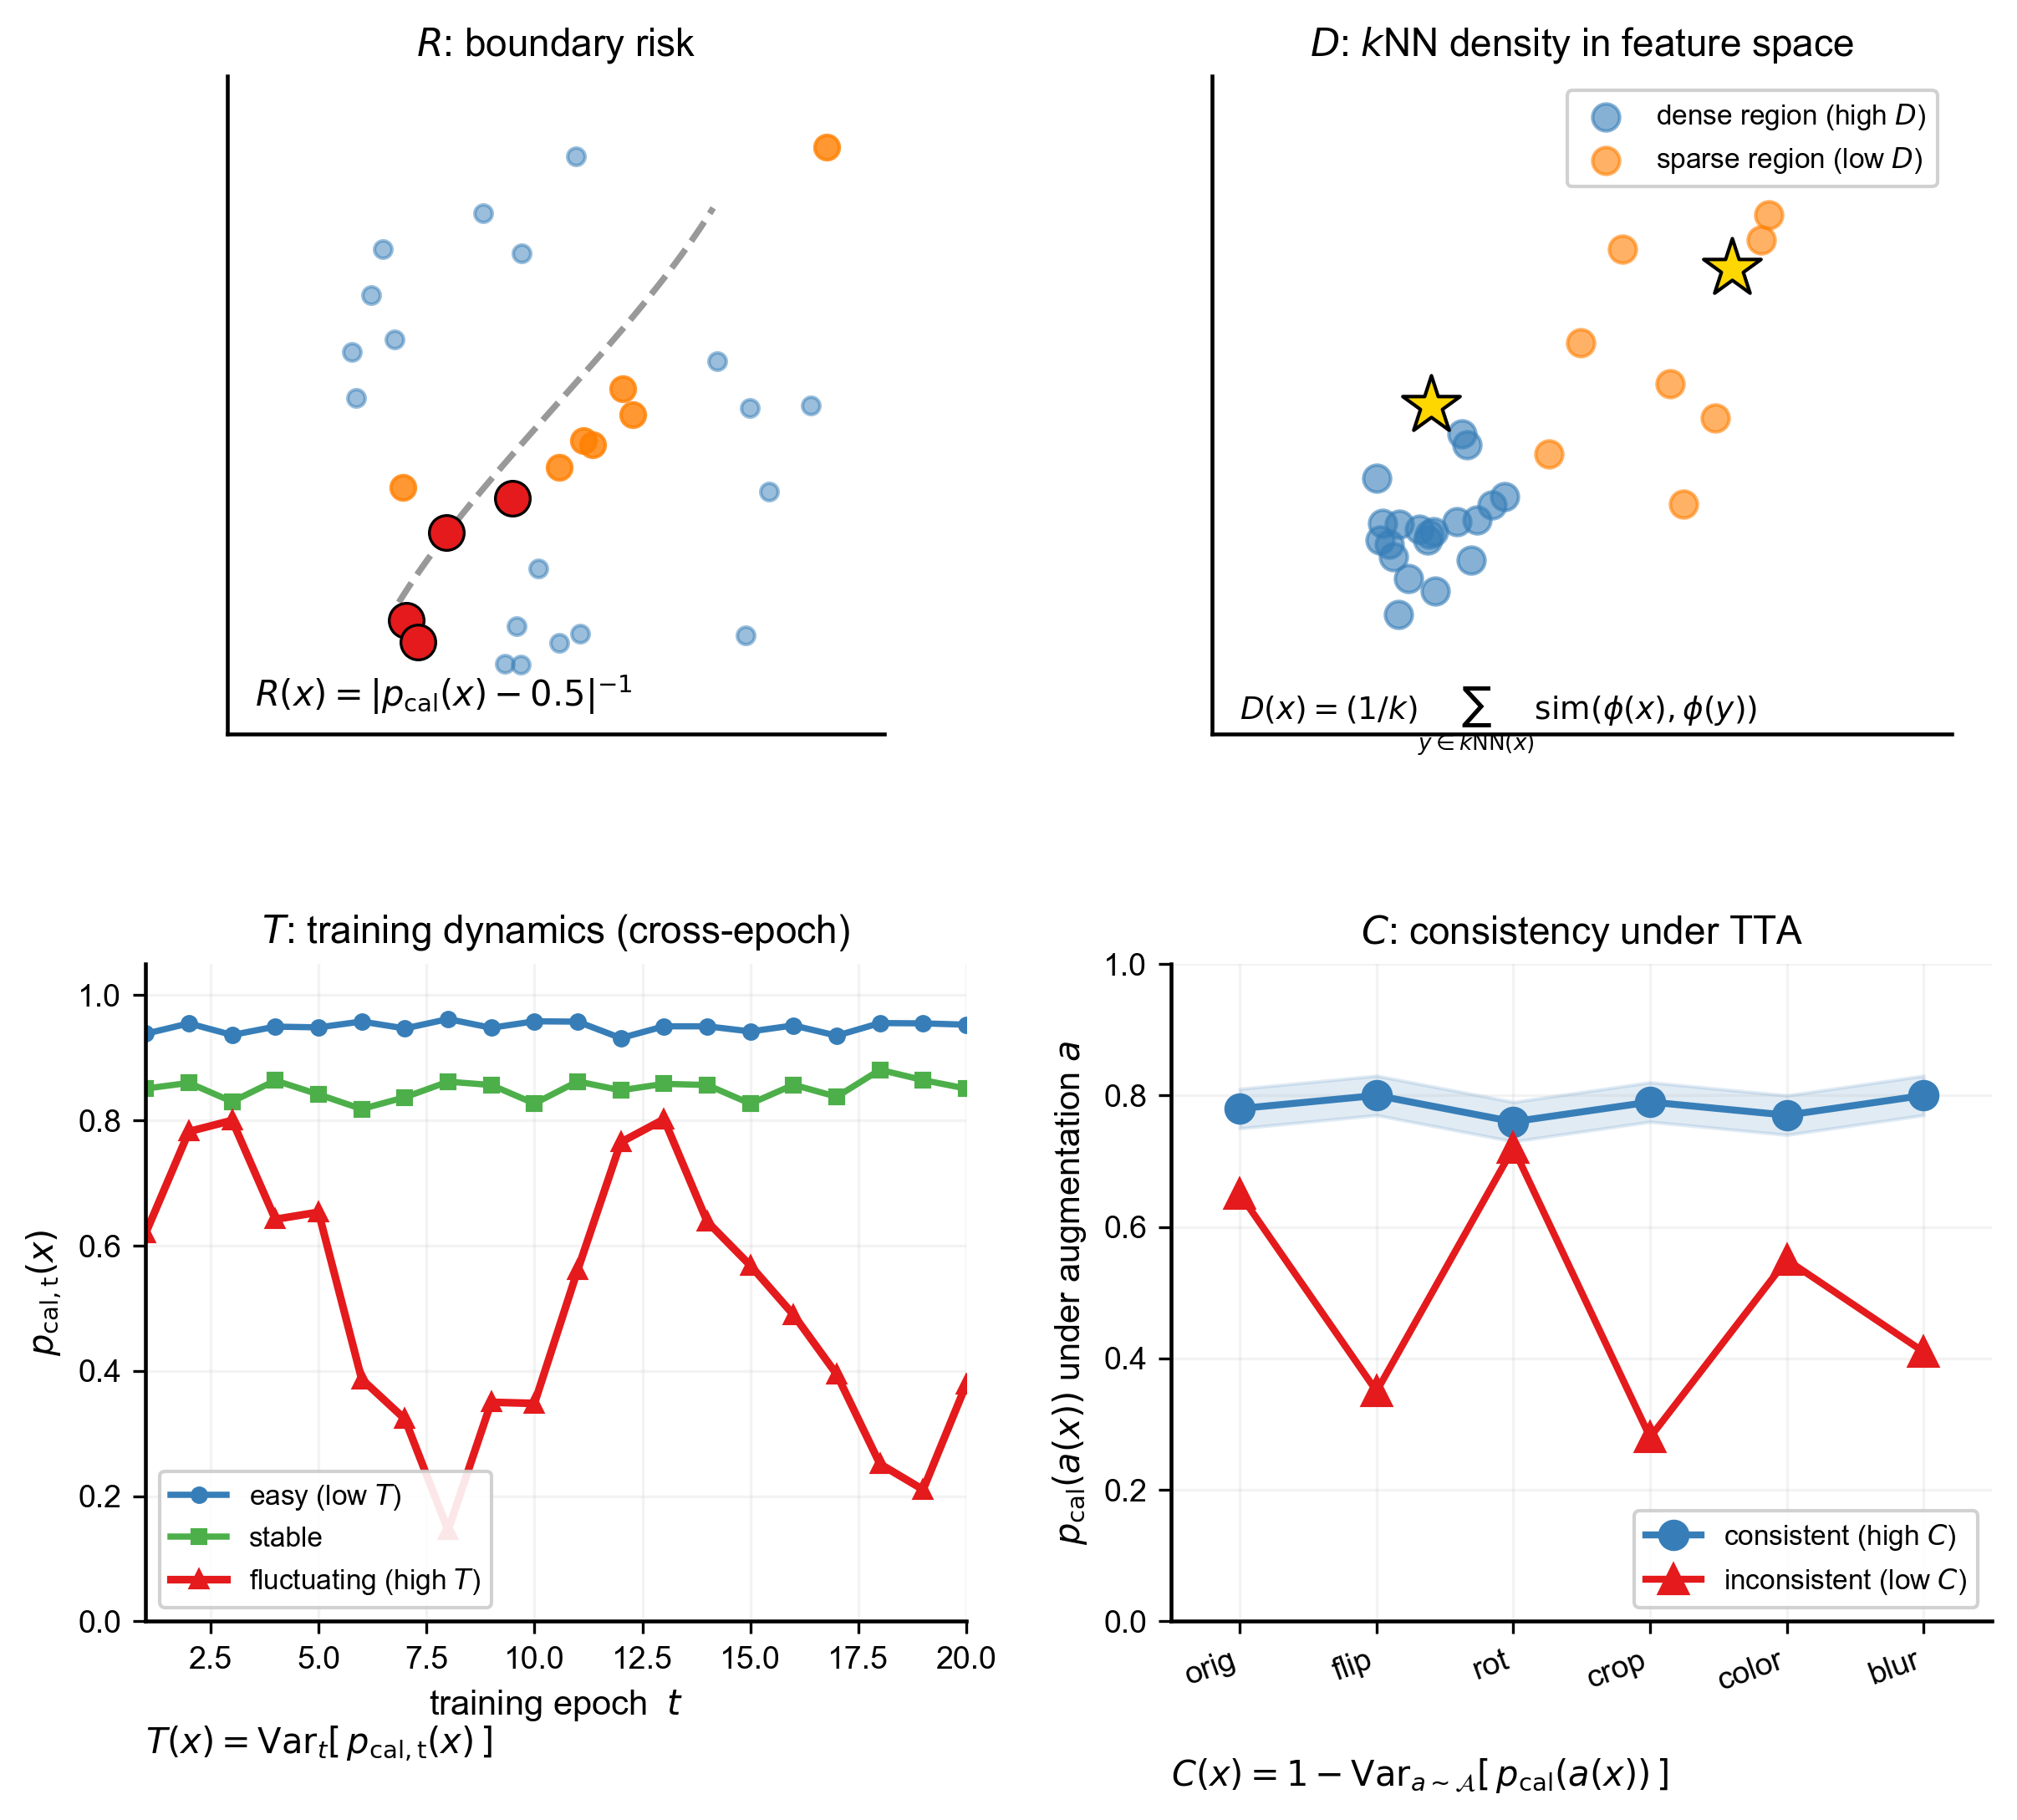
\includegraphics[width=\textwidth]{ch2_rdtc_four_signals.png}
    \caption{\textbf{[概念示意图]} RDTC 四信号概念示意。$R$（左上）衡量样本到决策边界的距离；$D$（右上）衡量特征空间邻域密度；$T$（左下）衡量跨 epoch 预测波动；$C$（右下）衡量输入扰动下的预测稳定性。四信号分别捕捉静态、空间、时间、扰动四个正交维度。本图各子面板用合成样本与模拟轨迹演示信号的直觉，不是本文实验产生的真实信号值。}
    \label{fig:ch2-rdtc}
\end{figure}

\subsection{Goldilocks 非单调价值假设}
Swayamdipta 等\cite{swayamdipta2020cartography} 在 EMNLP 2020 上提出，最有训练价值的样本并非信号极值位置，而是中间层的模糊样本——最难样本中混入的标注噪声与分布外异常反而损害训练效果。这一假设与本文所验证的跨信号 Goldilocks 效应一致。图~\ref{fig:ch2-goldilocks} 给出其概念化示意。

\begin{figure}[H]
    \centering
    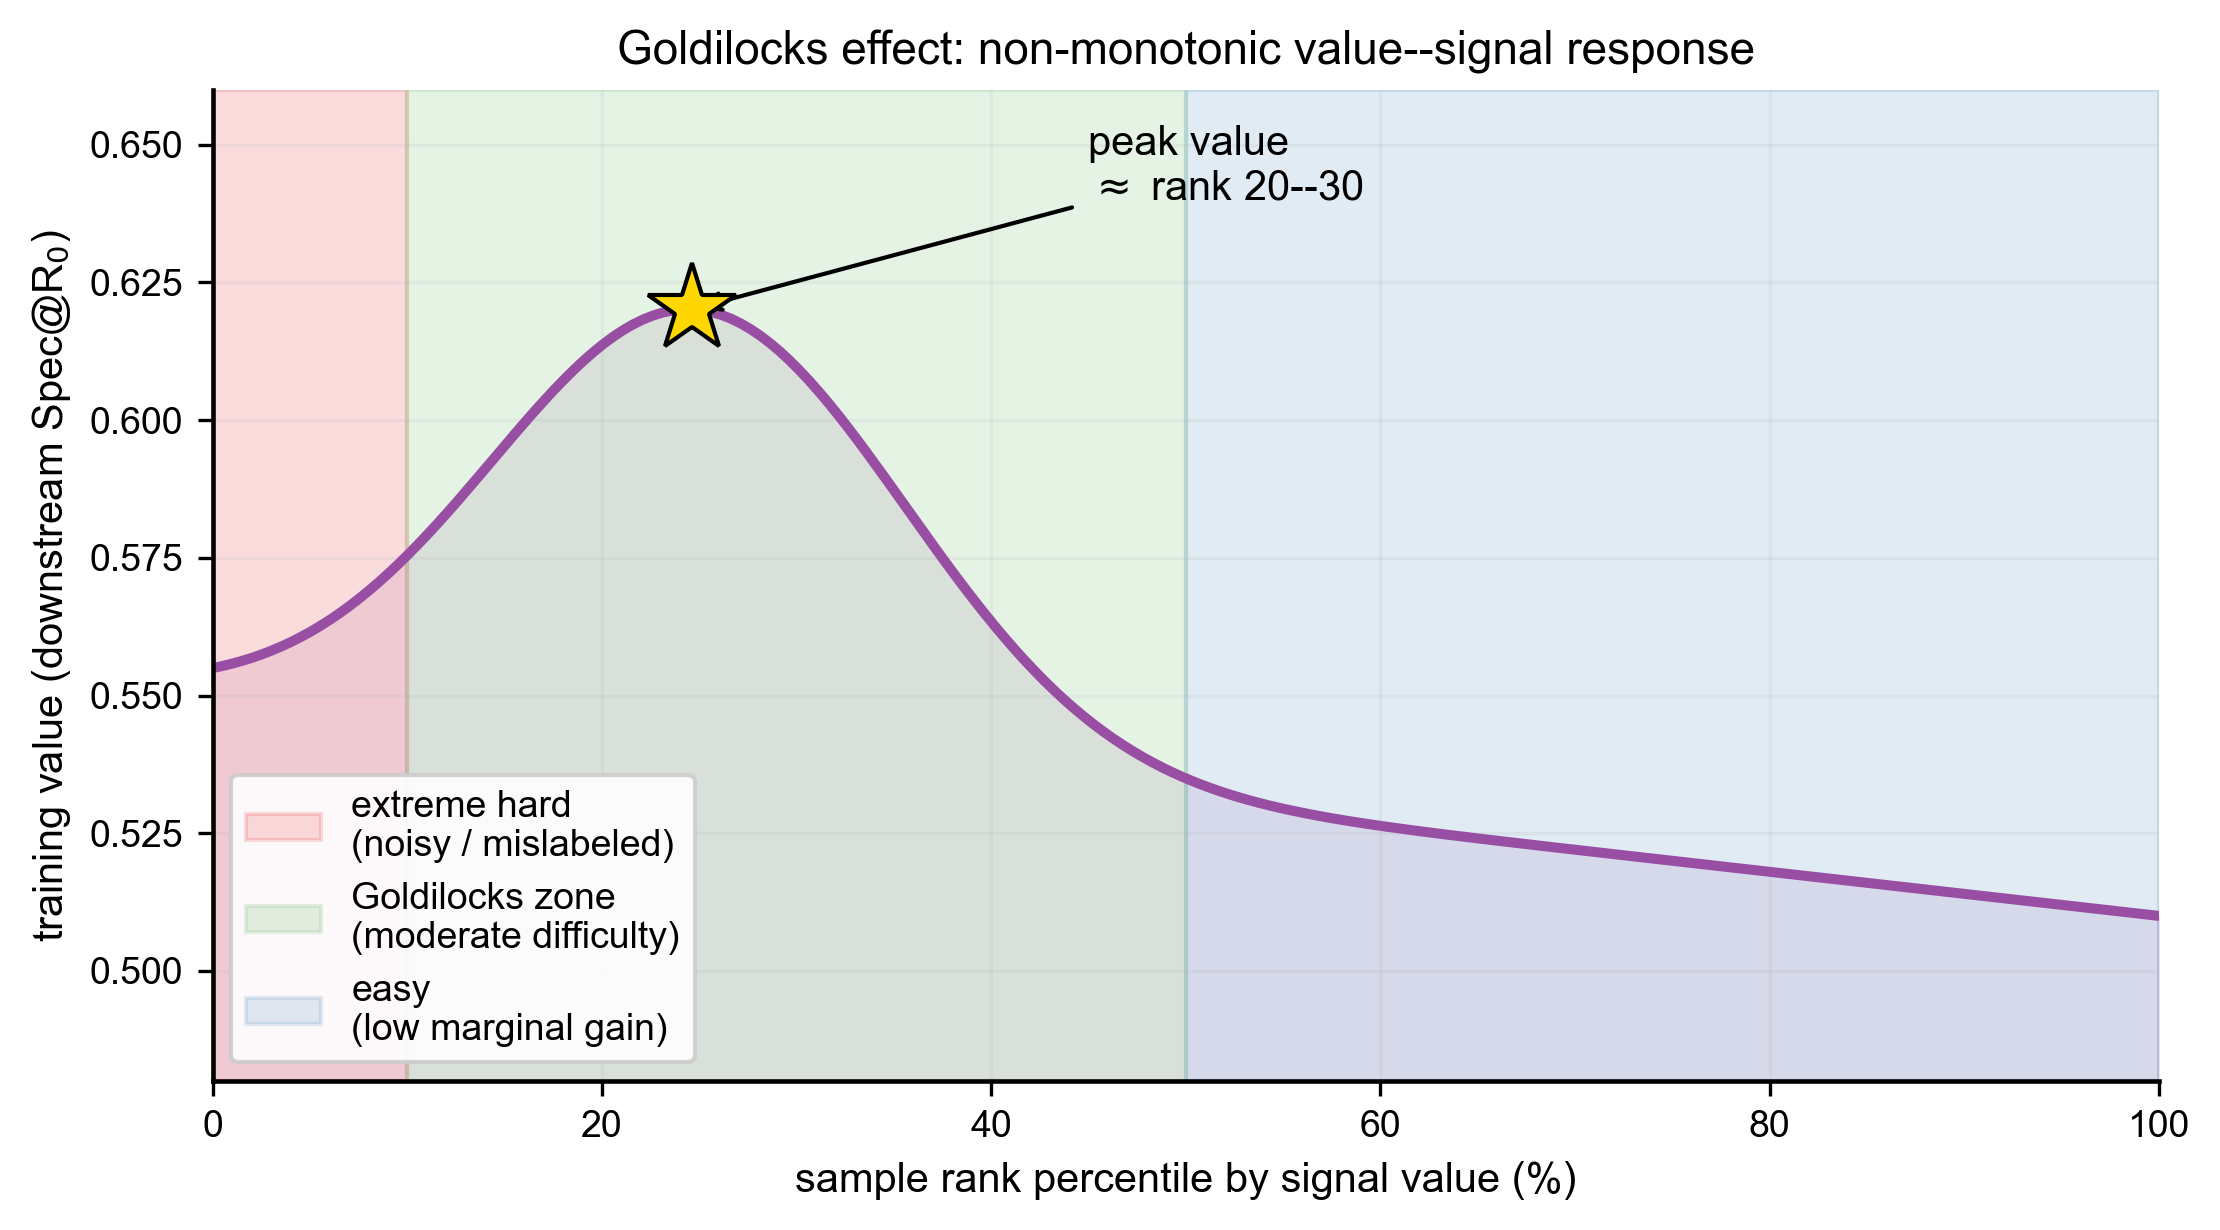
\includegraphics[width=0.82\textwidth]{ch2_goldilocks_curve.png}
    \caption{\textbf{[概念示意图]} Goldilocks 效应的概念示意。样本按信号值排序后分为三区域：极端困难样本（左侧红色，可能含噪声）、甜点区（中间绿色，真正有学习价值）、容易样本（右侧蓝色，边际增益低）。峰值价值通常出现在中间层而非极端位置。本图用合成曲线演示非单调价值--信号响应的形状，\textbf{本文是否存在这一形状的问题}将在第 6 章通过 RDTC 分位数消融实验检验。}
    \label{fig:ch2-goldilocks}
\end{figure}

\section{有限样本统计推断}

本文在评估集上报告的 specificity 为二项比例估计，其不确定性来自有限样本。设 $n$ 为评估集正常样本数，$\hat{p}$ 为估计的 Spec@R$_0$，则 $n\hat{p} \sim \mathrm{Binomial}(n, p)$，其中 $p$ 为未知总体比例。

\subsection{Wilson 置信区间}
基于二项比例的置信区间有三种主流构造：正态近似（Wald）区间、Wilson 区间\cite{wilson1927probable} 与 Clopper-Pearson 精确区间\cite{clopper1934use}。正态近似区间 $\hat{p} \pm z_{\alpha}\sqrt{\hat{p}(1-\hat{p})/n}$ 在 $\hat{p}$ 接近 0 或 1 时会超出 $[0, 1]$ 范围，且在小样本下覆盖概率系统性低于名义值（即实际覆盖 $<95\%$），不适合评估极端高召回约束下的 specificity（本文场景 $p$ 可能接近 0 或 1 的边界）。Clopper-Pearson 区间通过精确二项分布反演构造，保证覆盖概率不低于 95\%，但往往过于保守（实际覆盖远超 95\%，使置信区间偏宽）。Wilson 区间是二者之间的折中：通过将标准化统计量 $(\hat{p} - p)/\sqrt{p(1-p)/n}$ 反向求解 $p$ 得到
\begin{equation}
\hat{p}_{\pm} = \frac{\hat{p} + \dfrac{z_{\alpha}^2}{2n} \pm z_{\alpha}\sqrt{\dfrac{\hat{p}(1-\hat{p})}{n} + \dfrac{z_{\alpha}^2}{4n^2}}}{1 + \dfrac{z_{\alpha}^2}{n}},
\label{eq:wilson-ci}
\end{equation}
其中 $\hat{p}$ 为 Spec@R$_0$ 的点估计、$n$ 为评估集中正常样本数、$z_{\alpha}$ 为正态分位数（$\alpha = 0.05$ 对应 $z_{\alpha} = 1.96$）。Agresti 与 Coull\cite{agresti1998approximate} 在 \emph{JASA} 1998 上通过大规模模拟实验证明，Wilson 区间在中小样本（$n \lesssim 10^3$）下的实际覆盖概率最贴近名义 95\%，是工程场景下二项比例置信区间的推荐形式。

\subsection{评估集规模与置信区间宽度}
式~\eqref{eq:wilson-ci} 的半宽度可近似写为
\begin{equation}
w(n, \hat{p}) \approx z_{\alpha}\sqrt{\frac{\hat{p}(1-\hat{p})}{n}},
\label{eq:wilson-halfwidth}
\end{equation}
该近似在 $n$ 不太小时精度足够。式~\eqref{eq:wilson-halfwidth} 揭示了两项与评估集设计直接相关的性质：

\textbf{其一，半宽度与 $\sqrt{n}$ 成反比下降}。将评估集规模翻倍，半宽度仅缩小 $\sqrt{2} \approx 1.41$ 倍；若希望从 $\pm 5$pp 压缩到 $\pm 1$pp，需要将评估集规模增大 25 倍。这一 $O(1/\sqrt{n})$ 的收敛率使得工程上增加评估样本的边际收益迅速递减，存在一个"规模阈值"：超过该阈值后继续扩大评估集带来的精度提升不值投入。

\textbf{其二，$\hat{p}(1-\hat{p})$ 在 $\hat{p} = 0.5$ 处取最大值 $0.25$，在两端趋近 0}。这意味着最坏情形（$p \approx 0.5$）对应最宽的置信区间。对本文研究的 Spec@R$_0$，若点估计处于 0.3--0.7 区间，Wilson 区间宽度接近最坏情形；若点估计接近 0 或 1，区间自动收窄。这一自适应性质使 Wilson 区间能够在报告"高 specificity"时给出更紧的精度保证。

将 $p = 0.5$ 代入式~\eqref{eq:wilson-halfwidth} 得最坏情形半宽 $w(n) \approx 0.98/\sqrt{n}$。图~\ref{fig:ch2-wilson} 展示了该函数随 $n$ 的变化：当 $n = 84$（早期排水管道研究常见的验证集规模）时半宽约为 $\pm 10$pp，与不同模型之间的 specificity 差异已经同量级，排序结论的统计显著性无法建立；$n = 700$--$1000$ 时半宽收窄至 $\pm 3$pp 以内，模型排序具有可解释的统计精度；$n$ 超过 $10^4$ 后半宽降至 $\pm 1$pp 以下，继续扩大评估集的边际收益显著下降。本文据此将第~3 章的扩展验证集规模定为约 $n = 700$，测试集定为约 $n = 1000$，在精度与工程成本之间取得平衡。

\begin{figure}[H]
    \centering
    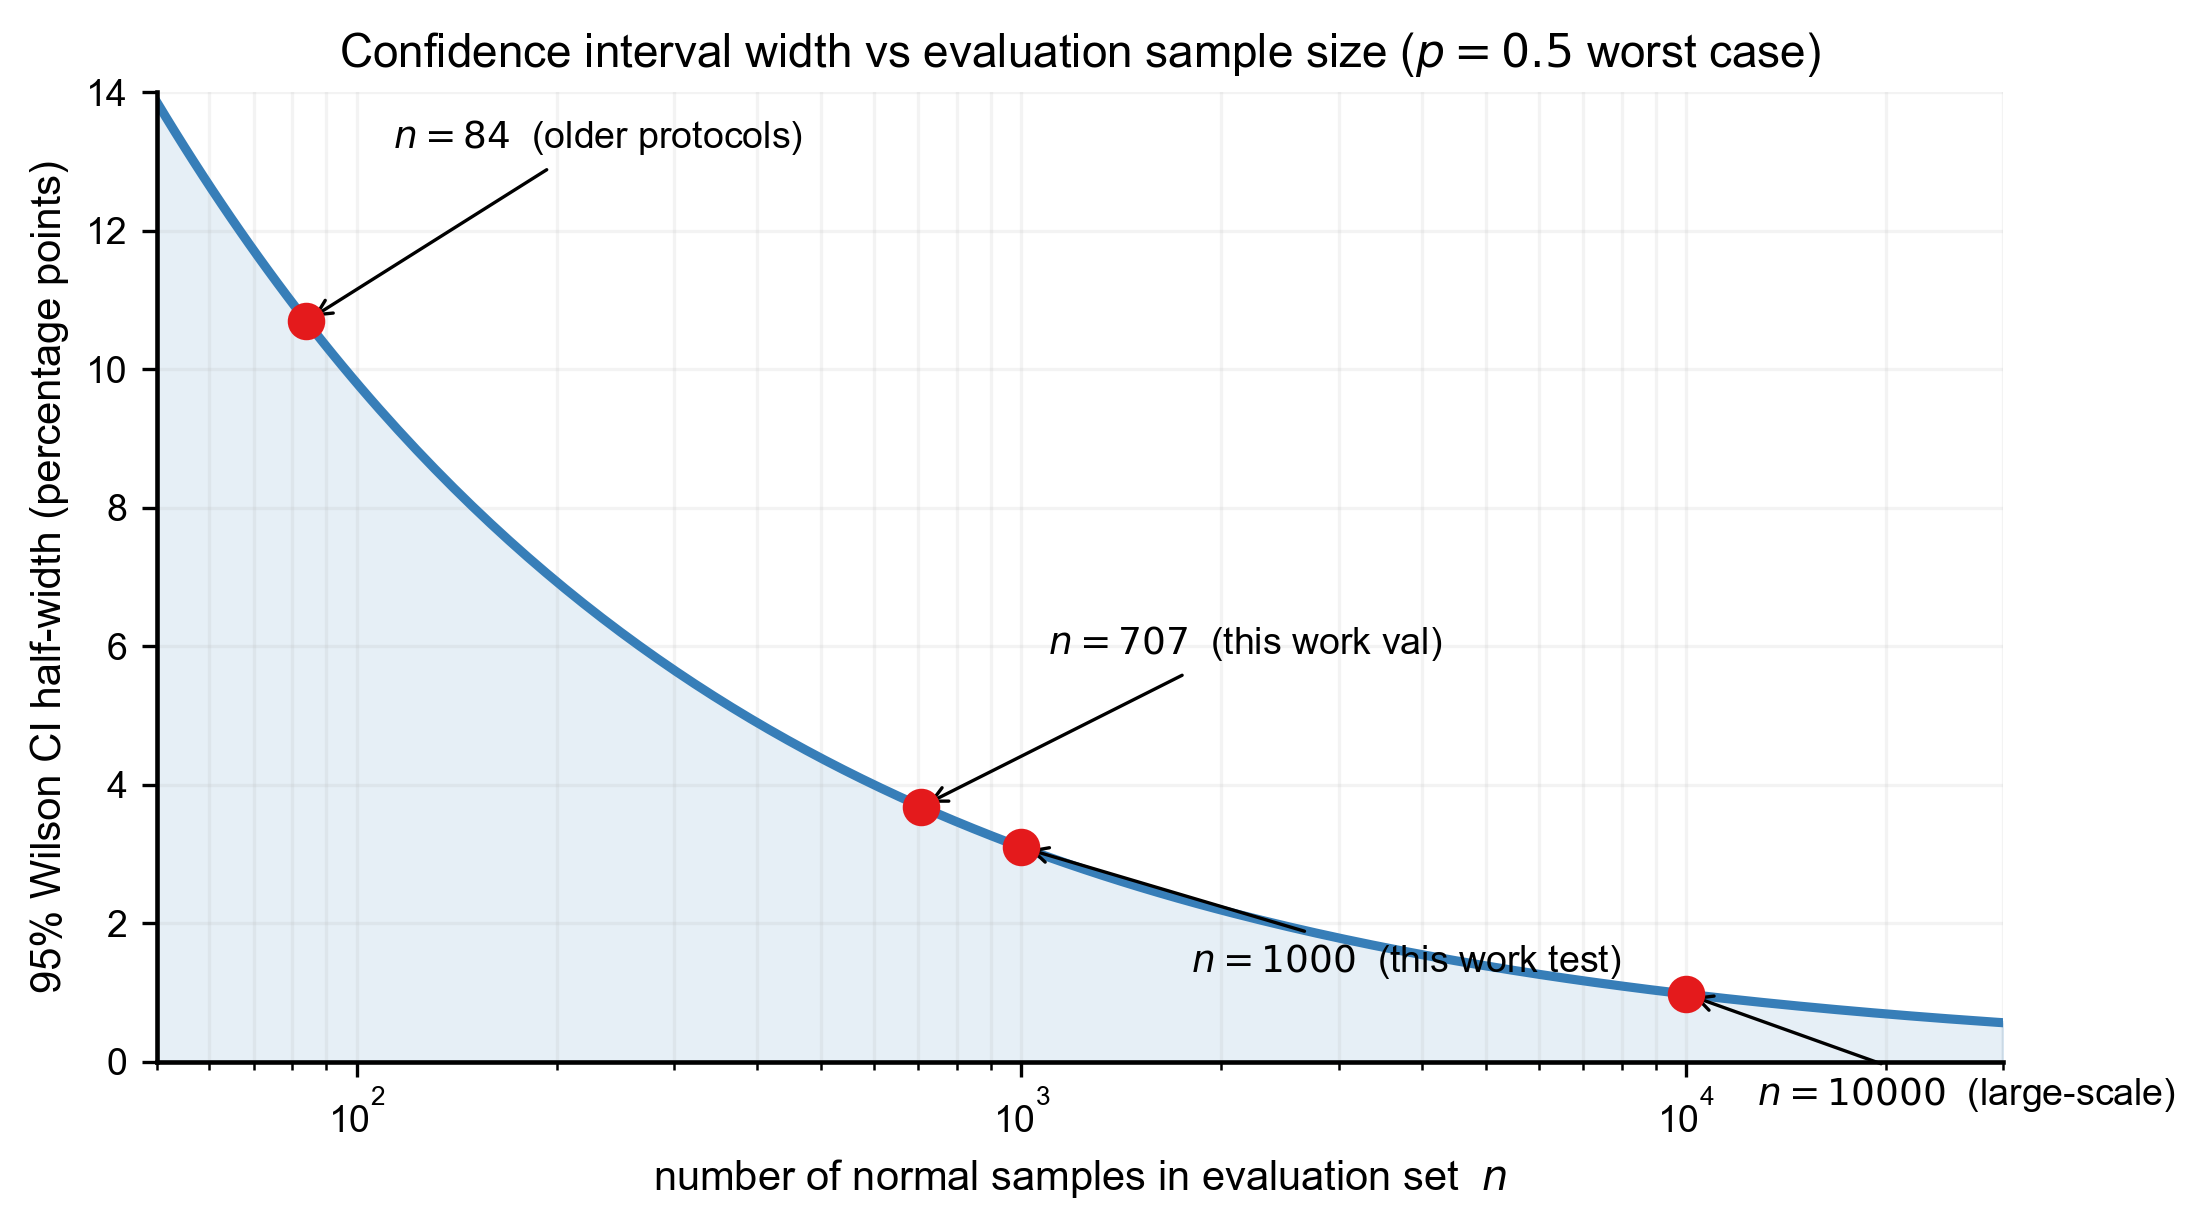
\includegraphics[width=0.82\textwidth]{ch2_wilson_ci_vs_n.png}
    \caption{\textbf{[Wilson 公式理论曲线]} 95\% Wilson 置信区间半宽度随评估集规模 $n$ 的变化（$p = 0.5$ 最坏情形）。小样本评估（$n = 84$）下置信区间宽至 $\pm 10$pp，$n = 700$--$1000$ 时收窄至 $\pm 3$pp 以内，$n$ 超过万量级后边际收益迅速下降。本图数值由式~\eqref{eq:wilson-halfwidth} 解析计算得出，用于说明 Wilson 置信区间的 $O(1/\sqrt{n})$ 收敛性质；不是实验结果。}
    \label{fig:ch2-wilson}
\end{figure}

\section{迁移学习与预训练权重}
本文在五种 YOLO11-cls 容量上统一采用 ImageNet 预训练权重\cite{krizhevsky2012imagenet} 作为初始化，并在目标领域数据上微调。Pan 与 Yang\cite{pan2010transfer} 的综述建立了迁移学习的形式化框架；Yosinski 等\cite{yosinski2014transferable} 实证表明，深度网络的低层特征（边缘、纹理）在源任务与目标任务之间高度可迁移，高层特征逐层特化。在排水管道 CCTV 场景下，预训练提供的底层视觉先验显著降低了从零训练的样本需求量，是本文等条件共享协议的前提条件之一。

\chapter{数据集与实验协议}

本章按照\textbf{从数据现实出发}而非\textbf{从方法出发}的次序组织：先剖析 SewerML 原始数据集的构成与来源（3.1），再对齐 CJJ 181-2012 工程规范以确定分类体系（3.2），接着识别数据质量约束与部署现实场景下必须剔除的样本类型（3.3），据此给出采样策略与数据集构建流程（3.4）；随后对划分规模与训练/评估协议做出决策（3.5--3.7），每项决策均回扣第 2 章的理论依据。

\section{SewerML 原始数据集}
\label{sec:dataset-source}

本文的基础数据源为 Haurum 与 Moeslund\cite{haurum2021sewerml} 于 CVPR 2021 上发布的 Sewer-ML 多标签缺陷分类基准数据集。该数据集由丹麦三家水务公司在九年间积累的 CCTV 巡检视频组成，涵盖 75{,}618 段独立管道检测视频、约 130 万张图像帧，所有帧由持证巡检员按照丹麦 Fotomanualen 规范标注（该规范为欧洲 EN 13508-2 的本地化实施）。相较于规模较小的自建数据集（如 Kumar 等\cite{kumar2018cnn} 的数千张图像），Sewer-ML 的规模与标注一致性使其具备作为排水管道视觉识别领域\textbf{公开可复现基准}的条件。

Sewer-ML 标注体系包含 17 个缺陷类别代码（VA、RB、OB、PF、DE、FS、IS、RO、IN、AF、BE、FO、GR、PH、PB、OS、OP）以及两个语义标签（OK 表示不可检测、ND 表示无缺陷），另附 Defect 二分类标签（Defect=1 表示任一缺陷代码触发）与 WaterLevel 水位等级。原始数据按\textbf{管道级}严格划分为 train / val / test 三个不重叠子集，保证同一段管道的所有帧仅出现于一个子集内，避免训练-评估之间的时间序列泄漏。本文仅使用 Sewer-ML 的训练子集（约 104 万张带标签图像）作为采样池，原始 val 与 test 子集暂不参与本文工作（留待跨基准迁移评估时使用）。

\section{CJJ 181-2012 规范对齐}
\label{sec:cjj-mapping}

\subsection{两套规范的缘起与对照}
本文的数据底座与最终的工程落地分属两套独立的缺陷分类体系，一套是中国的 CJJ 181-2012，一套是 Sewer-ML 所依托的丹麦 Fotomanualen。

\textbf{CJJ 181-2012}\cite{cjj181} 由中国住房和城乡建设部颁布，是城镇排水管道闭路电视检测与评估领域的行业规范。它把 17 种常见管道缺陷按工程性质拆成两大类：一类是\textbf{结构性缺陷}，针对管道本体的物理损伤，涵盖破裂、变形、腐蚀、错口、接口材料脱落、脱节、支管暗接、异物穿入、渗漏、起伏十种情形；另一类是\textbf{功能性缺陷}，反映管道运行状态，包括沉积、结垢、障碍物、残墙坝根、树根、浮渣等七种情形。除分类外，CJJ 181 对每种缺陷给出了从 I 级（轻微）到 IV 级（严重）的四级严重度判定准则，工程上一段管道的检测报告必须同时记录缺陷类型、等级与整改建议——这是规范面向\textbf{工程验收}和\textbf{分级养护决策}的功能定位决定的。

\textbf{Sewer-ML}\cite{haurum2021sewerml} 的标注体系则源自丹麦 Fotomanualen，后者是欧洲 EN 13508-2 的本地化实施。与 CJJ 不同，Sewer-ML 从一开始就为\textbf{图像级多标签分类}设计：每一帧 CCTV 图像由持证巡检员标注它包含的缺陷代码（17 个），既不按结构性/功能性分层组织，也不给出严重等级——只记录"这一帧里是否出现此类缺陷"。这种扁平的多标签粒度对机器学习训练非常友好（每帧图像直接对应一个二值标签向量），但舍弃了 CJJ 所关注的分级评估维度。

两套体系虽然组织方式不同，\textbf{在核心缺陷的识别目标上高度重合}——破裂、变形、错口、腐蚀被两边都列为一级关注的结构性损伤，沉积、障碍物、树根则是共同识别的功能性问题。这一重合使得"用 Sewer-ML 的丹麦图像数据训练模型，再把结论对接到中国 CJJ 工程语境"成为可能，但也带来一个具体问题：需要在两套术语之间建立严格映射，不能简单合并或重命名。这也是下一节的主题。

\subsection{规范对齐的必要性}
\label{sec:cjj-mapping-mapping}
Sewer-ML 的 17 类缺陷命名源自丹麦 Fotomanualen，与中国工程实践中使用的《城镇排水管道检测与评估技术规程》（CJJ 181-2012）\cite{cjj181} 存在命名与粒度差异。若直接在论文中使用 Sewer-ML 原始代码（如 RB、OB、PF），与国内工程规范的衔接受阻；若自行重新命名合并，则需对每一类别提供工程合理性证据。本文选择\textbf{严格向 CJJ 181-2012 对齐}的策略：以 CJJ 181 的缺陷定义作为类别命名与合并粒度的唯一权威来源，Sewer-ML 代码仅作为底层数据载体。该策略的直接收益是，数据集构建过程中任何分类决策均可由 CJJ 181 条文直接支撑，审阅者或工程验证方对合并粒度的质疑均可回归规范条文而非方法论主观选择。

\subsection{SewerML 到 CJJ 181-2012 的映射}
CJJ 181-2012 将管道缺陷分为结构性与功能性两大类共 17 种。结合 Sewer-ML 标注体系的可用性、各类在数据集中的样本量，以及本文二分类门控任务对\textbf{异常帧的统一标识}的需求，本文选取覆盖 CJJ 主要缺陷且与 Sewer-ML 代码一一对应的\textbf{6 类缺陷 + 1 类正常}作为分类体系。表~\ref{tab:sewerml-cjj-mapping} 给出完整映射。

\begin{table}[H]
    \centering
    \caption{SewerML 代码到 CJJ 181-2012 缺陷类别的严格映射}
    \label{tab:sewerml-cjj-mapping}
    \begin{tabularx}{\textwidth}{p{2.6cm}p{2.2cm}p{2.0cm}X}
        \toprule
        CJJ 类别 & 代码 & SewerML 代码 & 本文处理 \\
        \midrule
        正常                  & ---   & Defect=0  & 二分类负类 \\
        破裂                  & PL    & PF        & 二分类正类 \\
        变形                  & BX    & DE        & 二分类正类 \\
        错口                  & CK    & FS        & 二分类正类 \\
        腐蚀                  & FS    & RB        & 二分类正类 \\
        沉积                  & CJ    & AF        & 二分类正类 \\
        障碍物                & ZW    & OB        & 二分类正类 \\
        \midrule
        图像质量问题          & ---   & OK, PH    & 数据质量剔除（见 3.3） \\
        其他                  & ---   & BE, RO, IN, FO, GR, PB, OS, OP, VA & 不纳入本文范围 \\
        \bottomrule
    \end{tabularx}
\end{table}

正常帧作为二分类门控的负类基底，呈现均匀过渡的灰色或浅黄色管壁，管节接缝以规整的圆环状明暗分界位于画面深处，没有局部反差或几何突变。本文纳入的六类缺陷按物理成因可归入三组：管体自身的结构性损伤（破裂、变形、错口）、管壁材料表层的化学与生物劣化（腐蚀），以及外来物质在管内的堆积（沉积、障碍物）；每一类的视觉形态由其成因机制与在管道截面中发生的空间位置共同决定，门控分类器在不同类别上可利用的视觉线索因此显著不同。下文按"外来前景—结构整体—结构局部—表层纹理—管底堆积"的顺序依次介绍。

\begin{figure}[H]
    \centering
    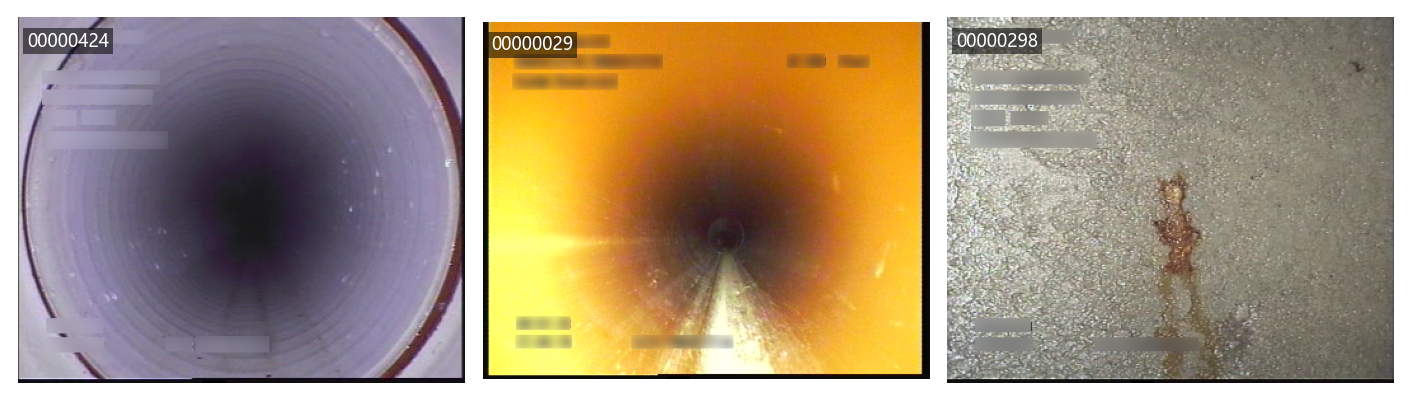
\includegraphics[width=0.85\textwidth]{ch3_class_normal.png}
    \caption{Sewer-ML 中的正常管道画面。}
    \label{fig:ch3-cls-normal}
\end{figure}

障碍物（ZW/OB）由施工残留的石块与钢筋、经井口冲入的生活垃圾、上游管段脱落的构件等异源物质进入管内形成，其存在与管道本体的结构状态无直接因果关联。反映在画面中，障碍物表现为边界清晰的高对比度前景物体，位置不定、形态各异；由于外来物来源多样，其几何与材质差异构成了六类缺陷中最高的类内视觉方差。

\begin{figure}[H]
    \centering
    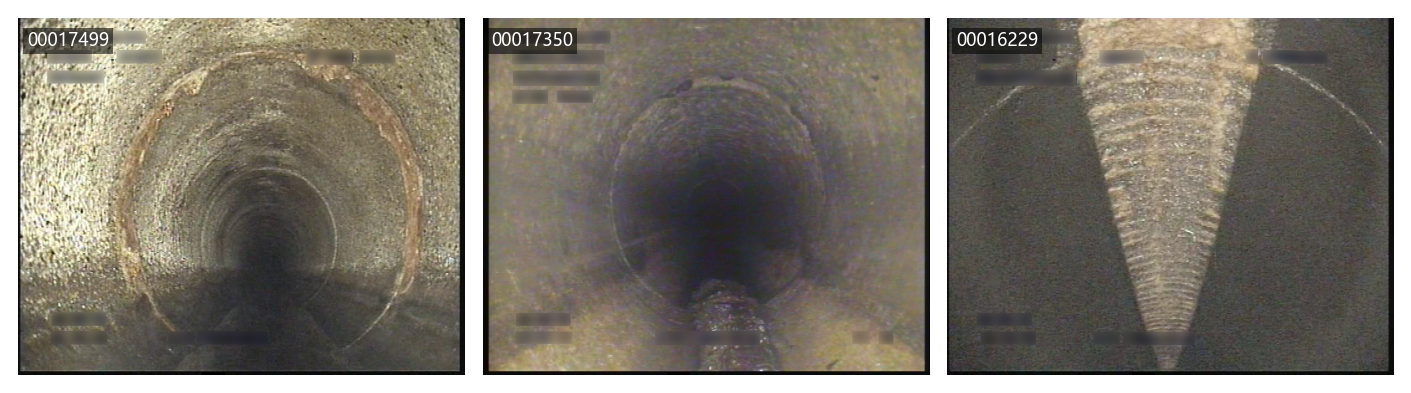
\includegraphics[width=0.85\textwidth]{ch3_class_obstacle.png}
    \caption{障碍物 ZW（对应 Sewer-ML 代码 OB）。}
    \label{fig:ch3-cls-obstacle}
\end{figure}

变形（BX/DE）的物理成因是地面车辆荷载、回填土不均匀压力或地基沉降导致管道截面从圆形向椭圆、多边形乃至不规则形状过渡，是长期外部应力累积的结果。其视觉线索不在前景而在结构：管道本应圆形的轮廓在画面深处被压扁、鼓出或呈椭圆，识别依赖画面远端管口的整体几何形状而非任一局部细节。这一"整体形状而非局部纹理"的判读方式使其在视觉上与其他局部型缺陷显著不同。

\begin{figure}[H]
    \centering
    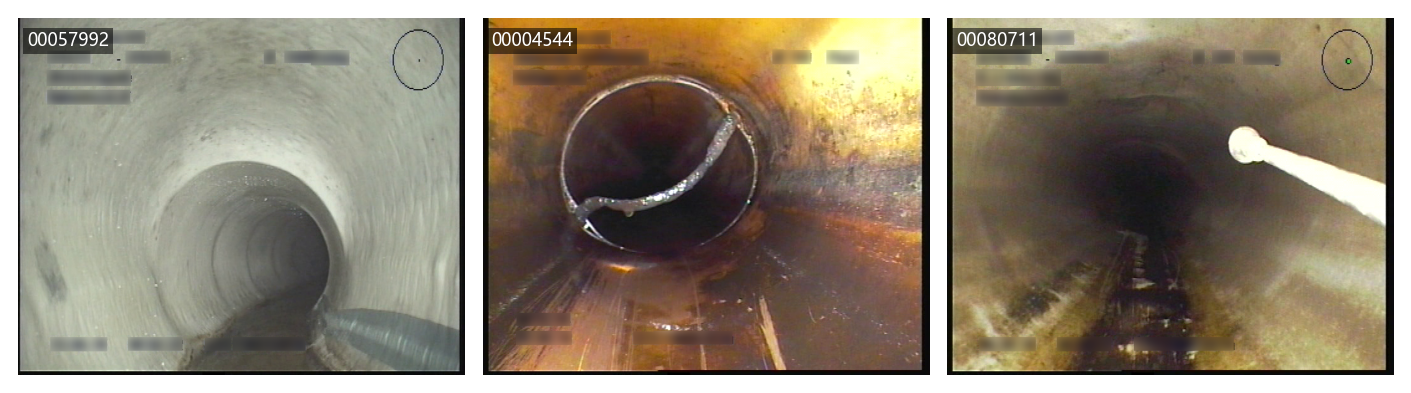
\includegraphics[width=0.85\textwidth]{ch3_class_deformation.png}
    \caption{变形 BX（对应 Sewer-ML 代码 DE）。}
    \label{fig:ch3-cls-deformation}
\end{figure}

破裂（PL/PF）由管壁在长期内外压、温度胀缩、冲击荷载或材料疲劳作用下的物理开裂产生，是管道结构性失效最直接的视觉证据。画面上呈线状或条状黑色缝隙，可沿管轴纵向延伸或环向横切，粗细差异较大，但共同视觉特征为高对比度的细长形状。与变形依赖整体轮廓不同，破裂的视觉信息集中在画面中某一局部，且该局部的信号强度显著高于正常管壁的纹理水平。

\begin{figure}[H]
    \centering
    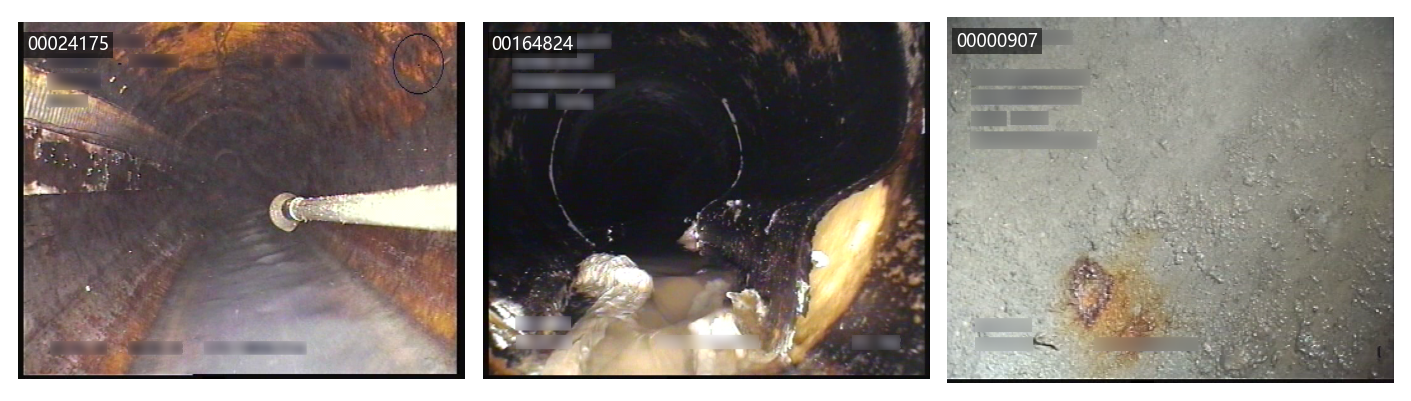
\includegraphics[width=0.85\textwidth]{ch3_class_break.png}
    \caption{破裂 PL（对应 Sewer-ML 代码 PF）。}
    \label{fig:ch3-cls-break}
\end{figure}

错口（CK/FS）由相邻管节在地基不均匀沉降、施工对中误差或地下土体位移作用下沿轴线方向发生错位形成，位置严格约束在两段管节的接缝处。错口与破裂同属局部高对比特征，但位置高度规律：管节接缝本身在 CCTV 远景中即为一条圆环状明暗分界，错口表现为该分界上的可见台阶，对应上下游管段中轴线错位的几何结果。

\begin{figure}[H]
    \centering
    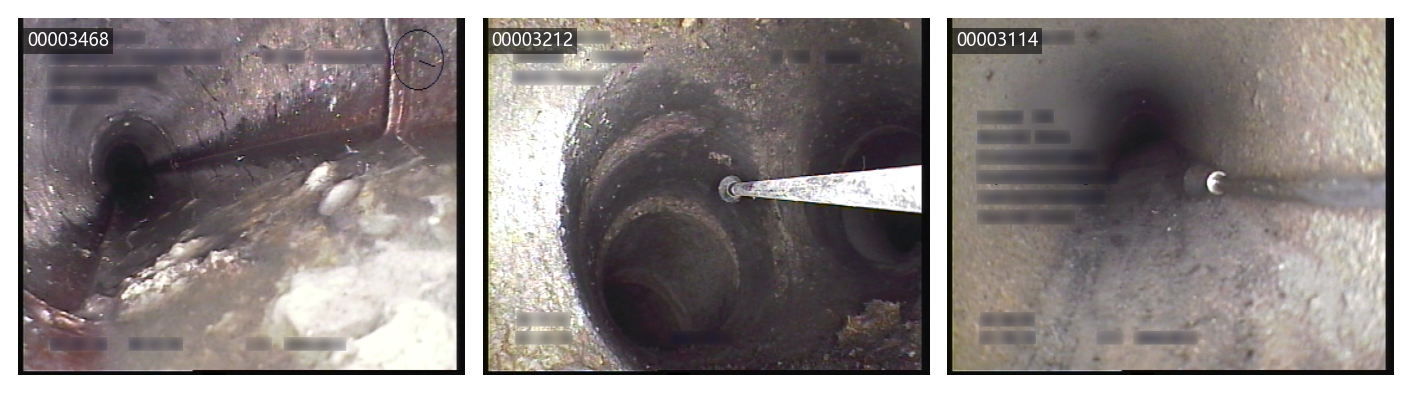
\includegraphics[width=0.85\textwidth]{ch3_class_dislocation.png}
    \caption{错口 CK（对应 Sewer-ML 代码 FS）。}
    \label{fig:ch3-cls-dislocation}
\end{figure}

腐蚀（FS/RB）由排水介质中的硫化氢、酸性排放物以及长期湿润环境对混凝土与金属管壁的化学与生物劣化持续累积形成，作用范围覆盖整段管壁而非某一局部。画面上呈面状低频的纹理变化：整段管壁表面粗糙化，麻点密布，色调从原色向黄褐黑漂移。与破裂、错口的地标式特征不同，腐蚀的识别依赖对整片管壁纹理的统计比较，在弱光或远景帧中的可分辨性较低。

\begin{figure}[H]
    \centering
    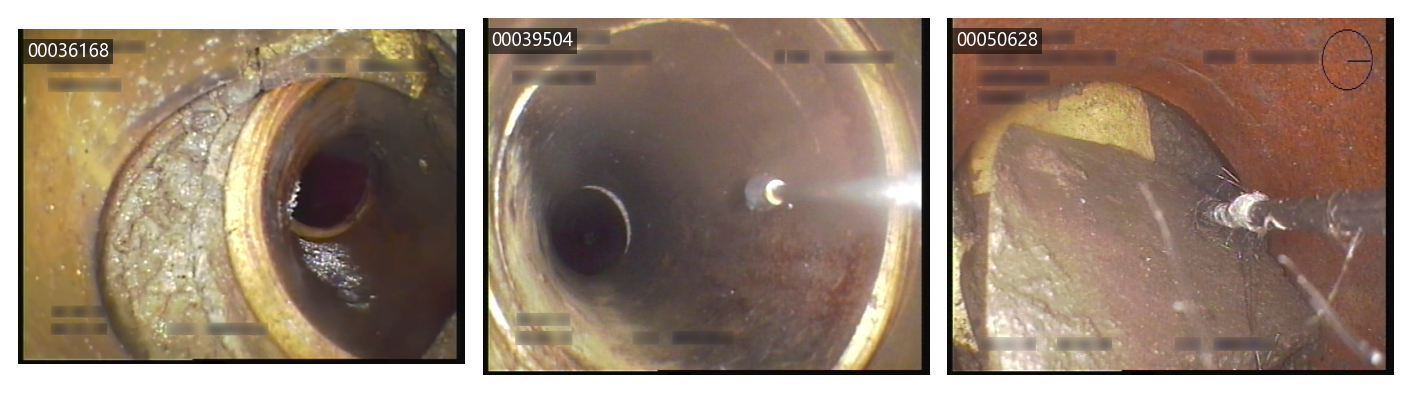
\includegraphics[width=0.85\textwidth]{ch3_class_corrosion.png}
    \caption{腐蚀 FS（对应 Sewer-ML 代码 RB）。}
    \label{fig:ch3-cls-corrosion}
\end{figure}

沉积（CJ/AF）由流速不足、管道坡度不当或污水中泥沙垃圾在管底长期沉降积累形成，与管道本体的几何和表层均无直接关联，是管道功能性失效的典型表现。画面下缘通常覆盖灰白、泥黄或褐色堆积层并向远端延伸；堆积厚度较大时，下半部分管壁轮廓被抬起，在画面远端与变形引起的几何畸变在视觉上存在一定重叠。

\begin{figure}[H]
    \centering
    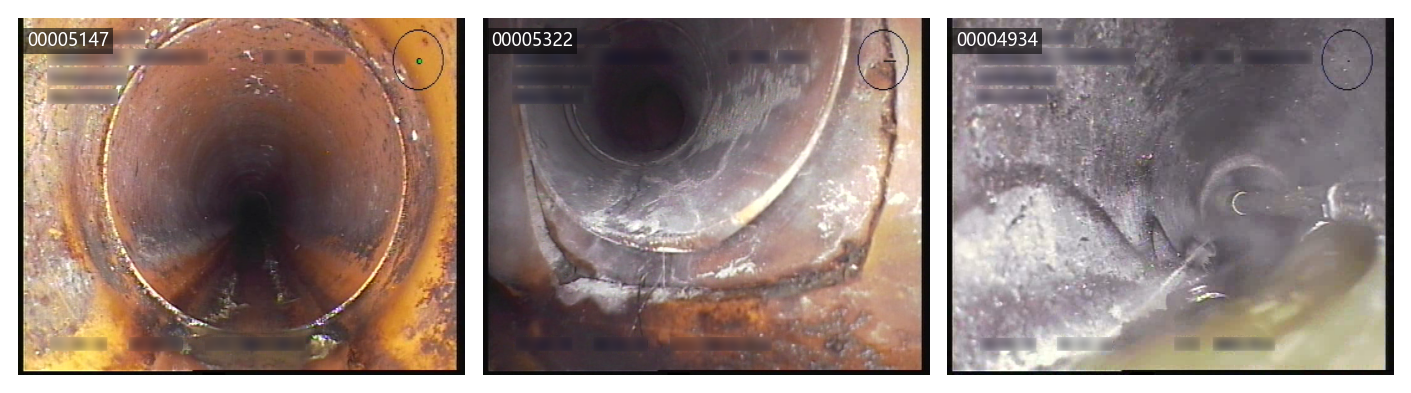
\includegraphics[width=0.85\textwidth]{ch3_class_deposit.png}
    \caption{沉积 CJ（对应 Sewer-ML 代码 AF）。}
    \label{fig:ch3-cls-deposit}
\end{figure}

映射过程遵循两项严格约束。其一，\textbf{不跨 CJJ 类别合并}：即使 Sewer-ML 的 AF（附着沉积）与 BE（结垢）在视觉上相近，也不合并为单一类别，因 CJJ 181-2012 明确区分沉积（CJ）与结垢（JG）；合并会造成规范术语混淆。该约束意味着 BE 仅能作为 holdout，不进入训练任务。其二，\textbf{holdout 类不参与训练但保留数据集内}：树根、渗漏、结垢、起伏在 Sewer-ML 中存在样本但数量稀少或定义边界模糊，不纳入本文 6 类主任务，但在采样时不因其标签存在而排除对应图像——该图像若同时具有主任务类别（多标签情形），仍以主任务类别归入二分类正类；若仅具 holdout 类别，则从采样池中排除。该约束保留了未来扩展到 7 类或 8 类任务的数据延展性。

\subsection{二分类门控视图下的标签简化}
本章构建的数据集支持后续可能的 6 类精细分类研究（如第二阶段检测任务），但本文所关注的第一阶段门控仅做二分类决策。二分类视图下，标签函数定义为
\begin{equation}
y(x) = \begin{cases}
0, & \text{若 } x \text{ 不具备任一主任务缺陷代码}, \\
1, & \text{若 } x \text{ 具备 PF、DE、FS、RB、AF、OB 中任一代码}.
\end{cases}
\label{eq:binary-label}
\end{equation}
式~\eqref{eq:binary-label} 将 6 类缺陷合并为统一的 \emph{Abnormal}（$y = 1$）类，与 CJJ 181 的"任何结构或功能性缺陷均需进入后续评估"的工程判读逻辑一致。

\section{数据质量约束与部署现实}
\label{sec:quality-constraints}

Sewer-ML 中的 OK 与 PH 两个标签对应\textbf{采集过程的失败}而非管道本身的缺陷：OK 表示画面模糊、水位过高或镜头脏污导致的不可检测帧，PH 表示摄影缺陷（曝光异常、失焦、色彩畸变等）。在实际 CCTV 部署链路中，这两类帧应由\textbf{预处理阶段的图像质量过滤模块}剔除（工程上常见为基于 Laplacian 方差的模糊检测与基于亮度直方图的曝光异常检测），不应进入门控分类器的判别范围。

本文将 OK 与 PH 作为\textbf{数据质量不合格帧}从训练、验证与测试集中统一剔除，理由如下：

\textbf{其一，语义不匹配}。门控分类器的任务是判断"管道是否存在缺陷"；OK/PH 帧上没有足够信息支持这一判断，强迫分类器学习 OK/PH 帧上的模式不仅没有工程意义，反而会将"画质异常"的视觉特征错误绑定到"存在缺陷"或"不存在缺陷"的决策空间上。

\textbf{其二，评估噪声放大}。若将 OK/PH 帧纳入评估集，模型在这些帧上的预测表现无法被真实标签（正常/异常）有意义地检验——OK 帧本身就不可判读，ND 或 Defect 的标注在 OK 存在时并不可靠。这会导致 Spec 与 Recall 的估计引入系统性噪声。

\textbf{其三，与部署链路一致}。实际巡检系统中，OK/PH 帧在 Stage 0 质量过滤后即被标记为"待重测"，不会进入后续分类或检测模块。本文剔除 OK/PH 的协议与这一部署链路完全一致，保证实验结论可直接迁移到部署场景。

本文将图像质量过滤视作\textbf{独立的前置模块}，不作为本文方法的一部分展开，仅在数据集构建时统一剔除 OK 与 PH 标签触发的所有帧。剔除规则为：若图像 $x$ 满足 $\mathbb{1}[\mathrm{OK}(x)] = 1$ 或 $\mathbb{1}[\mathrm{PH}(x)] = 1$，则 $x$ 不进入采样池，无论其是否同时具备其他缺陷标签。

\section{采样与数据集构建}
\label{sec:sampling}

\subsection{采样池的形成}
以 Sewer-ML 训练子集的约 104 万张图像为起点，经下列三步过滤形成本文采样池：（1）剔除 OK 与 PH 帧（见 \ref{sec:quality-constraints}）；（2）剔除 holdout 类别独占帧（仅具 BE、RO、IN、FO 标签且不具备任何主任务类别的帧）；（3）确认剩余帧的 Defect 标签与主任务类别标签的一致性，丢弃少量标签冲突的边缘样本。图~\ref{fig:ch3-funnel} 给出完整的构建漏斗。

\begin{figure}[H]
    \centering
    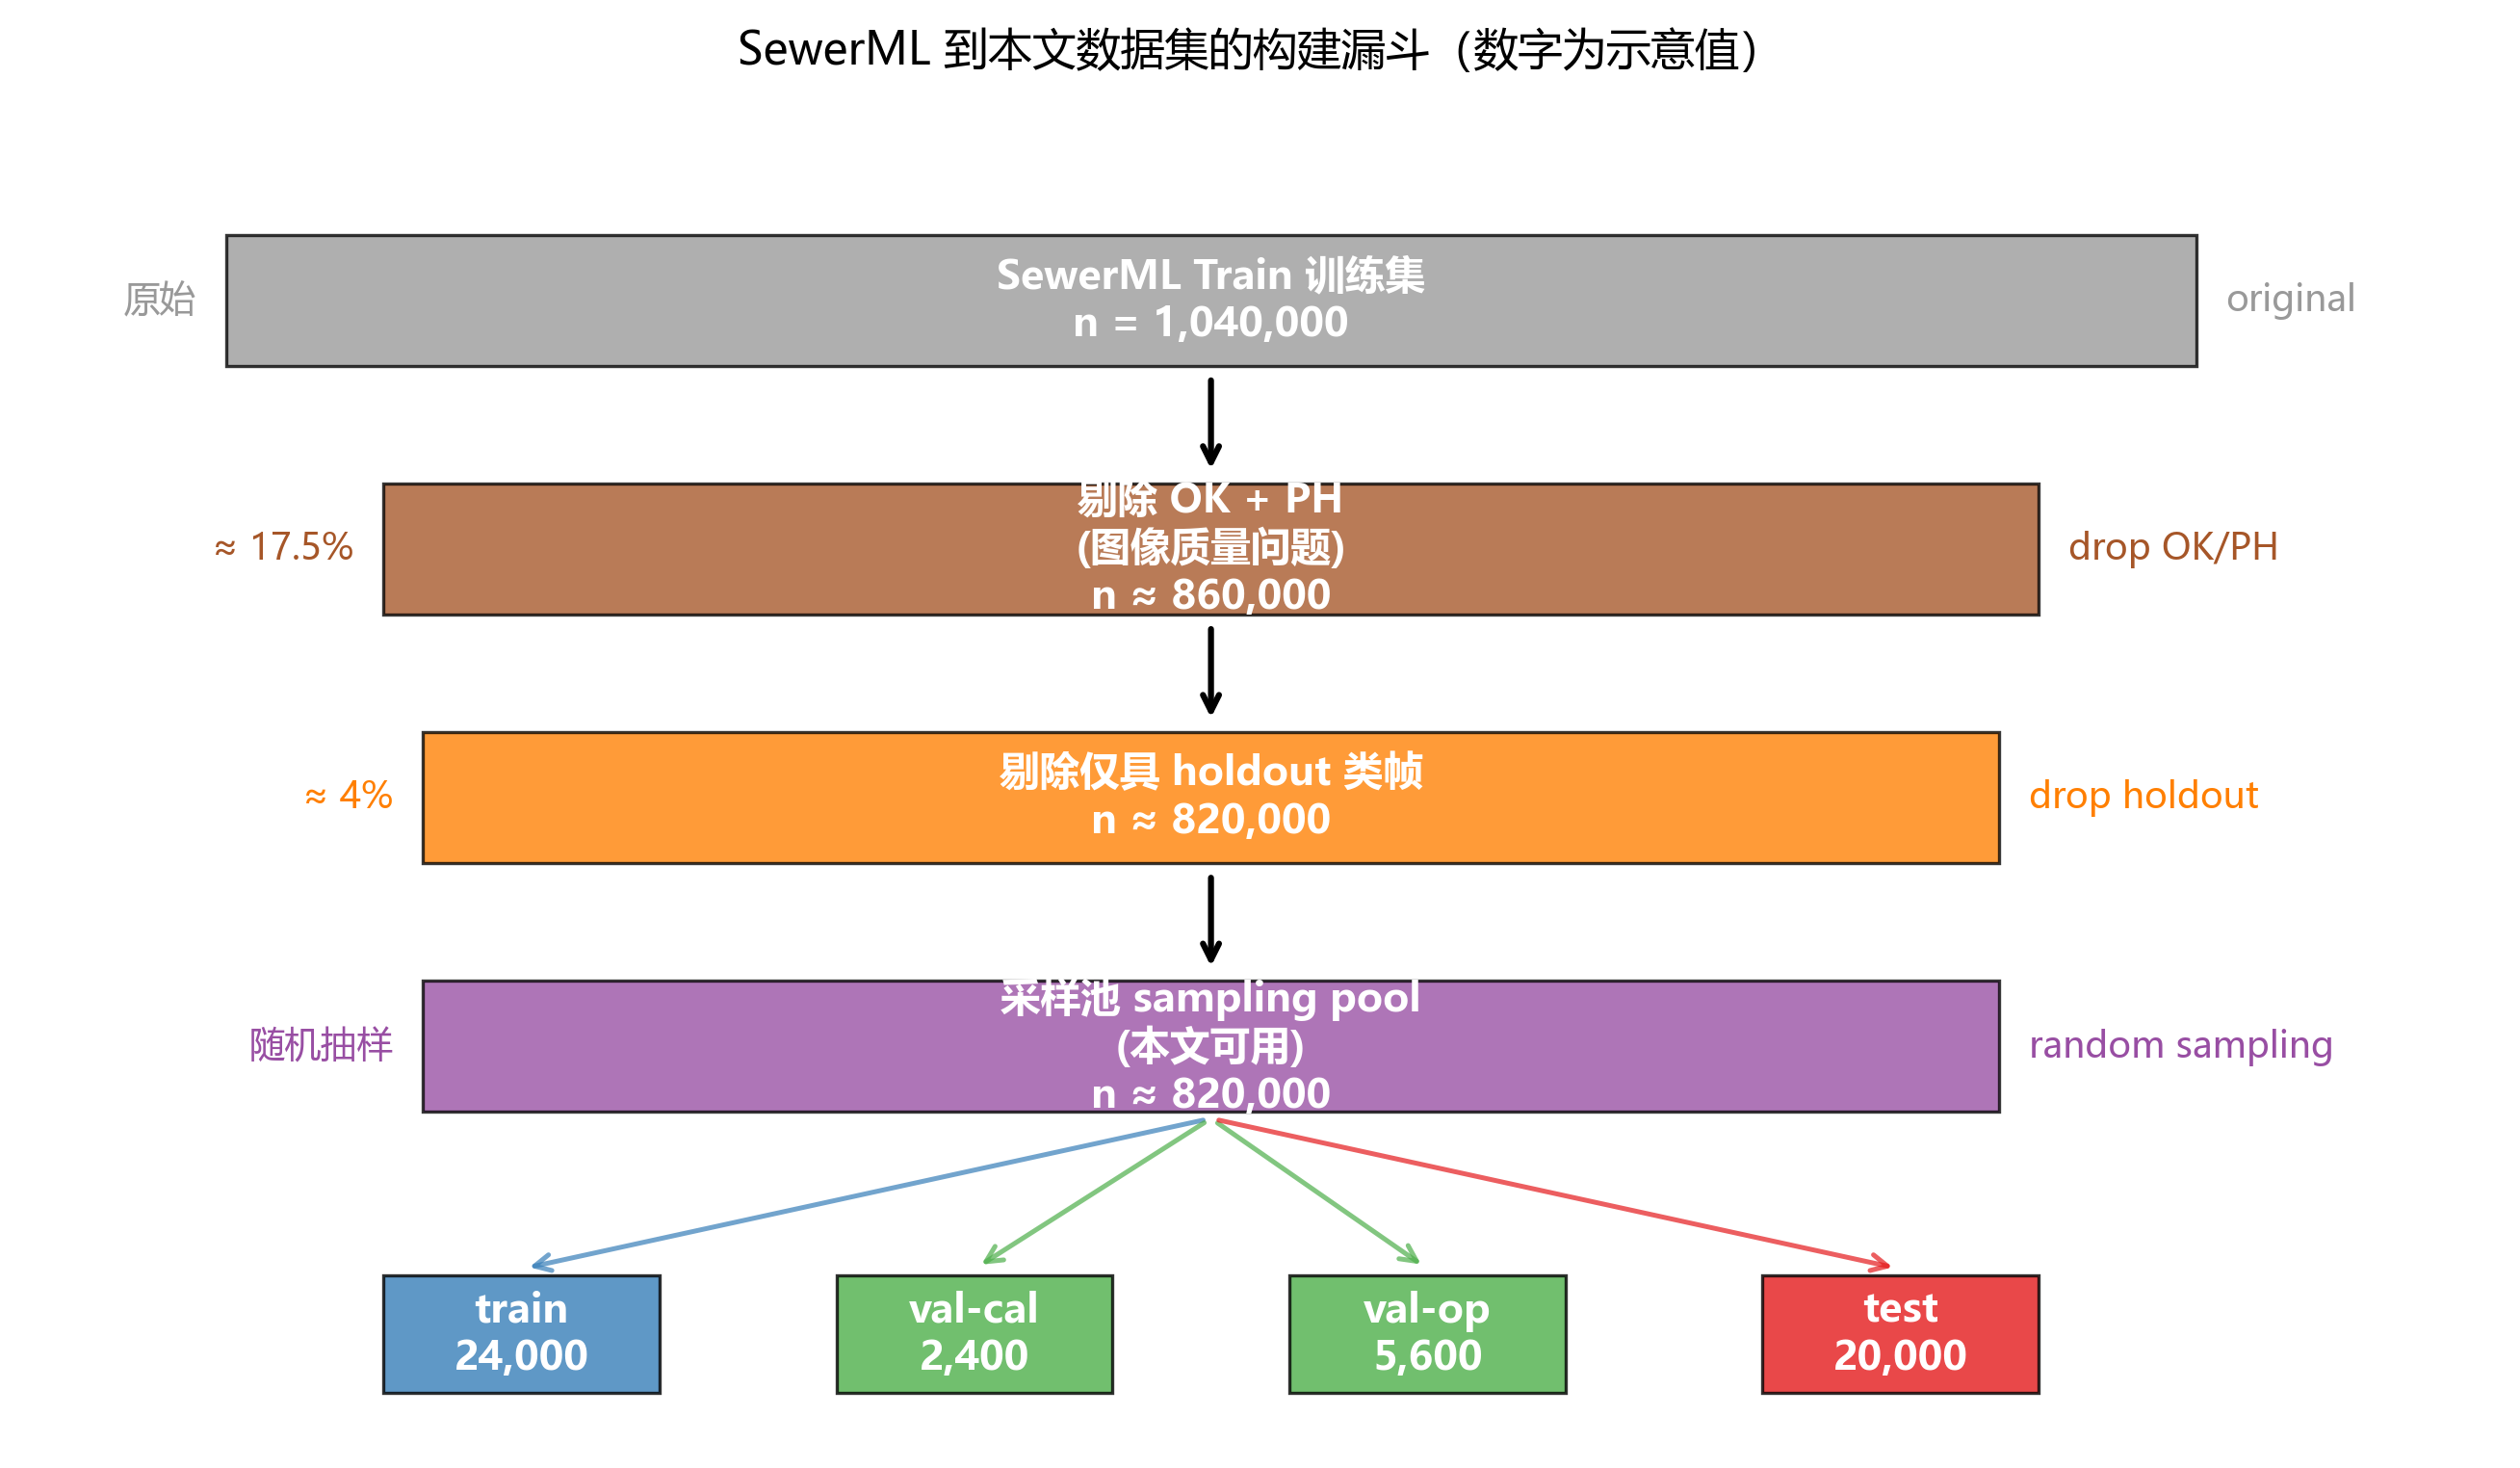
\includegraphics[width=\textwidth]{ch3_data_funnel.png}
    \caption{\textbf{[数据集构建流程示意图]} 从 Sewer-ML 原始训练集到本文采样池的过滤漏斗，以及进一步划分为 train/val-cal/val-op/test 四个子集的结构。各子集规模为研究设计目标值，确定依据见 \ref{sec:split-sizes} 节。}
    \label{fig:ch3-funnel}
\end{figure}

过滤后，采样池包含约 80--90 万张\textbf{可直接用于本文二分类任务}的图像。其中正常帧（Defect=0）占比较高，符合真实排水管道巡检中正常帧远多于缺陷帧的分布\cite{haurum2020survey}。图~\ref{fig:ch3-distribution} 给出 CJJ 6 类缺陷在 Sewer-ML 训练集中的自然分布：正常类最多（约 55 万），其次是错口、障碍物、沉积，破裂与变形相对稀少。本文在采样时不人为校正这一自然分布，使训练与评估集均保持与真实巡检场景一致的先验结构。

\begin{figure}[H]
    \centering
    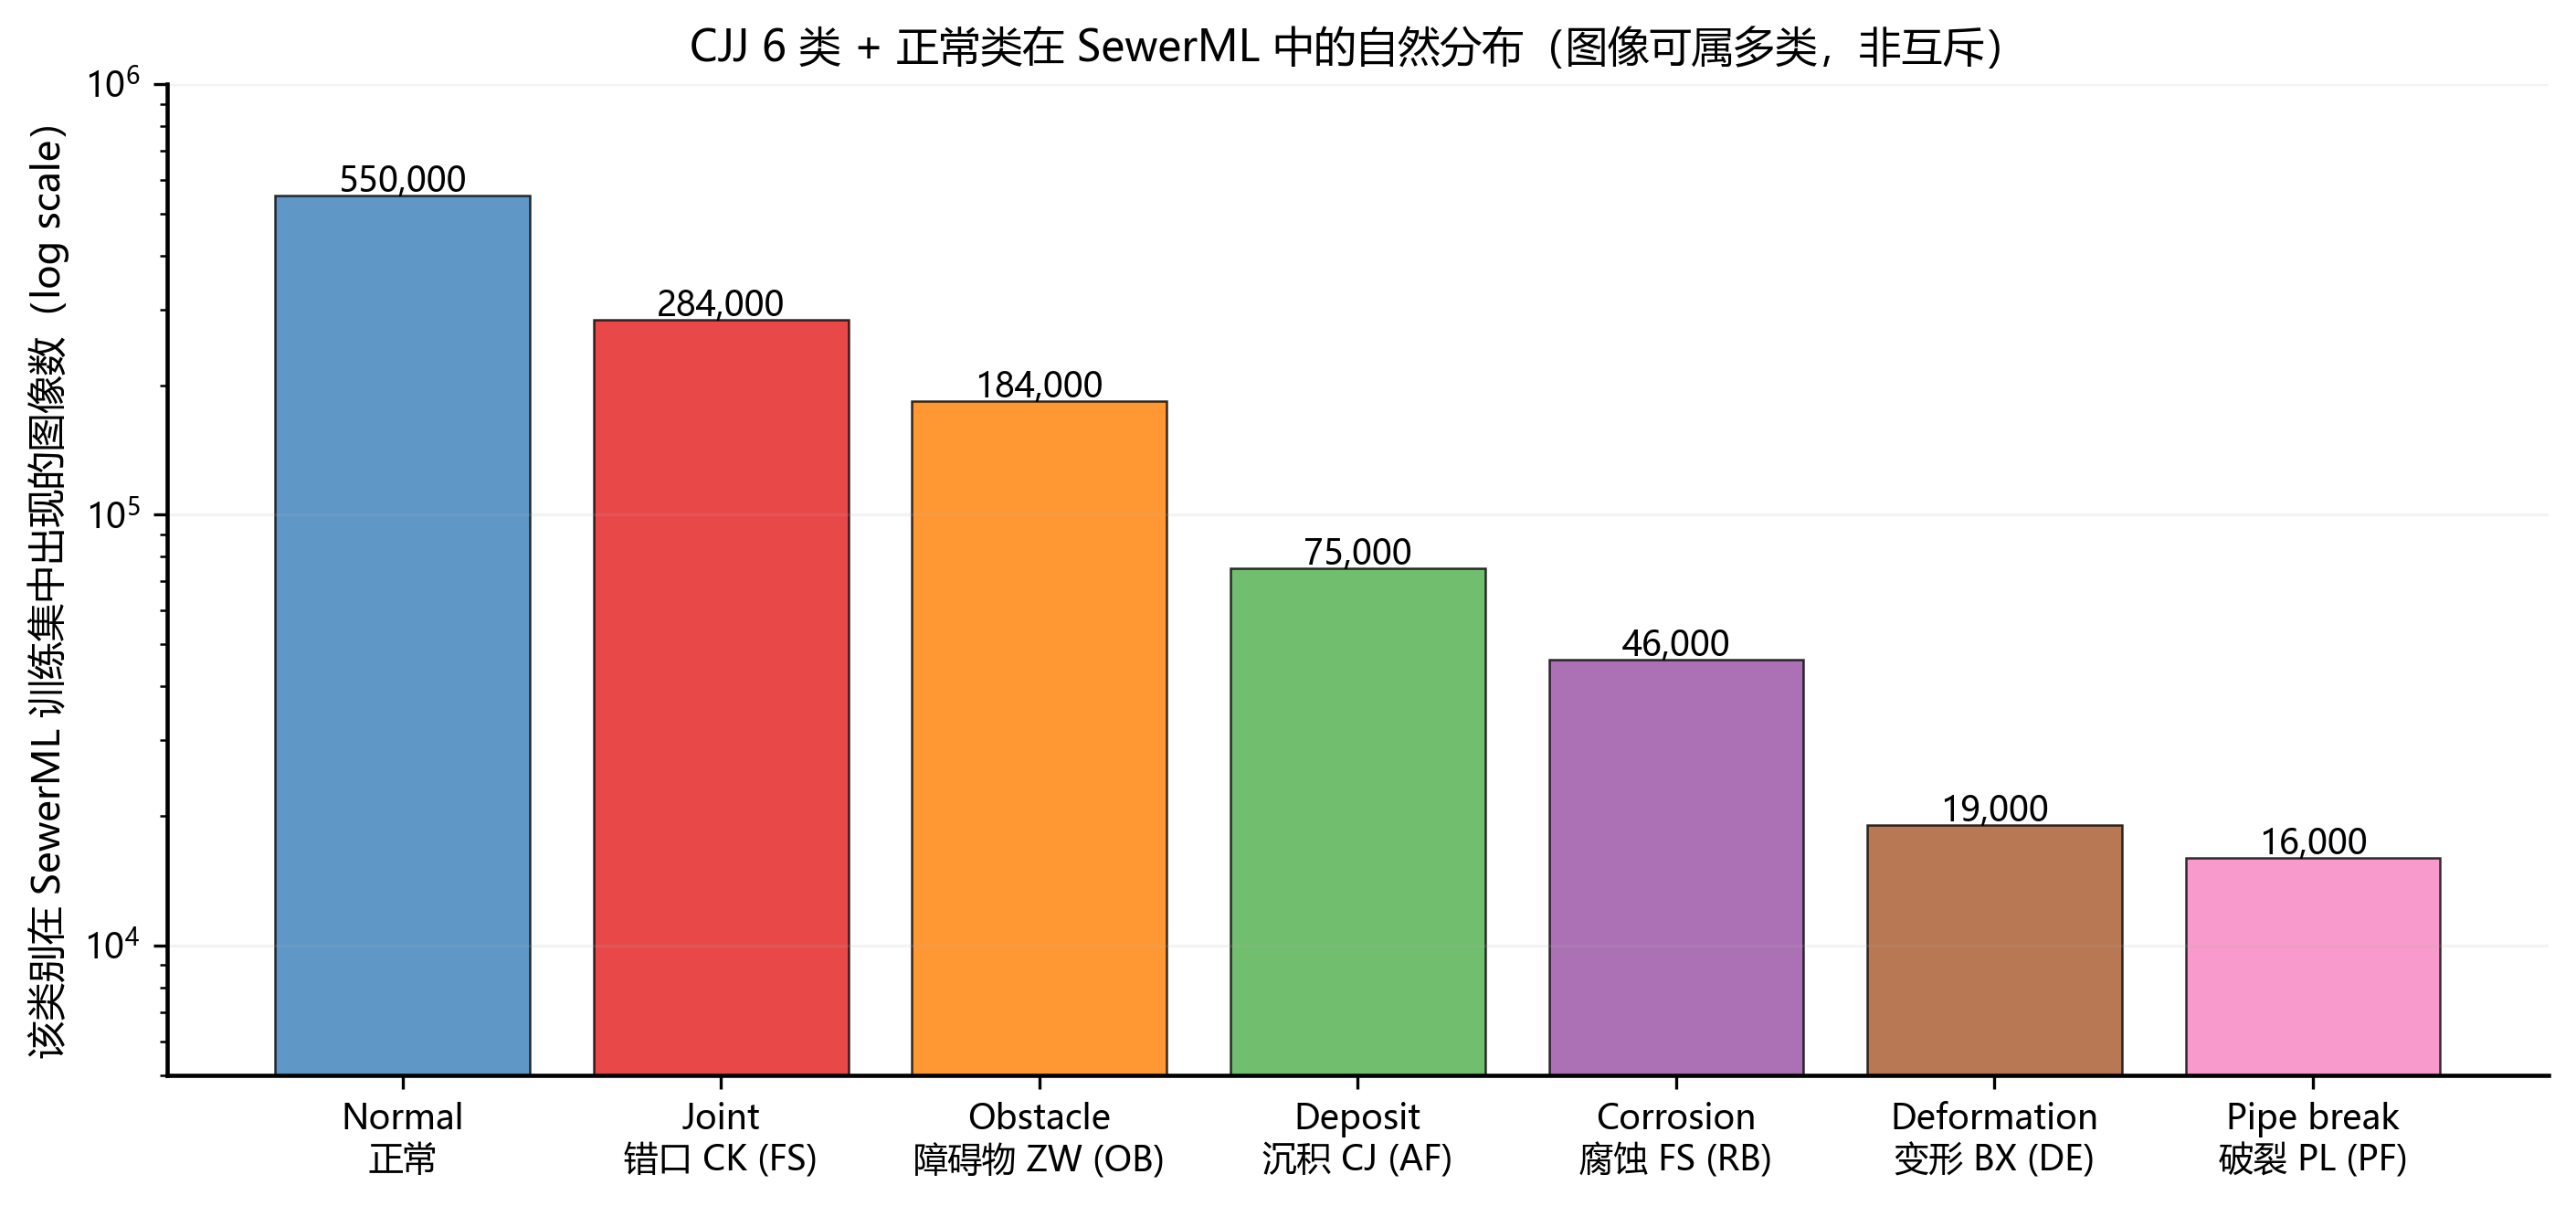
\includegraphics[width=\textwidth]{ch3_cjj_distribution.png}
    \caption{\textbf{[SewerML 数据集标注统计]} CJJ 6 类 + 正常类在 Sewer-ML 训练集中的自然分布（对数纵轴）。图像可同时具备多类标签，柱状图反映的是每类触发次数而非互斥类占比。错口、障碍物两类出现频率最高，破裂与变形相对稀少——与 CJJ 工程经验中"结构性缺陷频率低于功能性缺陷"的一般观察一致。本图由 Sewer-ML 公开标注 CSV 直接统计得出，属数据集客观属性，任何按相同 CJJ 映射规则的独立统计均可复现该结果；不包含本文训练或评估产生的数据。}
    \label{fig:ch3-distribution}
\end{figure}

\subsection{多标签保留与真实分布}
与部分现有工作\cite{kumar2018cnn} 将数据集过滤为\textbf{单标签}以简化分类任务的做法不同，本文在采样时\textbf{不排除多标签帧}：若某帧同时具备破裂（PF）与障碍物（OB）两种标签，在二分类视图下按式~\eqref{eq:binary-label} 判为 $y = 1$，该帧仍进入采样池。理由为：

真实管道中不同类型缺陷共存是常态——管道老化过程中破裂往往伴随变形、腐蚀与附着沉积，新接入支管可能同时伴随错口与障碍物。强制单标签采样会系统性地排除这些"更典型的部署场景样本"，使训练得到的模型在多缺陷共存帧上泛化能力下降。本文保留多标签帧的做法与 Sewer-ML 原始基准\cite{haurum2021sewerml} 的多标签定位一致，使得训练集的缺陷共存分布贴近真实部署。

保留多标签帧的同时需要防范\textbf{任务定义污染}：当一张帧的主任务类（如 PF 破裂）仅为次要视觉内容，而 holdout 类（如 BE 结垢）在画面中视觉主导时，二分类门控若简单将其判为 $y = 1$，事实上可能学到"结垢 = 异常"的判别面而非"破裂 = 异常"，在纯净单类帧上的泛化将因此下降。本文不对"视觉主导"做主观删选（该判定不可复现），而采取显式披露策略：附录将给出 $\mathcal{D}_{\rm train}$、$\mathcal{D}_{\rm val}$、$\mathcal{D}_{\rm test}$ 各自的\textbf{"主任务类 $\times$ holdout 类"共现矩阵}与多标签帧占比；若后续章节发现 per-class recall 在某一稀少主任务类上异常偏低，将在结果讨论中回溯至该共现矩阵进行归因。

\subsection{采样流程}
本文采用随机采样（uniform random sampling）从采样池中抽取训练、验证与测试集。\textbf{采样种子固定}为 20260417，保证数据集构建可重现。采样过程为一次性完成：先抽取训练集所需样本数，再从剩余池中抽取验证集，最后从再剩余池中抽取测试集，三者逻辑上严格不重叠。该一次性采样流程相较于"先合并采样再划分"的做法具备两项优势：其一，避免划分边界上的数据泄漏风险；其二，便于在不同规模实验中扩展训练集而不影响既有验证与测试集的独立性。

\section{数据集划分与规模决策}
\label{sec:split-sizes}

本文将数据集划分为三个\textbf{严格不重叠}的子集：训练集 $\mathcal{D}_{\rm train}$、验证集 $\mathcal{D}_{\rm val}$ 与测试集 $\mathcal{D}_{\rm test}$，其中验证集进一步二次划分为校准子集 $\mathcal{D}_{\rm val\text{-}cal}$ 与工作点评估子集 $\mathcal{D}_{\rm val\text{-}op}$。表~\ref{tab:dataset-sizes} 汇总各子集规模与用途。

\begin{table}[H]
    \centering
    \caption{数据集子集划分、规模与用途}
    \label{tab:dataset-sizes}
    \begin{tabularx}{\textwidth}{p{2.6cm}p{2.2cm}X}
        \toprule
        子集 & 规模（约） & 用途 \\
        \midrule
        $\mathcal{D}_{\rm train}$    & 24{,}000 张 & 训练五容量 YOLO11-cls 骨干 \\
        $\mathcal{D}_{\rm val\text{-}cal}$ & 2{,}400 张 ($\approx$ val $\times$ 30\%)  & 拟合温度 $T$（式~\eqref{eq:temperature-nll}）\\
        $\mathcal{D}_{\rm val\text{-}op}$  & 5{,}600 张 ($\approx$ val $\times$ 70\%)  & 搜索阈值 $\tau_{R_0}$（式~\eqref{eq:constrained-threshold}）、选最优检查点 \\
        $\mathcal{D}_{\rm test}$     & 20{,}000 张 & 最终指标报告（仅用一次） \\
        \bottomrule
    \end{tabularx}
\end{table}

\subsection{训练集规模的决策}
训练集规模 24{,}000 张的选择基于三项可溯源的约束——采样覆盖、迁移学习规模规律与计算预算——共同构成的可行区间。

\textbf{约束一：采样覆盖的下界}。图~\ref{fig:ch3-distribution} 显示 CJJ 6 类中破裂（PF）与变形（DE）两类在 Sewer-ML 训练集中相对稀少，各约 1--2 万张。若按本文 \ref{sec:sampling} 节的随机采样策略不做类别均衡，则训练集规模 $n_{\rm train}$ 中这两类的期望样本数为 $n_{\rm train} \cdot p_c$，其中 $p_c$ 为该类在采样池中的占比（约 2\%）。为使破裂与变形两类在训练集中至少各出现若干百张（保证模型能学到基本视觉模式而非完全缺失），应有
\begin{equation}
n_{\rm train} \cdot p_{\rm PF} \geq 300 \;\Rightarrow\; n_{\rm train} \geq 300 / 0.02 = 15{,}000.
\label{eq:train-lowerbound}
\end{equation}
即训练集下界不应低于约 1.5 万。

\textbf{约束二：迁移学习规模规律的上界提示}。Hestness 等\cite{hestness2017scaling} 通过跨领域实证发现，在固定模型架构下，测试误差与训练样本量近似服从幂律下降：$\varepsilon(n) \sim \alpha + \beta n^{-\gamma}$，其中图像分类任务上 $\gamma$ 的实测范围约为 0.07--0.35。Sun 等\cite{sun2017revisiting} 在 JFT-300M 上的大规模实证进一步支持了视觉识别任务中性能随训练数据呈对数线性增长的规律——这一规律意味着从 $n = 10^4$ 扩大到 $n = 10^5$ 所能带来的性能提升并非数量级改善。在迁移学习的具体场景下，Kornblith 等\cite{kornblith2019better} 对 12 个下游视觉任务的实证表明，ImageNet 预训练骨干在目标任务数据规模达到万量级时已能学到相对稳定的任务特定判别面。这三项工作共同提示：$n = 10^4$ 量级是迁移学习的合理起点，继续扩大训练集的收益按幂律下降而非线性增长。

\textbf{约束三：计算预算的上界}。本文需在五种容量上分别完成训练（第 4 章），后续章节还需在同一协议下开展 HN 比例扫描与 RDTC 信号消融，累计训练 run 数在数十至上百量级。单次训练耗时近似与 $n_{\rm train}$ 线性相关——$n = 24{,}000$、$\mathrm{imgsz} = 224$、$\mathrm{batch} = 24$、200 epoch 的配置在单卡 RTX 3090 上约需 4--6 小时。若扩大至 $n = 10^5$，单次训练耗时增至 20--30 小时，整体实验周期将超出本研究可承担的计算预算。

综合上述三项约束，$n_{\rm train} = 24{,}000$ 落在下界（采样覆盖，约 1.5 万）与上界（计算预算，约 5--8 万）之间的合理区间内，同时位于迁移学习边际收益递减区间的起点，满足"足以学到任务特定判别面但不陷入过量数据导致的实验周期膨胀"的综合目标。

\subsection{验证集与校准/工作点的二次划分}
验证集总规模 8{,}000 张由上下界综合约束确定（详见下文 val-op 的分析），其中再按 30\%/70\% 切为校准子集 $\mathcal{D}_{\rm val\text{-}cal}$（2{,}400 张）与工作点评估子集 $\mathcal{D}_{\rm val\text{-}op}$（5{,}600 张）。两子集的规模约束分别讨论：

\textbf{val-cal $\approx 2{,}400$ 张的规模约束}。温度缩放为单参数拟合问题，对样本量需求较小：Guo 等\cite{guo2017calibration} 在 ICML 2017 的原始实验中使用 1{,}000--5{,}000 张校准集即可稳定拟合 $T^{\ast}$。
\begin{itemize}[leftmargin=2em,nosep]
\item \textbf{下界}：$T^{\ast}$ 通过 L-BFGS 在独立集上最小化 NLL 得到，样本量低于 $10^3$ 时 $T^{\ast}$ 方差显著上升；取 $n_{\rm val\text{-}cal} \geq 1{,}000$ 作为拟合稳定性的可溯源下界。
\item \textbf{上界}：val 总规模固定，留给 val-cal 越多，val-op 的 Wilson 半宽越大；为使 val-op 的统计保证不被过度挤压，val-cal 不宜超过 val 总规模的 40\%，即 $n_{\rm val\text{-}cal} \leq 3{,}200$。
\end{itemize}
\textbf{落点}：$n_{\rm val\text{-}cal} = 2{,}400$（val 的 30\%），落在 $[1{,}000, 3{,}200]$ 合理区间内，既超过单参数拟合稳定性下界两倍以上，又保留 70\% 的 val 样本给工作点评估。

\textbf{val-op $\approx 5{,}600$ 张的规模约束}。val-op 中的正常样本数 $n_{\rm val\text{-}op, 0}$ 决定了 Spec@R$_0$ 估计的 Wilson 置信区间宽度（见 2.5.2 节）。采样池正常帧占比约 67\%，故 $n_{\rm val\text{-}op, 0} \approx 0.67 \cdot n_{\rm val\text{-}op}$。
\begin{itemize}[leftmargin=2em,nosep]
\item \textbf{下界}：第 1 章要求验证集 Wilson 半宽度 $w_{\rm val} \leq 2$pp，由式~\eqref{eq:wilson-halfwidth} 反解 $n_0 \geq 1.96^2 / (4 \cdot 0.02^2) \approx 2{,}400$，对应 $n_{\rm val\text{-}op} \geq 2{,}400 / 0.67 \approx 3{,}600$。
\item \textbf{上界}：验证集总规模不宜超过训练集的 $1/3$（即 $24{,}000 / 3 = 8{,}000$），以维持"训练为主、验证为辅"的样本预算分配；扣除 val-cal 占用的 30\%，val-op 上限约 $8{,}000 \times 0.70 = 5{,}600$。
\end{itemize}
\textbf{落点}：$n_{\rm val\text{-}op} = 5{,}600$，落在 $[3{,}600, 5{,}600]$ 合理区间的上端，对应 $n_{\rm val\text{-}op, 0} \approx 3{,}800$，由式~\eqref{eq:wilson-halfwidth} 得 $p = 0.5$ 最坏情形下 Wilson 半宽约
\begin{equation}
w \approx \frac{1.96}{2\sqrt{3800}} \approx 0.016 = 1.6\text{pp},
\label{eq:val-op-ci}
\end{equation}
优于第 1 章"评估精度优于 $\pm 3$pp"的设计目标近一倍。

\subsection{测试集规模与独立性保证}
测试集 $\mathcal{D}_{\rm test}$ 是本文最终报告数字的唯一依据，其规模 20{,}000 张同样由上下界综合约束确定。采样池正常帧占比约 67\%，故 $n_{\rm test, 0} \approx 0.67 \cdot n_{\rm test}$。
\begin{itemize}[leftmargin=2em,nosep]
\item \textbf{下界}：测试集承担最终报告，其 Wilson 半宽度应\textbf{严格优于验证集}以体现"验证用于选模、测试用于报告"的精度层级。取 $w_{\rm test} \leq 1$pp 作为设计目标（比 val-op 的 1.6pp 紧约一倍），由式~\eqref{eq:wilson-halfwidth} 反解 $n_{\rm test, 0} \geq 1.96^2 / (4 \cdot 0.01^2) \approx 9{,}600$，对应 $n_{\rm test} \geq 9{,}600 / 0.67 \approx 14{,}300$。
\item \textbf{上界}：测试集规模不宜显著超过验证集总规模的 3 倍（即 $8{,}000 \times 3 = 24{,}000$），以维持训练样本（24{,}000）在总采样预算中的主体地位；同时，单次 test 推理成本与 $n_{\rm test}$ 线性相关，上限约 $24{,}000$ 张时仍可在单卡几分钟内完成。
\end{itemize}
\textbf{落点}：$n_{\rm test} = 20{,}000$，落在 $[14{,}300, 24{,}000]$ 合理区间内，对应 $n_{\rm test, 0} \approx 13{,}400$，由式~\eqref{eq:wilson-halfwidth} 得最坏情形 Wilson 半宽
\begin{equation}
w_{\rm test} \approx \frac{1.96}{2\sqrt{13400}} \approx 0.0085 = 0.85\text{pp},
\label{eq:test-ci}
\end{equation}
相对 val-op 的 1.6pp 紧约一倍，满足"测试集相对验证集更高精度保证"的设计要求。测试集上的结果\textbf{仅在研究完成阶段报告一次}，不参与任何选模、调阈或信号计算过程。图~\ref{fig:ch3-ci} 直观对比了三种评估集规模下 Spec@R$_0$ 估计的 Wilson 置信区间宽度。

\begin{figure}[H]
    \centering
    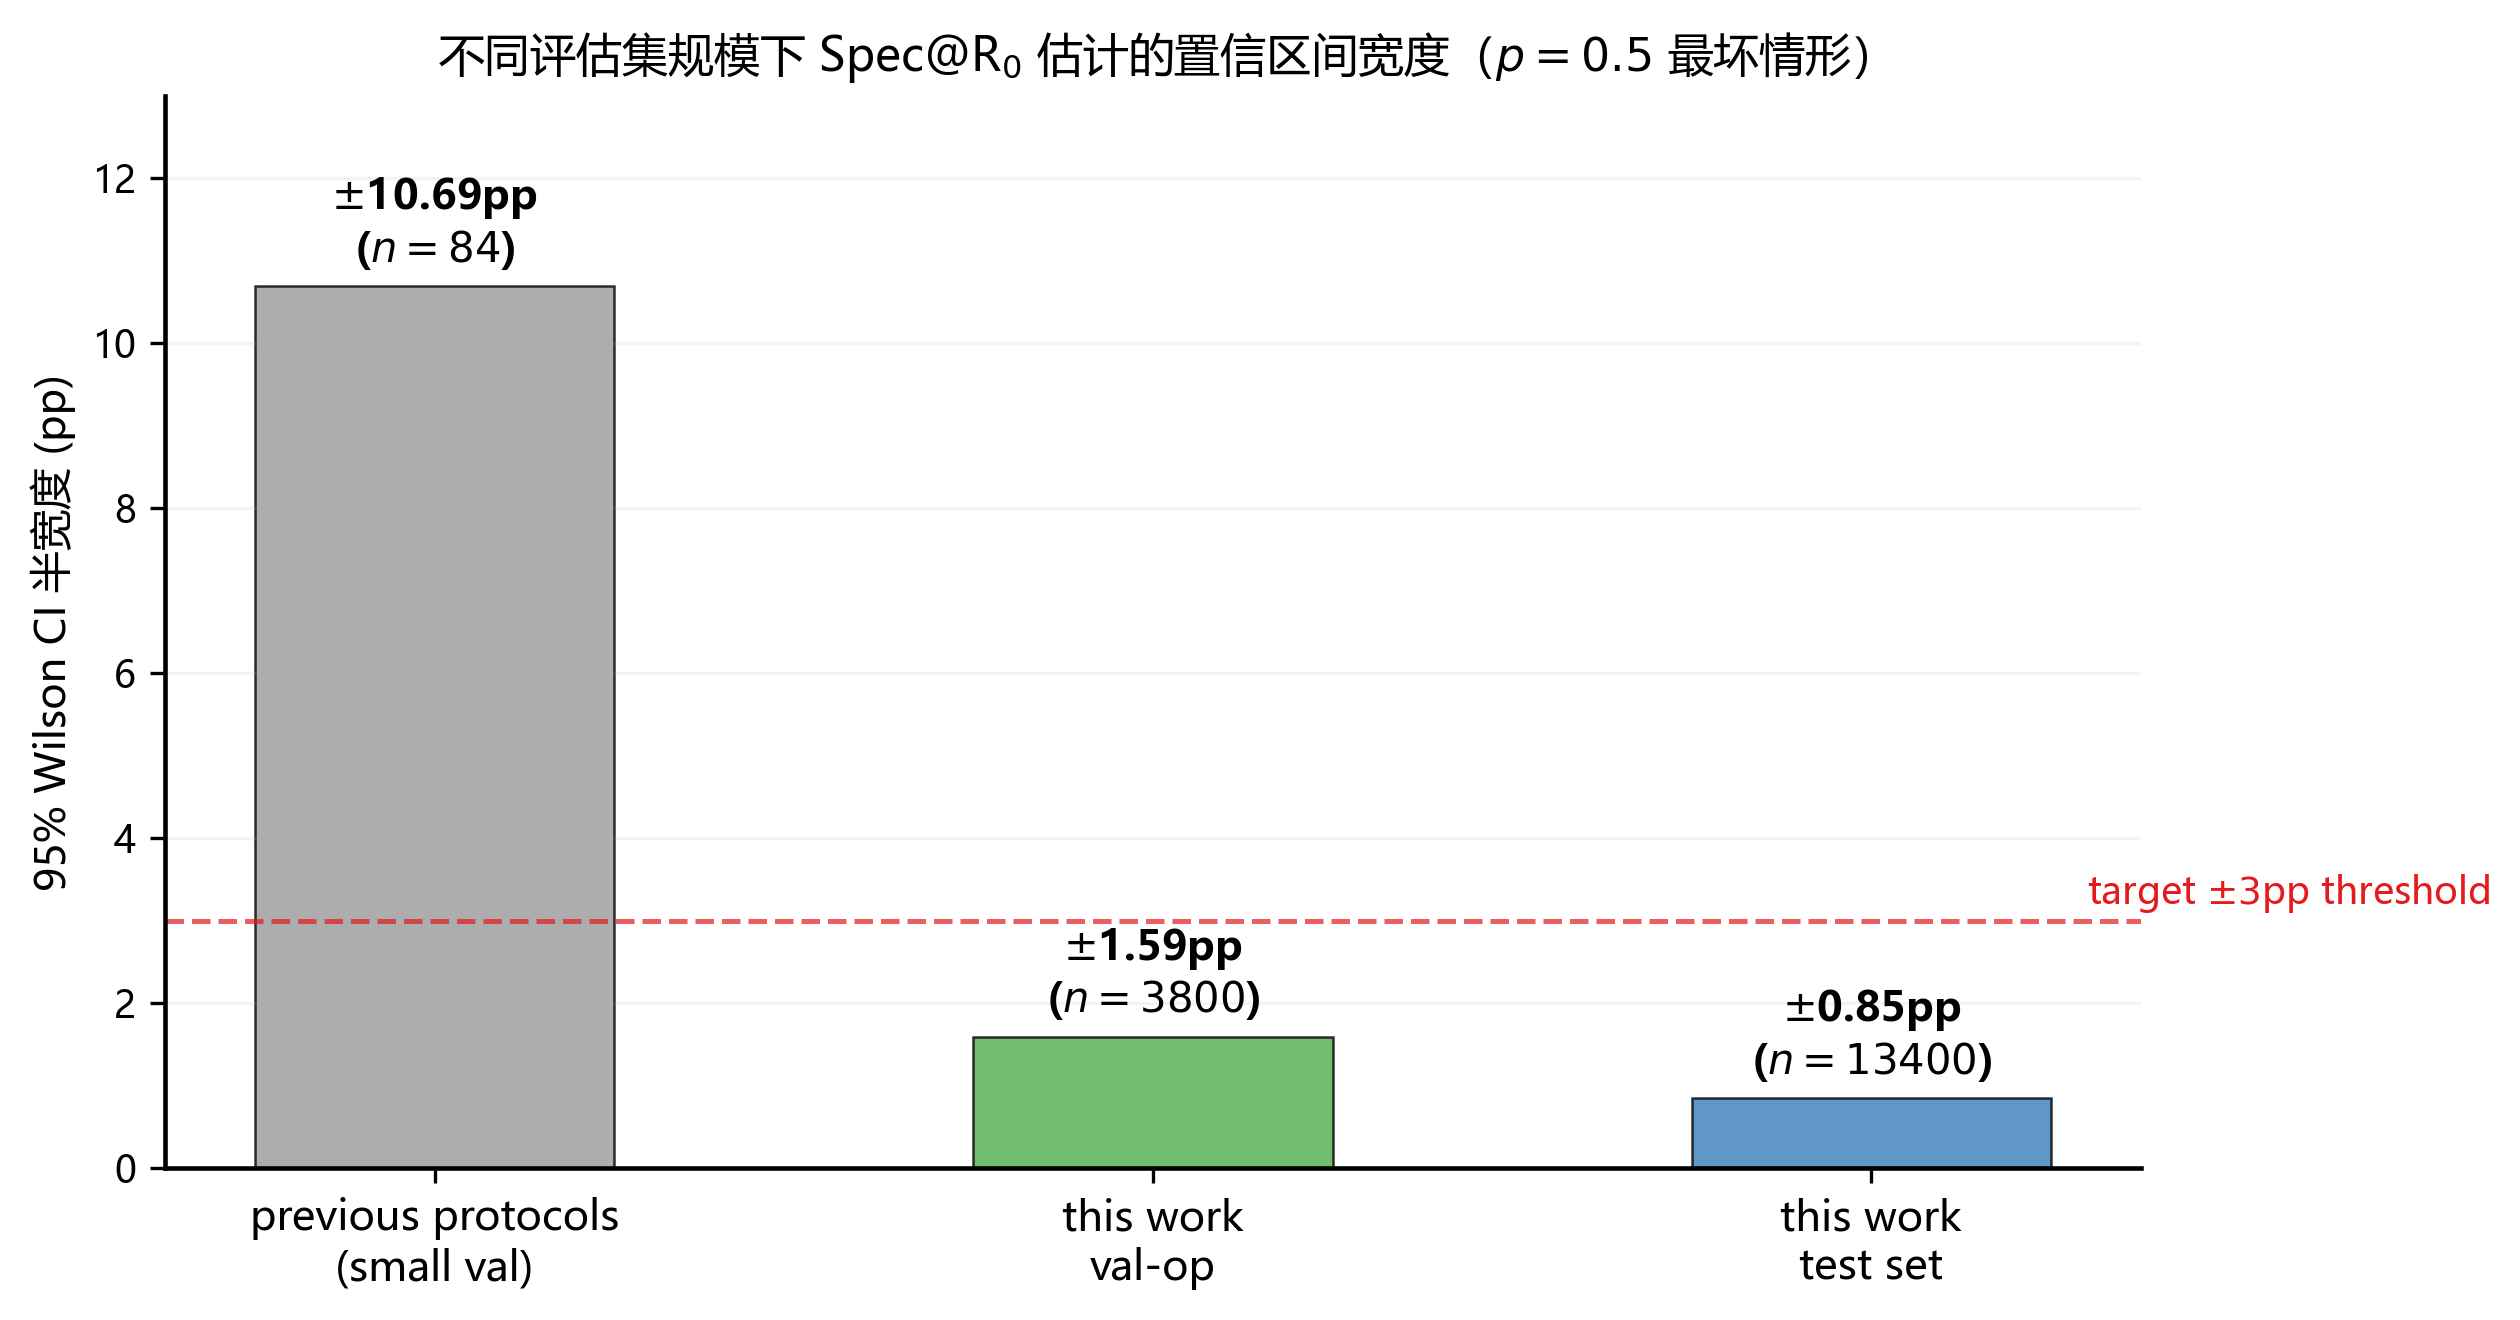
\includegraphics[width=0.88\textwidth]{ch3_ci_comparison.png}
    \caption{\textbf{[Wilson 公式理论计算示意图]} 三种评估集规模下 Spec@R$_0$ 估计的 95\% Wilson 置信区间半宽度对比（$p = 0.5$ 最坏情形）。既往排水管道工作常用的 $n = 84$ 量级评估集使半宽度达 $\pm 10$pp，与模型间差异同量级；本文 val-op（约 3{,}800 正常样本）压缩至 $\pm 1.6$pp，test（约 13{,}400 正常样本）进一步收窄至 $\pm 0.85$pp，显著优于"评估精度优于 $\pm 3$pp"的工程目标。本图数值由式~\eqref{eq:wilson-halfwidth} 在对应 $n$ 下解析计算得出，用于指导评估集规模设计；不是实验结果。}
    \label{fig:ch3-ci}
\end{figure}

\subsection{不重叠原则的工程实现}
为保证 $\mathcal{D}_{\rm train} \cap \mathcal{D}_{\rm val} = \emptyset$、$\mathcal{D}_{\rm train} \cap \mathcal{D}_{\rm test} = \emptyset$、$\mathcal{D}_{\rm val} \cap \mathcal{D}_{\rm test} = \emptyset$，采样过程输出每个子集的完整图像 ID 清单并做去重校验。所有后续脚本通过图像 ID（Sewer-ML 原始文件名）而非路径引用样本，彻底规避因路径变化导致的意外泄漏。

\subsection{帧间相关性与数据源约束下的独立性处理}
\label{sec:pipe-level-independence}
CCTV 排水管道检测数据的一项关键特性是\textbf{帧间强相关}：同一段视频中相邻帧共享相同的管壁材质、光照条件、缺陷实例与摄像机视角。若忽视该相关性任意划分训练/验证/测试集，同一条管道的帧可能被分到不同子集，造成隐式的训练—评估泄漏，并使后续 Wilson 置信区间（式~\eqref{eq:wilson-halfwidth}）的独立同分布假设失真。

本文的数据源存在两项客观约束，使"沿用 Sewer-ML 原生三分划分"的理想做法不可执行：其一，Sewer-ML 的 Val 与 Test 分划图像在本地部署环境中未本地化，短期内无网络下载条件；其二，Sewer-ML Test 的标签由 Codalab leaderboard\cite{haurum2021sewerml} 持有，不对本地评估开放，任何以 SewerML Test 为本文最终评估集的方案都不得不通过 Codalab 在线提交，提交次数受限且不支持本文所需的细粒度指标分解。在此客观条件下，本文将 $\mathcal{D}_{\rm train}$、$\mathcal{D}_{\rm val\text{-}cal}$、$\mathcal{D}_{\rm val\text{-}op}$、$\mathcal{D}_{\rm test}$ 四个子集均抽自 Sewer-ML Train 分划（1{,}040{,}129 张带完整标签的帧）。

该选择带来一项相应的独立性处理约束：Sewer-ML Train 内部的 inspection（管段）粒度 metadata 未在 \texttt{SewerML\_Train.csv} 的任何字段中给出，帧 filename 为 \texttt{00000001.png} 至 \texttt{01300201.png} 的全局顺序编号，不含 inspection\_id 信息。因此，本文\textbf{不声称四子集之间具有 inspection 级独立性}，而采取以下三项可审计的工程处理：
\begin{itemize}[leftmargin=2em,nosep]
\item \textbf{自然稀释}：四子集总规模 $\approx 52{,}000$ 张，占 Sewer-ML Train 分划（$\approx 1.04$M 张）的 5.0\%。即使同 inspection 帧的典型规模为数十至数百张量级，被同时分配到 $\mathcal{D}_{\rm train}$ 与 $\mathcal{D}_{\rm test}$ 的期望发生率亦随整体抽取率线性下降。
\item \textbf{frame-level 随机划分}：以固定种子 \texttt{20260417} 对 Sewer-ML Train 的合格样本池做一次性无重复随机抽样，不引入任何启发式分组或分层，亦不做 per-inspection 帧数上限（后者在无 inspection\_id 时不可实现）。
\item \textbf{残留相关性的显式量化}：\ref{sec:stat-limitations} 节同时给出基于独立同分布假设的 Wilson 半宽度与基于 filename-连续块的 block bootstrap 区间，以量化同 inspection 残留相关性对置信区间宽度的影响。
\end{itemize}

需要指出：上述处理不等价于 inspection 级独立，其关键优势在于\textbf{可执行且诚实}——本文不以"继承 Sewer-ML 的上游管段划分"的名义宣告一条实际未被验证的独立性保证，而是直接将不确定性推到 Wilson 区间与 bootstrap 区间的差距中，供读者与后续工作评估。

\subsection{反向构造样本的训练-only 原则}
\label{sec:train-only-construction}
除划分阶段的独立性外，本文在\textbf{训练侧样本构造}环节设置一条更强的约束：凡是\textbf{会反向影响训练分布}的样本选择动作，其候选池必须\textbf{只来自} $\mathcal{D}_{\rm train}$，不得触及 $\mathcal{D}_{\rm val}$ 或 $\mathcal{D}_{\rm test}$。这类动作在本文涵盖如下：
\begin{itemize}[leftmargin=2em,nosep]
\item Ch5 的困难负样本（Hard Negative）挖掘与 Goldilocks 候选池构造；
\item 基于模型打分的 RDTC 样本价值排序及其导出的训练-子集选择；
\item 类别加权（class weights）、样本重加权（sample reweighting）与课程难度排序；
\item 伪标签（pseudo-label）生成与噪声标签过滤清单；
\item 数据驱动的预处理统计量（均值、标准差、PCA 白化基）估计。
\end{itemize}
该原则的严格性独立于 \ref{sec:pipe-level-independence} 节关于 inspection 级独立性的客观局限：无论底层数据源是否具备 inspection metadata，一旦用 val/test 的任何信息参与上述反向构造，val/test 就从"评估集"退化为"隐式训练信号"，最终的 test 指标不再是独立保留样本上的泛化估计。本文 Ch5 及后续章节的所有样本价值信号 $R, D, T, C$ 的打分输入池均固定为 $\mathcal{D}_{\rm train}$ 的\textbf{正常样本子集}；预处理采用 ImageNet 固定均值与标准差以自动满足此约束。

\section{等条件共享训练协议}
\label{sec:shared-protocol}

为使五种 YOLO11-cls 容量的对比结果可归因于\textbf{容量本身}而非训练超参数的差异，本文在五容量上采用\textbf{完全相同的训练协议}（ceteris paribus），即\textbf{等条件共享训练协议}。表~\ref{tab:shared-protocol} 汇总协议的全部关键超参数。

\begin{table}[H]
    \centering
    \caption{等条件共享训练协议的关键超参数}
    \label{tab:shared-protocol}
    \begin{tabularx}{\textwidth}{p{3.6cm}p{3.2cm}X}
        \toprule
        超参数 & 取值 & 决策依据 \\
        \midrule
        初始权重 & ImageNet 预训练 & 迁移学习\cite{yosinski2014transferable}；见 2.6 节 \\
        输入分辨率 imgsz & 224                & YOLO11-cls 预训练原始分辨率\cite{jocher2023ultralytics} \\
        批大小 batch & 24                     & 四种容量在单 GPU 显存允许的统一上限 \\
        训练轮次 epochs & 200                 & 覆盖从拟合到过拟合的完整轨迹 \\
        优化器 & auto (SGD)                   & Ultralytics 默认，基于 batch 与样本量自动选择 \\
        学习率 & $\mathrm{auto}$              & Ultralytics 基于 batch 自动估计 \\
        早停 patience & 0                     & 禁用早停以保留完整训练轨迹（供 $T$ 信号计算） \\
        save\_period   & 1                    & 每个 epoch 保存检查点 \\
        随机种子 & 0                          & 保证训练可重现 \\
        输入增强 & YOLO 默认                  & 水平翻转、小幅缩放、色彩抖动，与 $C$ 信号的 TTA 扰动独立 \\
        \bottomrule
    \end{tabularx}
\end{table}

协议的两项非默认选择需要特别说明：

\textbf{禁用早停（patience $= 0$）}。常见训练实践会在验证损失若干 epoch 不下降后提前终止以节省计算。本文禁用早停的理由有二：其一，召回约束下的 Spec@R$_0$ 与默认验证损失（通常为交叉熵）存在目标错位（见 1.1 节），按验证损失早停可能错过召回约束下的最优检查点；其二，训练动态信号 $T$ 需要对同一样本在多个训练时间点上的校准概率做方差估计（见式~\eqref{eq:signal-T}），早停会截断训练轨迹，导致 $T$ 信号可用采样点减少。

\textbf{保留每个 epoch 的检查点（save\_period $= 1$）}。本文的评估协议（见 \ref{sec:eval-impl}）在每个 epoch 的检查点上独立运行温度拟合与阈值搜索，选择在 val-op 上 Spec@R$_0$ 最优的 epoch 作为最终模型。该做法相比默认的"仅保存最后一个 epoch"增加了约 200 倍的磁盘开销，但使得 Ch2 讨论的"逐 epoch 召回约束选模"成为可能。

\section{评估协议实施}
\label{sec:eval-impl}

本节将 Ch2 的理论定义转化为可执行的评估流水线。完整流程如图~\ref{fig:ch3-eval-pipeline} 所示，由四个步骤组成。

\subsection{步骤 1：在 val-cal 上拟合温度 $T$}
温度缩放方法最早由 Guo 等\cite{guo2017calibration} 在 ICML 2017 上提出：在 logit 空间除以一个正标量 $T$ 再过 sigmoid，通过最小化独立校准集上的负对数似然（negative log-likelihood, NLL）估计最优 $T^{\ast}$。本文直接采用该方法。

对检查点 $\theta$，记其输出的 logit 为 $z_{\theta}(x)$。在 $\mathcal{D}_{\rm val\text{-}cal}$ 上求解 Guo 等\cite{guo2017calibration} 给出的 NLL 目标：
\begin{equation}
T^{\ast}(\theta) = \arg\min_{T > 0}\; \sum_{(x, y) \in \mathcal{D}_{\rm val\text{-}cal}} \Bigl[-y\log\sigma(z_{\theta}(x)/T) - (1-y)\log(1 - \sigma(z_{\theta}(x)/T))\Bigr].
\label{eq:T-fit-implementation}
\end{equation}
优化采用 L-BFGS 算法，迭代上限 200 次。初始 $T_0 = 1$，实际收敛通常在 30--50 次迭代内完成。得到 $T^{\ast}$ 后，对任意样本 $x$ 的校准概率为 $p_{\rm cal}(x) = \sigma(z_{\theta}(x) / T^{\ast})$。

\subsection{步骤 2：在 val-op 上搜索阈值 $\tau_{R_0}$}
召回约束下的阈值选择遵循 Elkan\cite{elkan2001foundations} 在 IJCAI 2001 上的成本敏感分类理论：对已校准的概率输出，最优决策阈值由应用层成本/约束决定，可在校准集上通过重新搜索得到而无需改动训练。本文以固定召回下界 $R_0$ 替代显式错分代价，定义召回约束最优阈值为满足约束的最小阈值：
\begin{equation}
\tau_{R_0}(\theta) = \min\bigl\{\tau \in [0, 1] : \mathrm{Recall}_{\mathcal{D}_{\rm val\text{-}op}}(\tau) \geq R_0\bigr\}.
\label{eq:tau-search}
\end{equation}

实际计算步骤：将 $\mathcal{D}_{\rm val\text{-}op}$ 中所有异常样本（$y = 1$）的校准概率集合 $\{p_{\rm cal}(x)\}_{x \in \mathcal{A}}$ 降序排序，取第 $\lceil R_0 \cdot |\mathcal{A}| \rceil$ 大的分数作为 $\tau_{R_0}$。本文分别对 $R_0 \in \{0.995, 0.990\}$ 求解 $\tau_{99.5}$ 与 $\tau_{99.0}$。在同一组校准概率上计算\textbf{经典二分类混淆矩阵指标}（参见 Provost 与 Fawcett\cite{provost2001robust}）的四项：
\begin{align}
\mathrm{Spec@R}_0 &= \frac{|\{x \in \mathcal{N} : p_{\rm cal}(x) < \tau_{R_0}\}|}{|\mathcal{N}|}, \label{eq:spec-implement}\\
\mathrm{Prec@R}_0 &= \frac{|\{x \in \mathcal{A} : p_{\rm cal}(x) \geq \tau_{R_0}\}|}{|\{x \in \mathcal{N} \cup \mathcal{A} : p_{\rm cal}(x) \geq \tau_{R_0}\}|}, \label{eq:prec-implement}\\
\mathrm{PTR@R}_0 &= \frac{|\{x \in \mathcal{D}_{\rm val\text{-}op} : p_{\rm cal}(x) \geq \tau_{R_0}\}|}{|\mathcal{D}_{\rm val\text{-}op}|}, \label{eq:ptr-implement}
\end{align}
其中 $\mathcal{N}, \mathcal{A}$ 分别为正常、异常样本集合，PTR 为通过率（pass-through rate，进入下一阶段的样本占比）。由此同时得到 $\mathrm{Spec@R99.5}$、$\mathrm{Spec@R99.0}$、$\mathrm{Prec@R99.0}$、$\mathrm{PTR@R99.0}$ 四项指标。

\subsection{步骤 3：按四元字典序选最优 epoch}
字典序（lexicographic order）是多目标决策中的经典排序规则，在 Settles\cite{settles2009active} 的主动学习综述等多准则评价文献中被广泛使用：按优先级依次比较指标，前序指标打平时才由后序指标裁决。本文将其专用化为\textbf{门控任务的四元字典序}，构造基于召回约束下四项指标的综合排序函数
\begin{equation}
\mathrm{rank}(\theta) = \mathrm{lex}\bigl(\mathrm{Spec@R99.5}(\theta),\; \mathrm{Spec@R99.0}(\theta),\; \mathrm{Prec@R99.0}(\theta),\; -\mathrm{PTR@R99.0}(\theta)\bigr),
\label{eq:lex-rank-implement}
\end{equation}
前三项为越大越优，末项 PTR 越小越优（通过率低意味着更少的人工复核）故取负号。该字典序的优先级选择反映本文对门控任务的工程偏好：首先要保证最严格召回下的拦截率（Spec@R99.5），其次看略放松召回下的拦截率（Spec@R99.0），再次看精度（Prec@R99.0），最后用 PTR 作为在前三项打平时的最终断点。具体实施时，对同一训练 run 的 200 个检查点 $\{\theta_1, \theta_2, \ldots, \theta_{200}\}$ 按式~\eqref{eq:lex-rank-implement} 排序，选取排第一的 epoch 作为该 run 的\textbf{最优检查点} $\theta^{\ast}$。最优检查点对应的四项指标即为该 run 的最终报告值。

\subsection{步骤 4：在测试集上一次性重评}
步骤 1--3 基于验证集完成。选出 $\theta^{\ast}$ 后，将其 $T^{\ast}(\theta^{\ast})$ 与 $\tau_{99.5}(\theta^{\ast}), \tau_{99.0}(\theta^{\ast})$ 冻结，应用到测试集 $\mathcal{D}_{\rm test}$ 上\textbf{仅推理一次}，报告测试集 Spec@R99.5 与 Spec@R99.0。测试集推理\textbf{不重新拟合 $T$、不重新搜索 $\tau$}，以确保测试指标完全独立于任何验证集上的决策。

\begin{figure}[H]
    \centering
    \begin{tikzpicture}[
        node distance=0.75cm,
        box/.style={draw, rounded corners=3pt, minimum width=3.8cm, minimum height=0.9cm, align=center, font=\small},
        arr/.style={-{Stealth[length=2mm,width=2mm]}, thick}
    ]
    \node[box, fill=blue!8] (ckpt) {训练得到 200 个 epoch \\ 检查点 $\{\theta_t\}_{t=1}^{200}$};
    \node[box, fill=green!10, right=1.6cm of ckpt] (s1) {Step 1: 在 val-cal 上 \\ 拟合 $T^{\ast}(\theta_t)$};
    \node[box, fill=green!10, below=of s1] (s2) {Step 2: 在 val-op 上 \\ 搜索 $\tau_{99.5}, \tau_{99.0}$};
    \node[box, fill=green!10, below=of s2] (s3) {Step 3: 按四元字典序 \\ 选 $\theta^{\ast}$};
    \node[box, fill=orange!15, below=of s3] (s4) {Step 4: 在 test 上 \\ 冻结 $(T^{\ast}, \tau^{\ast})$ 评估};
    \node[box, fill=red!10, left=1.6cm of s3] (out) {最终指标： \\ Spec@R99.5, Spec@R99.0};
    \draw[arr] (ckpt) -- (s1);
    \draw[arr] (s1) -- (s2);
    \draw[arr] (s2) -- (s3);
    \draw[arr] (s3) -- (s4);
    \draw[arr] (s4) -| (out);
    \end{tikzpicture}
    \caption{评估协议实施流程。前三步在验证集上完成（用于选模与调阈），第四步在测试集上冻结参数一次性评估。}
    \label{fig:ch3-eval-pipeline}
\end{figure}

\subsection{统计推断的局限与处理}
\label{sec:stat-limitations}
前四步给出的指标点估计与置信区间依赖两项假设，本节显式说明本文对这两项假设的处理方式及其保守性定位。

\textbf{一、帧间相关使 Wilson 区间为乐观下界}。式~\eqref{eq:wilson-halfwidth} 的 Wilson 半宽度公式\cite{wilson1927probable} 基于独立同分布 Bernoulli 假设推导；如 \ref{sec:pipe-level-independence} 节所述，本文四子集共源于 Sewer-ML Train，且 inspection\_id 不可得，因此\textbf{同 inspection 的相邻帧跨子集分布}的残留相关性无法完全排除，使测试集的有效独立样本数 $n_{\rm eff} < n$，实际 95\% 覆盖半宽度\textbf{大于}式~\eqref{eq:wilson-halfwidth} 算出的数值。本文对该局限采取两项处理：其一，正文中的 Wilson 半宽度均明确标注为\textbf{独立性假设下的下界估计}，不作为最终紧上界呈现；其二，在 \ref{sec:pipe-level-independence} 节的 frame-level 随机划分无法做 inspection 级 bootstrap 的条件下，本文改用\textbf{filename 连续块 bootstrap}\cite{kunsch1989jackknife} 作为 inspection-level bootstrap 的工程代理：将 $\mathcal{D}_{\rm test}$ 按 filename 排序后每连续 50 张构成一个块（Sewer-ML 的 filename 全局顺序编号在大概率上对 inspection 内帧是保序的，相邻 filename 倾向于来自同一段 CCTV 视频），按块放回重采样 $B = 2000$ 次，每次在采得的块集合上重新计算 Spec@R$_0$，取 $B$ 次估计的 2.5\% 与 97.5\% 分位数作为稳健区间，与 Wilson 区间并列汇报。块大小 50 的选择兼顾了"大于典型 inspection 帧数的十分之一"与"小于测试集总体的百分之一"两项经验约束。

\textbf{二、阈值在 val-op 上通过"选择"获得，val-op 上的指标为乐观估计}。式~\eqref{eq:tau-search} 定义的 $\tau_{R_0}(\theta)$ 是在 $\mathcal{D}_{\rm val\text{-}op}$ 上扫描所有候选阈值后"选出"的最小满足召回约束的阈值，此选择过程使 $\mathcal{D}_{\rm val\text{-}op}$ 上评得的 $\mathrm{Spec@R_0}$ 系统性偏高——这是"在同一集上既定阈值又报告指标"的典型选择偏差，Platt\cite{platt1999probabilistic} 与 Guo 等\cite{guo2017calibration} 均在各自的校准方法论中强调需用独立集汇报最终指标。本文严格区分两套数字：$\mathcal{D}_{\rm val\text{-}op}$ 上的指标仅在"选模与调阈"的过程语境下出现，用于按字典序（式~\eqref{eq:lex-rank-implement}）选 $\theta^{\ast}$；\textbf{主结果一律汇报测试集数字}——$\tau_{R_0}(\theta^{\ast})$ 冻结后在独立的 $\mathcal{D}_{\rm test}$ 上重评，测试指标完全独立于任何阈值选择决策。论文正文在"主要结果"部分默认引用测试集数字；验证集数字仅在"选模过程说明"的语境下附录式出现，避免读者将两者混淆。

\textbf{三、协议冻结（protocol freeze）以防止 val-op 退化为元训练集}。上述第二项只约束了\textbf{阈值选择}本身不污染 val-op，但还存在一个更隐蔽的渠道：若研究者在观察 val-op 上的阶段性指标后，反复修改类映射、OK/PH 过滤规则、采样规则、增强策略或字典序规则，则 val-op 在事实上被用作\textbf{元训练集}（meta-training set）——test 虽未被触及，但被 val-op "对齐"过的模型在 test 上的数字依然承载了 val-op 的选择偏差。Ng\cite{ng2017machine} 在机器学习工程实践中称此现象为"验证集过拟合"（validation overfitting）。本文采取的处理是\textbf{协议冻结}：在正式大规模训练开始前，将 \ref{sec:sampling} 节的采样规则、\ref{sec:split-sizes} 节的划分规模、\ref{sec:shared-protocol} 节的训练超参、\ref{sec:eval-impl} 节前四步的评估流程与字典序规则全部定稿，形成 \texttt{sampling\_protocol\_v1.yaml} 与 \texttt{training\_protocol\_v1.yaml} 两份版本化配置；冻结之后，任何基于 val-op 结果的规则修改都须发版至 \texttt{v2} 并触发三子集的\textbf{完整重抽}，论文正文同时汇报新旧两版结果以保持可审计。该流程确保 val-op 的角色始终限定为"用于按固定字典序选 $\theta^{\ast}$ 的决定函数输入"，而非"开发期反复咨询的设计参考"。

\subsection{四信号的计算实施}
\label{sec:rdtc-compute}
RDTC 四信号的计算\textbf{集中在最优检查点} $\theta^{\ast}$ 上进行，而非在每个 epoch 上对每个样本重复计算。这样做的理由有二：其一，选优后的 $\theta^{\ast}$ 是模型在召回约束下的最佳状态，对样本价值的打分最贴近部署意义；其二，多信号逐 epoch 计算需要数百倍于单检查点的推理量，计算成本不可控。四个信号的具体实施步骤如下（为避免读者回翻 Ch2，计算式在此直接展开）。

\textbf{$R(x)$——边界风险}。边界风险的思想源自 Lewis 与 Gale\cite{lewis1994sequential} 在 SIGIR 1994 上提出的不确定性采样原则——靠近决策边界的样本对模型训练信息量最大；Settles\cite{settles2009active} 的综述将该原则系统化为多个变体，二分类下 margin-based 形式与"到 0.5 的距离的倒数"等价。本文按 Lewis 与 Gale 的不确定性采样思路，在温度校准后的概率空间上具体化为：
\begin{enumerate}[leftmargin=2em,nosep]
\item 对候选样本 $x$ 做一次前向传播，得到 $\theta^{\ast}$ 输出的 logit $z^{\ast}(x) \in \mathbb{R}$；
\item 用已拟合的温度 $T^{\ast}$ 做校准，得到校准概率 $p^{\ast}(x) = \sigma(z^{\ast}(x) / T^{\ast}) = 1/(1 + e^{-z^{\ast}(x)/T^{\ast}})$；
\item 按样本到决策边界 $p = 0.5$ 的距离的倒数打分：
\begin{equation}
R(x) = \frac{1}{\bigl|\,p^{\ast}(x) - 0.5\,\bigr| + \epsilon}, \quad \epsilon = 10^{-6}.
\label{eq:R-implement}
\end{equation}
$R(x)$ 越大，样本在校准概率空间上越靠近决策边界。
\end{enumerate}
计算成本：每样本 1 次前向传播。候选池规模 $N_{\rm pool}$ 下总成本 $O(N_{\rm pool})$。

\textbf{$D(x)$——邻域密度}。邻域密度对应 Sener 与 Savarese\cite{sener2018active} 在 ICLR 2018 上提出的核心集选样框架：样本价值应由其在特征空间中的几何代表性刻画，通过与 $k$ 近邻的相似度均值衡量样本所在区域的稠密程度。本文按该几何视角，使用骨干倒数第二层特征与 $k$ 近邻余弦相似度均值作为 $D$ 信号：
\begin{enumerate}[leftmargin=2em,nosep]
\item 对 $\theta^{\ast}$ 移除最后的分类层，保留\textbf{全局平均池化后的特征向量} $\phi(x) \in \mathbb{R}^{d}$（$d$ 由骨干容量决定，本文五容量的 $d$ 均为 1280）；
\item 对每个候选样本做一次前向传播并提取 $\phi(x)$，得到候选池的特征矩阵 $\Phi \in \mathbb{R}^{N_{\rm pool} \times d}$；
\item $L_2$ 归一化每行：$\tilde{\phi}(x) = \phi(x) / \|\phi(x)\|_2$；
\item 对每个样本 $x$，计算 $\tilde{\phi}(x)$ 与候选池其他所有样本的余弦相似度，取其中最大的 $k$ 个（排除自身，本文 $k = 25$），得 $k$ 近邻集合 $\mathrm{kNN}(x)$；
\item 该 $k$ 个相似度的算术平均作为密度打分：
\begin{equation}
D(x) = \frac{1}{k}\sum_{y \in \mathrm{kNN}(x)} \tilde{\phi}(x)^{\top}\tilde{\phi}(y).
\label{eq:D-implement}
\end{equation}
\end{enumerate}
$D(x)$ 越大（越接近 1），样本越位于特征空间的稠密聚类区；越小（趋于 0），样本越孤立。计算成本：前向传播 $O(N_{\rm pool})$ + kNN 搜索 $O(N_{\rm pool}^2 d)$（或用 FAISS 近似检索降至 $O(N_{\rm pool} \log N_{\rm pool})$）。

\textbf{$T(x)$——训练动态}。训练动态信号的核心思想由 Toneva 等\cite{toneva2019empirical} 在 ICLR 2019 上以"遗忘事件"概念首次引入，随后 Swayamdipta 等\cite{swayamdipta2020cartography} 在 EMNLP 2020 上将其细化为\textbf{数据集制图}框架，按跨 epoch 置信度均值与标准差将样本映射到模糊/易学/难学三区域，并证明\emph{标准差越大的样本（模糊样本）对训练贡献越大}。本文以 Swayamdipta 等定义的跨 epoch 置信度标准差作为 $T$ 信号，具体实施如下：
\begin{enumerate}[leftmargin=2em,nosep]
\item 从训练保留的 200 个 epoch 检查点中，选取\textbf{训练中后段}的 $L$ 个时间点 $\mathcal{T} = \{t_1, t_2, \ldots, t_L\}$（本文取 $\mathcal{T} = \{120, 140, 160, 180, 200\}$，即训练末期每 20 epoch 取一点）；
\item 在每个 $t \in \mathcal{T}$ 对应的检查点 $\theta_t$ 上：
  \begin{enumerate}[leftmargin=2em,nosep]
  \item[(a)] 在当前检查点的 val-cal 上重新拟合温度 $T_t^{\ast}$；
  \item[(b)] 对候选样本 $x$ 前向传播得 $z_t(x)$；
  \item[(c)] 校准得 $p_t(x) = \sigma(z_t(x)/T_t^{\ast})$；
  \end{enumerate}
\item 收集时间序列 $\{p_t(x)\}_{t \in \mathcal{T}}$，按 Swayamdipta 等\cite{swayamdipta2020cartography} 的定义计算其样本标准差：
\begin{equation}
\bar{p}(x) = \frac{1}{L}\sum_{t \in \mathcal{T}} p_t(x), \qquad
T(x) = \sqrt{\frac{1}{L}\sum_{t \in \mathcal{T}}\bigl(p_t(x) - \bar{p}(x)\bigr)^2}.
\label{eq:T-implement}
\end{equation}
\end{enumerate}
$T(x)$ 越大，样本在训练后段预测波动越剧烈，对应 Swayamdipta 等\cite{swayamdipta2020cartography} 所识别的"模糊"样本。计算成本：每样本 $L$ 次前向传播，总 $O(L \cdot N_{\rm pool})$。

\textbf{$C(x)$——扰动一致性}。扰动一致性源自 Gal 等\cite{gal2017deep} 在 ICML 2017 上提出的深度贝叶斯主动学习：对同一输入做多次随机扰动推理，预测方差即为样本不确定性；Beluch 等\cite{beluch2018power} 在 CVPR 2018 上用模型集成替代 Dropout 扰动得到类似结论。本文将扰动源迁移至输入侧（测试时增强），沿用二者的"扰动下预测方差 = 样本不确定性"核心思想，按下列步骤计算：
\begin{enumerate}[leftmargin=2em,nosep]
\item 选定一组保持语义的输入扰动 $\mathcal{A} = \{a_1, a_2, \ldots, a_{|\mathcal{A}|}\}$。本文 $\mathcal{A}$ 包含 6 种扰动：恒等（原图）、水平翻转、$\pm 10^{\circ}$ 小角度旋转、随机裁剪至 $0.9\times$ 再上采样、亮度 $\pm 20\%$ 抖动、轻度高斯模糊（$\sigma = 0.5$）；
\item 对每个候选样本 $x$ 与每种扰动 $a_i$，做前向传播得 $z_i(x) = z_{\theta^{\ast}}(a_i(x))$；
\item 校准得 $p_i(x) = \sigma(z_i(x)/T^{\ast})$，收集 $\{p_i(x)\}_{i=1}^{|\mathcal{A}|}$；
\item 按 Gal 等\cite{gal2017deep} 所用的"扰动方差"形式（本文取 1 减方差的归一化形式使数值介于 0--1 且越大越稳）打分：
\begin{equation}
C(x) = 1 - \frac{1}{|\mathcal{A}|}\sum_{i=1}^{|\mathcal{A}|}\bigl(p_i(x) - \bar{p}_{\mathcal{A}}(x)\bigr)^2, \quad
\bar{p}_{\mathcal{A}}(x) = \frac{1}{|\mathcal{A}|}\sum_{i=1}^{|\mathcal{A}|} p_i(x).
\label{eq:C-implement}
\end{equation}
\end{enumerate}
$C(x)$ 越接近 1，样本在扰动下预测越稳定；越小表示扰动轻微即改变判断，对应边界附近或特征不稳定的样本。计算成本：每样本 $|\mathcal{A}|$ 次前向传播，总 $O(|\mathcal{A}| \cdot N_{\rm pool})$。

\textbf{四信号整合与候选池规模}。四个信号对候选池中的每个样本分别输出一个实数分数，构成四元特征向量 $(R(x), D(x), T(x), C(x))$。在后续第 6 章的分位数分层消融实验中，将候选样本按任一单信号升/降序排序，均分为 $Q$ 个分位桶进行消融比较。本文候选池 $N_{\rm pool}$ 规模由第 5 章实验章节确定，典型取 $10^3$--$10^4$ 量级——该规模既保证每个分位桶内样本数足以训练出有区分度的模型，又使四信号计算的总推理量在计算预算之内。

\backmatter
\begin{thebibliography}{99}

\bibitem{lecun1998gradient}
LeCun Y, Bottou L, Bengio Y, Haffner P. Gradient-Based Learning Applied to Document Recognition[J]. Proceedings of the IEEE, 1998, 86(11): 2278--2324.

\bibitem{krizhevsky2012imagenet}
Krizhevsky A, Sutskever I, Hinton G E. ImageNet Classification with Deep Convolutional Neural Networks[C]//Advances in Neural Information Processing Systems. 2012: 1097--1105.

\bibitem{simonyan2015vgg}
Simonyan K, Zisserman A. Very Deep Convolutional Networks for Large-Scale Image Recognition[C]//International Conference on Learning Representations. 2015.

\bibitem{he2016resnet}
He K, Zhang X, Ren S, Sun J. Deep Residual Learning for Image Recognition[C]//Proceedings of the IEEE Conference on Computer Vision and Pattern Recognition. 2016: 770--778.

\bibitem{nair2010relu}
Nair V, Hinton G E. Rectified Linear Units Improve Restricted Boltzmann Machines[C]//Proceedings of the 27th International Conference on Machine Learning. 2010: 807--814.

\bibitem{ioffe2015batchnorm}
Ioffe S, Szegedy C. Batch Normalization: Accelerating Deep Network Training by Reducing Internal Covariate Shift[C]//Proceedings of the 32nd International Conference on Machine Learning. 2015: 448--456.

\bibitem{redmon2017yolov2}
Redmon J, Farhadi A. YOLO9000: Better, Faster, Stronger[C]//Proceedings of the IEEE Conference on Computer Vision and Pattern Recognition. 2017: 6517--6525.

\bibitem{redmon2018yolov3}
Redmon J, Farhadi A. YOLOv3: An Incremental Improvement[J]. arXiv preprint arXiv:1804.02767, 2018.

\bibitem{bochkovskiy2020yolov4}
Bochkovskiy A, Wang C Y, Liao H Y M. YOLOv4: Optimal Speed and Accuracy of Object Detection[J]. arXiv preprint arXiv:2004.10934, 2020.

\bibitem{platt1999probabilistic}
Platt J C. Probabilistic Outputs for Support Vector Machines and Comparisons to Regularized Likelihood Methods[C]//Advances in Large Margin Classifiers. MIT Press, 1999: 61--74.

\bibitem{moradi2019review}
Moradi S, Zayed T, Golkhoo F. Review on Computer Aided Sewer Pipeline Defect Detection and Condition Assessment[J]. Infrastructures, 2019, 4(1): 10.

\bibitem{haurum2020survey}
Haurum J B, Moeslund T B. A Survey on Image-Based Automation of CCTV and SSET Sewer Inspections[J]. Automation in Construction, 2020, 111: 103061.

\bibitem{ma2026stateoftheart}
Ma D, Fang H, Wang N, et al. The State-of-the-Art in Pipe Defect Inspection with Computer Vision-Based Methods[J]. Measurement, 2026, 257: 118431.

\bibitem{cjj181}
中华人民共和国住房和城乡建设部. 城镇排水管道检测与评估技术规程: CJJ 181-2012[S]. 北京: 中国建筑工业出版社, 2012.

\bibitem{cheng2018deep}
Cheng J C P, Wang M. Automated Detection of Sewer Pipe Defects in CCTV Images Using Deep Learning Techniques[J]. Automation in Construction, 2018, 95: 155--171.

\bibitem{halfawy2014hogsvm}
Halfawy M R, Hengmeechai J. Automated Defect Detection in Sewer Closed Circuit Television Images Using Histograms of Oriented Gradients and Support Vector Machine[J]. Automation in Construction, 2014, 38: 1--13.

\bibitem{kumar2018cnn}
Kumar S S, Abraham D M, Jahanshahi M R, et al. Automated Defect Classification in Sewer Closed Circuit Television Inspections Using Deep Convolutional Neural Networks[J]. Automation in Construction, 2018, 91: 273--283.

\bibitem{haurum2021sewerml}
Haurum J B, Moeslund T B. Sewer-ML: A Multi-Label Sewer Defect Classification Dataset and Benchmark[C]//Proceedings of the IEEE/CVF Conference on Computer Vision and Pattern Recognition. 2021: 13456--13467.

\bibitem{redmon2016yolo}
Redmon J, Divvala S, Girshick R, Farhadi A. You Only Look Once: Unified, Real-Time Object Detection[C]//Proceedings of the IEEE Conference on Computer Vision and Pattern Recognition. 2016: 779--788.

\bibitem{jocher2023ultralytics}
Jocher G, Chaurasia A, Qiu J. Ultralytics YOLO[EB/OL]. https://github.com/ultralytics/ultralytics, 2023.

\bibitem{wang2023improvedyolov5}
Wang T, Li Y, Zhai Y, et al. A Sewer Pipeline Defect Detection Method Based on Improved YOLOv5[J]. Processes, 2023, 11(8): 2508.

\bibitem{zhao2024yolov5sewer}
Zhao X, Xiao N, Cai Z, et al. YOLOv5-Sewer: Lightweight Sewer Defect Detection Model[J]. Applied Sciences, 2024, 14(5): 1869.

\bibitem{situ2023transfer}
Situ Z, Teng S, Feng W, et al. A Transfer Learning-Based YOLO Network for Sewer Defect Detection in Comparison to Classic Object Detection Methods[J]. Developments in the Built Environment, 2023, 15: 100191.

\bibitem{xie2019hierarchical}
Xie Q, Li D, Xu J, Yu Z, Wang J. Automatic Detection and Classification of Sewer Defects via Hierarchical Deep Learning[J]. IEEE Transactions on Automation Science and Engineering, 2019, 16(4): 1836--1847.

\bibitem{chen2018intelligent}
Chen K, Hu H, Chen C, Chen L, He C. An Intelligent Sewer Defect Detection Method Based on Convolutional Neural Network[C]//IEEE International Conference on Information and Automation. 2018: 1301--1306.

\bibitem{shamsolmoali2025twostage}
Shamsolmoali P, Sadka A H, Savvas I K, et al. Automated Defect Classification and Localization in Sewer Pipelines Using Hybrid ResNet50--Swin Transformer and Modified YOLOv8[J]. Scientific Reports, 2025, 15: 6143.

\bibitem{meijer2019defect}
Meijer D, Scholten L, Clemens F, Knobbe A. A Defect Classification Methodology for Sewer Image Sets with Convolutional Neural Networks[J]. Automation in Construction, 2019, 104: 281--298.

\bibitem{myrans2019automated}
Myrans J, Everson R, Maybury R. Automated Detection of Faults in Sewers Using CCTV Image Sequences[J]. Automation in Construction, 2019, 95: 64--71.

\bibitem{guo2017calibration}
Guo C, Pleiss G, Sun Y, Weinberger K Q. On Calibration of Modern Neural Networks[C]//Proceedings of the 34th International Conference on Machine Learning. 2017: 1321--1330.

\bibitem{minderer2021calibration}
Minderer M, Djolonga J, Romijnders R, et al. Revisiting the Calibration of Modern Neural Networks[C]//Advances in Neural Information Processing Systems. 2021: 15682--15694.

\bibitem{elkan2001foundations}
Elkan C. The Foundations of Cost-Sensitive Learning[C]//Proceedings of the 17th International Joint Conference on Artificial Intelligence. 2001: 973--978.

\bibitem{provost2001robust}
Provost F, Fawcett T. Robust Classification for Imprecise Environments[J]. Machine Learning, 2001, 42(3): 203--231.

\bibitem{kumar2021constrained}
Kumar A, Narasimhan H, Cotter A, Gupta M. Optimizing Specificity at a High Sensitivity[C]//Proceedings of the 38th International Conference on Machine Learning. 2021: 11415--11424.

\bibitem{menon2021longtail}
Menon A K, Jayasumana S, Rawat A S, et al. Long-Tail Learning via Logit Adjustment[C]//International Conference on Learning Representations. 2021.

\bibitem{wilson1927probable}
Wilson E B. Probable Inference, the Law of Succession, and Statistical Inference[J]. Journal of the American Statistical Association, 1927, 22(158): 209--212.

\bibitem{kunsch1989jackknife}
K\"unsch H R. The Jackknife and the Bootstrap for General Stationary Observations[J]. The Annals of Statistics, 1989, 17(3): 1217--1241.

\bibitem{ng2017machine}
Ng A. Machine Learning Yearning: Technical Strategy for AI Engineers in the Era of Deep Learning[M]. Self-published draft, deeplearning.ai, 2018.

\bibitem{clopper1934use}
Clopper C J, Pearson E S. The Use of Confidence or Fiducial Limits Illustrated in the Case of the Binomial[J]. Biometrika, 1934, 26(4): 404--413.

\bibitem{agresti1998approximate}
Agresti A, Coull B A. Approximate is Better than ``Exact'' for Interval Estimation of Binomial Proportions[J]. The American Statistician, 1998, 52(2): 119--126.

\bibitem{lewis1994sequential}
Lewis D D, Gale W A. A Sequential Algorithm for Training Text Classifiers[C]//Proceedings of the 17th Annual International ACM SIGIR Conference on Research and Development in Information Retrieval. 1994: 3--12.

\bibitem{settles2009active}
Settles B. Active Learning Literature Survey[R]. University of Wisconsin--Madison Department of Computer Sciences, Technical Report 1648, 2009.

\bibitem{schein2007active}
Schein A I, Ungar L H. Active Learning for Logistic Regression: An Evaluation[J]. Machine Learning, 2007, 68(3): 235--265.

\bibitem{coleman2020selection}
Coleman C, Yeh C, Mussmann S, et al. Selection via Proxy: Efficient Data Selection for Deep Learning[C]//International Conference on Learning Representations. 2020.

\bibitem{nguyen2004active}
Nguyen H T, Smeulders A. Active Learning Using Pre-clustering[C]//Proceedings of the 21st International Conference on Machine Learning. 2004: 79.

\bibitem{sener2018active}
Sener O, Savarese S. Active Learning for Convolutional Neural Networks: A Core-Set Approach[C]//International Conference on Learning Representations. 2018.

\bibitem{toneva2019empirical}
Toneva M, Sordoni A, des Combes R T, et al. An Empirical Study of Example Forgetting During Deep Neural Network Learning[C]//International Conference on Learning Representations. 2019.

\bibitem{swayamdipta2020cartography}
Swayamdipta S, Schwartz R, Lourie N, et al. Dataset Cartography: Mapping and Diagnosing Datasets with Training Dynamics[C]//Proceedings of the 2020 Conference on Empirical Methods in Natural Language Processing. 2020: 9275--9293.

\bibitem{paul2021deep}
Paul M, Ganguli S, Dziugaite G K. Deep Learning on a Data Diet: Finding Important Examples Early in Training[C]//Advances in Neural Information Processing Systems. 2021: 20596--20607.

\bibitem{gal2017deep}
Gal Y, Islam R, Ghahramani Z. Deep Bayesian Active Learning with Image Data[C]//Proceedings of the 34th International Conference on Machine Learning. 2017: 1183--1192.

\bibitem{beluch2018power}
Beluch W H, Genewein T, Nürnberger A, Köhler J M. The Power of Ensembles for Active Learning in Image Classification[C]//Proceedings of the IEEE Conference on Computer Vision and Pattern Recognition. 2018: 9368--9377.

\bibitem{mindermer2022prioritized}
Mindermann S, Brauner J M, Razzak M T, et al. Prioritized Training on Points that are Learnable, Worth Learning, and Not Yet Learnt[C]//Proceedings of the 39th International Conference on Machine Learning. 2022: 15630--15649.

\bibitem{nassco2020pacp}
National Association of Sewer Service Companies. Pipeline Assessment Certification Program (PACP) Reference Manual, 7th Edition[M]. NASSCO, 2020.

\bibitem{wsa2020}
Water Services Association of Australia. WSA 05-2020 Conduit Inspection Reporting Code of Australia[S]. WSAA, 2020.

\bibitem{pan2010transfer}
Pan S J, Yang Q. A Survey on Transfer Learning[J]. IEEE Transactions on Knowledge and Data Engineering, 2010, 22(10): 1345--1359.

\bibitem{hestness2017scaling}
Hestness J, Narang S, Ardalani N, et al. Deep Learning Scaling is Predictable, Empirically[J]. arXiv preprint arXiv:1712.00409, 2017.

\bibitem{sun2017revisiting}
Sun C, Shrivastava A, Singh S, Gupta A. Revisiting Unreasonable Effectiveness of Data in Deep Learning Era[C]//Proceedings of the IEEE International Conference on Computer Vision. 2017: 843--852.

\bibitem{kornblith2019better}
Kornblith S, Shlens J, Le Q V. Do Better ImageNet Models Transfer Better?[C]//Proceedings of the IEEE/CVF Conference on Computer Vision and Pattern Recognition. 2019: 2661--2671.

\bibitem{yosinski2014transferable}
Yosinski J, Clune J, Bengio Y, Lipson H. How Transferable Are Features in Deep Neural Networks?[C]//Advances in Neural Information Processing Systems. 2014: 3320--3328.

\end{thebibliography}

\end{document}
